%%%%%%%%%%%%%%%%%%%%%%%%%%%%%%%%%%%%%%%%%%%%%%%%%%%%%%%%%%%%%%%%%%%%%%%%%%%%%%%%
% The Legrand Orange Book
% LaTeX Template
% Version 1.2 (19/5/13)
%
% This template has been downloaded from:
% http://www.LaTeXTemplates.com
%
% Original author:
% Mathias Legrand (legrand.mathias@gmail.com)
%
% License:
% CC BY-NC-SA 3.0 (http://creativecommons.org/licenses/by-nc-sa/3.0/)
%
% Compiling this template:
% This  template  uses  biber  for   its  bibliography  and  makeindex  for  its
% index. This means  that to update the bibliography and  index in this template
% you will need to run the following sequence of commands in the template 
% directory: 
%
% 1) pdflatex main
% 2) makeindex main.idx -s StyleInd.ist
% 3) biber main
% 4) pdflatex main
%
% This template also uses  a number of packages which may need  to be updated to
% the newest  versions for the template  to compile. It  is strongly recommended
% you update your LaTeX distribution if you have any compilation errors.  
%
% Important note:
% Chapter heading images should have a 2:1 width:height ratio,
% e.g. 920px width and 460px height.
%
%%%%%%%%%%%%%%%%%%%%%%%%%%%%%%%%%%%%%%%%%

%--------------------------------------------------------------------------------
%	PACKAGES AND OTHER DOCUMENT CONFIGURATIONS
%--------------------------------------------------------------------------------

%  Default font size and left-justified equations
\documentclass[11pt,fleqn]{book}   
\usepackage[top=3cm,bottom=3cm,left=3.2cm,right=3.2cm,headsep=10pt,a4paper]{geometry}
 
\usepackage{xcolor} % Required for specifying colors by name
\definecolor{ocre}{RGB}{76,153,0} % Define the orange color used for
                                  % highlighting throughout the book 

% Font Settings
\usepackage{avant} % Use the Avantgarde font for headings
%\usepackage{times} % Use the Times font for headings
\usepackage{mathptmx} 
% Use the Adobe Times Roman as the default text font together with math symbols
% from the Sym­bol, Chancery and Com­puter Modern fonts 

\usepackage{multirow}
\usepackage{subfigure}
\usepackage{microtype} % Slightly tweak font spacing for aesthetics
\usepackage[utf8]{inputenc} % Required for including letters with accents
\usepackage[T1]{fontenc} % Use 8-bit encoding that has 256 glyphs

%\usepackage[abnt-etal-cite=3,abnt-etal-list=0,bibjustif]{abntcite}

\usepackage{url}
\usepackage{listings}
\usepackage{chngcntr}
%\usepackage{hyperref}
\counterwithout{footnote}{chapter}

\usepackage{color, colortbl}
\definecolor{Gray}{gray}{0.95}

\definecolor{C1}{HTML}{F8F8F8}
\definecolor{C2}{HTML}{FFFFCC}

\def\lstlistingname{Código}

\renewcommand\lstlistingname{Código}
\renewcommand\lstlistlistingname{Lista de Códigos}

\lstset{
language = Java, % Linguagem de programação
basicstyle = \tiny, % Tamanho da fonte do código
%numbers = left, % Posição da numeração das linhas
%numberstyle = \tiny\color{blue}, % Estilo da numeração de linhas
%stepnumber = 1, % Numeração das linhas ocorre a cada quantas linhas?
%numbersep = 5pt, % Distância entre a numeração das linhas e o código
backgroundcolor = \color{white}, % Cor de fundo
showspaces = false, % Exibe espaços com um sublinhado
showstringspaces = false, % Sublinha espaços em Strings
showtabs = false, % Exibe tabulação com um sublinhado
frameround=fttt
rulecolor = \color{black}, % Cor da moldura
tabsize = 2, % Configura tabulação em x espaços
captionpos = b, % Posição do título pode ser t (top) ou b (bottom)
breaklines = true, % Configura quebra de linha automática
breakatwhitespace= false, % Configura quebra de linha
escapechar=\^,
}

% Index
\usepackage{calc} 
% For simpler calculation - used for spacing the index letter headings correctly
\usepackage{makeidx} % Required to make an index
\makeindex % Tells LaTeX to create the files required for indexing

\makeatletter
\let\my@chapter\@chapter
\renewcommand*{\@chapter}{%
  \addtocontents{lol}{\protect\addvspace{10pt}}%
  \my@chapter}
\makeatother

%\tolerance=1
%\emergencystretch=\maxdimen
%\hyphenpenalty=10000
%\hbadness=10000

%----------------------------------------------------------------------------------------

%----------------------------------------------------------------------------------------
%	VARIOUS REQUIRED PACKAGES
%----------------------------------------------------------------------------------------

\usepackage{titlesec} % Allows customization of titles

\usepackage{graphicx} % Required for including pictures
\graphicspath{{./fig/}} % Specifies the directory where pictures are stored

\usepackage{lipsum} % Inserts dummy text

\usepackage[utf8]{inputenc}    
\usepackage[brazil]{babel}

\usepackage{tikz} % Required for drawing custom shapes

\usepackage{enumitem} % Customize lists
\setlist{nolistsep} % Reduce spacing between bullet points and numbered lists

\usepackage{booktabs} % Required for nicer horizontal rules in tables

\usepackage{eso-pic} % Required for specifying an image background in the title page

%----------------------------------------------------------------------------------------
%	MAIN TABLE OF CONTENTS
%----------------------------------------------------------------------------------------

\usepackage{titletoc} % Required for manipulating the table of contents

\contentsmargin{0cm} % Removes the default margin
% Chapter text styling
\titlecontents{chapter}[1.25cm] % Indentation
{\addvspace{15pt}\large\sffamily\bfseries} % Spacing and font options for chapters
{\color{ocre!60}\contentslabel[\Large\thecontentslabel]{1.25cm}\color{ocre}} % Chapter number
{}  
{\color{ocre!60}\normalsize\sffamily\bfseries\;\titlerule*[.5pc]{.}\;\thecontentspage} % Page number
% Section text styling
\titlecontents{section}[1.25cm] % Indentation
{\addvspace{5pt}\sffamily\bfseries} % Spacing and font options for sections
{\contentslabel[\thecontentslabel]{1.25cm}} % Section number
{}
{\sffamily\hfill\color{black}\thecontentspage} % Page number
[]
% Subsection text styling
\titlecontents{subsection}[1.25cm] % Indentation
{\addvspace{1pt}\sffamily\small} % Spacing and font options for subsections
{\contentslabel[\thecontentslabel]{1.25cm}} % Subsection number
{}
{\sffamily\;\titlerule*[.5pc]{.}\;\thecontentspage} % Page number
[] 

%----------------------------------------------------------------------------------------
%	MINI TABLE OF CONTENTS IN CHAPTER HEADS
%----------------------------------------------------------------------------------------

% Section text styling
\titlecontents{lsection}[0em] % Indendating
{\footnotesize\sffamily} % Font settings
{}
{}
{}

% Subsection text styling
\titlecontents{lsubsection}[.5em] % Indentation
{\normalfont\footnotesize\sffamily} % Font settings
{}
{}
{}
 
%----------------------------------------------------------------------------------------
%	PAGE HEADERS
%----------------------------------------------------------------------------------------

\usepackage{fancyhdr} % Required for header and footer configuration

\pagestyle{fancy}
\renewcommand{\chaptermark}[1]{\markboth{\sffamily\normalsize\bfseries #1}{}} % Chapter text font settings
\renewcommand{\sectionmark}[1]{\markright{\sffamily\normalsize\thesection\hspace{5pt}#1}{}} % Section text font settings
\fancyhf{} \fancyhead[LE,RO]{\sffamily\normalsize\thepage} % Font setting for the page number in the header
\fancyhead[LO]{\rightmark} % Print the nearest section name on the left side of odd pages
\fancyhead[RE]{\leftmark} % Print the current chapter name on the right side of even pages
\renewcommand{\headrulewidth}{0.5pt} % Width of the rule under the header
\addtolength{\headheight}{2.5pt} % Increase the spacing around the header slightly
\renewcommand{\footrulewidth}{0pt} % Removes the rule in the footer
\fancypagestyle{plain}{\fancyhead{}\renewcommand{\headrulewidth}{0pt}} % Style for when a plain pagestyle is specified

% Removes the header from odd empty pages at the end of chapters
\makeatletter
\renewcommand{\cleardoublepage}{
\clearpage\ifodd\c@page\else
\hbox{}
\vspace*{\fill}
\thispagestyle{empty}
\newpage
\fi}

%----------------------------------------------------------------------------------------
%	THEOREM STYLES
%----------------------------------------------------------------------------------------

\usepackage{amsmath,amsfonts,amssymb,amsthm} % For including math equations, theorems, symbols, etc

\newcommand{\intoo}[2]{\mathopen{]}#1\,;#2\mathclose{[}}
\newcommand{\ud}{\mathop{\mathrm{{}d}}\mathopen{}}
\newcommand{\intff}[2]{\mathopen{[}#1\,;#2\mathclose{]}}
\newtheorem{notation}{Notation}[chapter]

\newtheoremstyle{ocrenum} % Theorem style name
{7pt} % Space above
{7pt} % Space below
{\normalfont} % Body font
{} % Indent amount
{\small\bf\sffamily\color{ocre}} % Theorem head font
{\;\;} % Punctuation after theorem head
{0.25em} % Space after theorem head
{\small\sffamily\color{ocre}\thmname{#1}\thmnumber{\@ifnotempty{#1}{ }\@upn{#2}} % Theorem text (e.g. Theorem 2.1)
\thmnote{\ {\the\thm@notefont\sffamily\bfseries\color{black}--- #3.}}} % Optional theorem note
\renewcommand{\qedsymbol}{$\blacksquare$} % Optional qed square

\newtheoremstyle{blacknumex} % Theorem style name
{7pt} % Space above
{7pt} % Space below
{\normalfont} % Body font
{} % Indent amount
{\small\bf\sffamily} % Theorem head font
{\;\;} % Punctuation after theorem head
{0.25em} % Space after theorem head
{\small\sffamily{\tiny\ensuremath{\blacksquare}}\ \thmname{#1}\thmnumber{\@ifnotempty{#1}{ }\@upn{#2}} % Theorem text (e.g. Theorem 2.1)
\thmnote{\ {\the\thm@notefont\sffamily\bfseries--- #3.}}} % Optional theorem note

\newtheoremstyle{blacknum} % Theorem style name
{7pt} % Space above
{7pt} % Space below
{\normalfont} % Body font
{} % Indent amount
{\small\bf\sffamily} % Theorem head font
{\;\;} % Punctuation after theorem head
{0.25em} % Space after theorem head
{\small\sffamily\thmname{#1}\thmnumber{\@ifnotempty{#1}{ }\@upn{#2}} % Theorem text (e.g. Theorem 2.1)
\thmnote{\ {\the\thm@notefont\sffamily\bfseries--- #3.}}} % Optional theorem note
\makeatother

% Defines the theorem text style for each type of theorem to one of the three styles above
\theoremstyle{ocrenum}
\newtheorem{theoremeT}{Theorem}[chapter]
\newtheorem{proposition}{Proposition}[chapter]
\newtheorem{problem}{Problem}[chapter]
\newtheorem{exerciseT}{Exercício}[chapter]
\theoremstyle{blacknumex}
\newtheorem{exampleT}{Example}[chapter]
\theoremstyle{blacknum}
\newtheorem{vocabulary}{Vocabulary}[chapter]
\newtheorem{definitionT}{Dica}[chapter]
\newtheorem{corollaryT}{Corollary}[chapter]

%----------------------------------------------------------------------------------------
%	DEFINITION OF COLORED BOXES
%----------------------------------------------------------------------------------------

\RequirePackage[framemethod=default]{mdframed} % Required for creating the theorem, definition, exercise and corollary boxes

% Theorem box
\newmdenv[skipabove=7pt,
skipbelow=7pt,
backgroundcolor=black!5,
linecolor=ocre,
innerleftmargin=5pt,
innerrightmargin=5pt,
innertopmargin=5pt,
leftmargin=0cm,
rightmargin=0cm,
innerbottommargin=5pt]{tBox}

% Exercise box	  
\newmdenv[skipabove=7pt,
skipbelow=7pt,
rightline=false,
leftline=true,
topline=false,
bottomline=false,
backgroundcolor=ocre!10,
linecolor=ocre,
innerleftmargin=5pt,
innerrightmargin=5pt,
innertopmargin=5pt,
innerbottommargin=5pt,
leftmargin=0cm,
rightmargin=0cm,
linewidth=4pt]{eBox}	

% Definition box
\newmdenv[skipabove=7pt,
skipbelow=7pt,
rightline=false,
leftline=true,
topline=false,
bottomline=false,
backgroundcolor=ocre!10,
linecolor=ocre,
innerleftmargin=5pt,
innerrightmargin=5pt,
innertopmargin=5pt,
innerbottommargin=5pt,
leftmargin=0cm,
rightmargin=0cm,
linewidth=4pt]{dBox}	

% Corollary box
\newmdenv[skipabove=7pt,
skipbelow=7pt,
rightline=false,
leftline=true,
topline=false,
bottomline=false,
linecolor=gray,
backgroundcolor=black!5,
innerleftmargin=5pt,
innerrightmargin=5pt,
innertopmargin=5pt,
leftmargin=0cm,
rightmargin=0cm,
linewidth=4pt,
innerbottommargin=5pt]{cBox}				  
		  

% Creates an environment for each type of theorem and assigns it a theorem text style from the "Theorem Styles" section above and a colored box from above
\newenvironment{theorem}{\begin{tBox}\begin{theoremeT}}{\end{theoremeT}\end{tBox}}
\newenvironment{exercise}{\begin{eBox}\begin{exerciseT}}{\hfill{\color{ocre}\tiny\ensuremath{\blacksquare}}\end{exerciseT}\end{eBox}}				  
\newenvironment{definition}{\begin{dBox}\begin{definitionT}}{\hfill{\color{ocre}\tiny\ensuremath{\blacksquare}}\end{definitionT}\end{dBox}}	
\newenvironment{example}{\begin{exampleT}}{\hfill{\tiny\ensuremath{\blacksquare}}\end{exampleT}}		
\newenvironment{corollary}{\begin{cBox}\begin{corollaryT}}{\end{corollaryT}\end{cBox}}	

%----------------------------------------------------------------------------------------
%	REMARK ENVIRONMENT
%----------------------------------------------------------------------------------------


\newenvironment{remark}{\par\vskip10pt\small % Vertical white space above the remark and smaller font size
\begin{list}{}{
\leftmargin=35pt % Indentation on the left
\rightmargin=25pt}\item\ignorespaces % Indentation on the right
\makebox[-2.5pt]{\begin{tikzpicture}[overlay]
\node[draw=ocre!60,line width=1pt,circle,fill=ocre!25,font=\sffamily\bfseries,inner sep=2pt,outer sep=0pt] at (-15pt,0pt){\textcolor{ocre}{!}};\end{tikzpicture}} % Orange R in a circle
\advance\baselineskip -1pt}{\end{list}\vskip5pt} % Tighter line spacing and white space after remark

%----------------------------------------------------------------------------------------
%	SECTION NUMBERING IN THE MARGIN
%----------------------------------------------------------------------------------------

\makeatletter
\renewcommand{\@seccntformat}[1]{\llap{\textcolor{ocre}{\csname the#1\endcsname}\hspace{1em}}}                    
\renewcommand{\section}{\@startsection{section}{1}{\z@}
{-4ex \@plus -1ex \@minus -.4ex}
{1ex \@plus.2ex }
{\normalfont\large\sffamily\bfseries}}
\renewcommand{\subsection}{\@startsection {subsection}{2}{\z@}
{-3ex \@plus -0.1ex \@minus -.4ex}
{0.5ex \@plus.2ex }
{\normalfont\sffamily\bfseries}}
\renewcommand{\subsubsection}{\@startsection {subsubsection}{3}{\z@}
{-2ex \@plus -0.1ex \@minus -.2ex}
{0.2ex \@plus.2ex }
{\normalfont\small\sffamily\bfseries}}                        
\renewcommand\paragraph{\@startsection{paragraph}{4}{\z@}
{-2ex \@plus-.2ex \@minus .2ex}
{0.1ex}
{\normalfont\small\sffamily\bfseries}}

%----------------------------------------------------------------------------------------
%	CHAPTER HEADINGS
%----------------------------------------------------------------------------------------

\newcommand{\thechapterimage}{}
\newcommand{\chapterimage}[1]{\renewcommand{\thechapterimage}{#1}}
\def\thechapter{\arabic{chapter}}
\def\@makechapterhead#1{
\thispagestyle{empty}
{\centering \normalfont\sffamily
\ifnum \c@secnumdepth >\m@ne
\if@mainmatter
\startcontents
\begin{tikzpicture}[remember picture,overlay]
\node at (current page.north west)
{\begin{tikzpicture}[remember picture,overlay]

\node[anchor=north west,inner sep=0pt] at (0,0) {\includegraphics[width=\paperwidth]{\thechapterimage}};

%Commenting the 3 lines below removes the small contents box in the chapter heading
%\draw[fill=white,opacity=.6] (1cm,0) rectangle (8cm,-5cm);
%\node[anchor=north west] at (1cm,.25cm) {\parbox[t][8cm][t]{6.5cm}{\huge\bfseries\flushleft \printcontents{l}{1}{\setcounter{tocdepth}{2}}}};
\draw[anchor=west] (5cm,-9cm) node [rounded corners=25pt,fill=white,fill opacity=.6,text opacity=1,draw=ocre,draw opacity=1,line width=2pt,inner sep=15pt]{\huge\sffamily\bfseries\textcolor{black}{\thechapter\ ---\ #1\vphantom{plPQq}\makebox[22cm]{}}};
\end{tikzpicture}};
\end{tikzpicture}}\par\vspace*{230\p@}
\fi
\fi
}
\def\@makeschapterhead#1{
\thispagestyle{empty}
{\centering \normalfont\sffamily
\ifnum \c@secnumdepth >\m@ne
\if@mainmatter
\startcontents
\begin{tikzpicture}[remember picture,overlay]
\node at (current page.north west)
{\begin{tikzpicture}[remember picture,overlay]
\node[anchor=north west] at (-4pt,4pt) {\includegraphics[width=\paperwidth]{\thechapterimage}};
\draw[anchor=west] (5cm,-9cm) node [rounded corners=25pt,fill=white,opacity=.7,inner sep=15.5pt]{\huge\sffamily\bfseries\textcolor{black}{\vphantom{plPQq}\makebox[22cm]{}}};
\draw[anchor=west] (5cm,-9cm) node [rounded corners=25pt,draw=ocre,line width=2pt,inner sep=15pt]{\huge\sffamily\bfseries\textcolor{black}{#1\vphantom{plPQq}\makebox[22cm]{}}};
\end{tikzpicture}};
\end{tikzpicture}}\par\vspace*{230\p@}
\fi
\fi
}
\makeatother
 

\begin{document}

\sloppy

\setcounter{page}{1}

\pagenumbering{roman}

%----------------------------------------------------------------------------------------
%	TITLE PAGE
%----------------------------------------------------------------------------------------

\begingroup
\thispagestyle{empty}
\AddToShipoutPicture*{\put(6,5){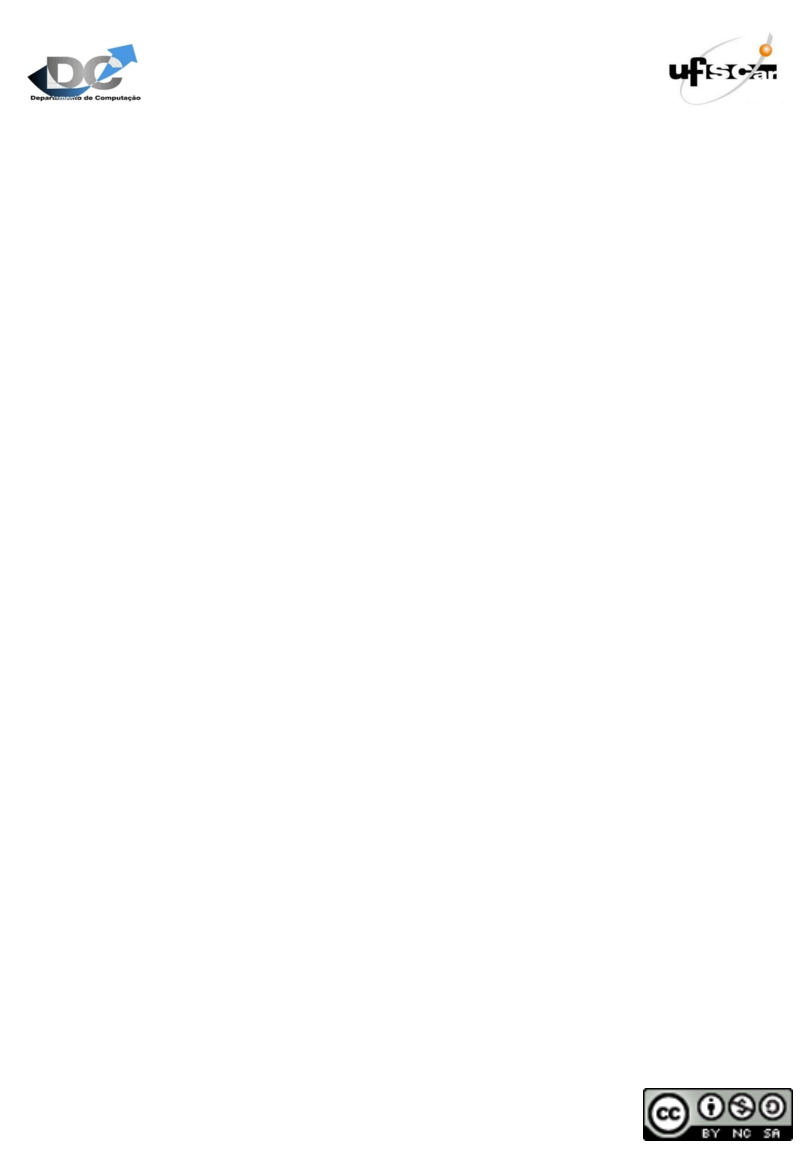
\includegraphics[scale=1]{background1}}} % Image background
\centering
\vspace*{5cm}
\par\normalfont\fontsize{32}{32}\sffamily\selectfont
\begin{figure}[h]
\centering
\includegraphics[scale=0.8]{logoGrails2}
\end{figure}
\vspace{3cm}
Desenvolvimento Web Ágil para a plataforma Java\par % Book title
\vspace*{4cm}
{\Huge 
Delano Medeiros Beder
}\par % Author name

\endgroup

%-------------------------------------------------------------------------------
%	COPYRIGHT PAGE
%-------------------------------------------------------------------------------

\newpage
~\vfill
\thispagestyle{empty}

\noindent Copyright \copyright\ 2016 Delano Medeiros Beder\\ % Copyright notice

\noindent  Esse material  está licenciado  sob a  Licença {\it  Creative Commons
  Atribuição-NãoComercial-CompartilhaIgual  3.0 Brasil}.  Para  obter uma  cópia
dessa                               licença,                              visite
\url{http://creativecommons.org/licenses/by-nc-sa/3.0/br}. 

\hspace{1cm}\\
\noindent \textit{Abril 2016} % Printing/edition date

%-------------------------------------------------------------------------------
%	TABLE OF CONTENTS
%-------------------------------------------------------------------------------

\chapterimage{chapter.pdf} % Table of contents heading image

\pagestyle{empty} % No headers

\tableofcontents % Print the table of contents itself

\cleardoublepage % Forces the first chapter to start on an odd page so it's on
                 % the right 

\pagestyle{fancy} % Print headers again

%-------------------------------------------------------------------------------
%	LISTA DE CÓDIGOS
%-------------------------------------------------------------------------------

\lstlistoflistings

%-------------------------------------------------------------------------------
%	LISTA DE FIGURAS
%-------------------------------------------------------------------------------

\listoffigures

%-------------------------------------------------------------------------------
%	LISTA DE TABELAS
%-------------------------------------------------------------------------------

\listoftables

%-------------------------------------------------------------------------------
%	CAPÍTULO 1
%-------------------------------------------------------------------------------

\pagenumbering{arabic}

\setcounter{page}{-1}

\chapterimage{chapter.pdf} % Chapter heading image

\chapter{Introdução}

É  indiscutível que  a web  se tornou  uma tecnologia  essencial  para negócios,
comércio,  educação, engenharia,  entretenimento, finanças,  governo, indústria,
mídia, medicina, política, ciência e  transporte, isso para citar apenas algumas
áreas que têm impacto sobre nossa vida.

No  entanto,  à medida  que  aplicações web  são  integradas  às estratégias  de
negócio, torna-se  cada vez mais  complexo o seu desenvolvimento.   Apesar desse
aumento de responsabilidade, o processo  de engenharia de sistemas web ainda não
é  tão  disciplinado  quanto  à  Engenharia  de  Software  tradicional.   Muitas
aplicações web  continuam a  ser construídas  de uma maneira  {\it ad  hoc}, sem
consideração com os princípios fundamentais da Engenharia de Software.

Dessa  forma, é essencial  que sistemas  passem por  um processo  de engenharia,
denominado Engenharia Web, de forma a construir e implantar uma solução eficaz e
eficiente  e que  atenda às  estratégias de  negócio e  às expectativas  de seus
usuários,  pois como  nos  demais tipos  de  software, é  necessário o  completo
entendimento  do  problema  para  se   projetar  uma  solução  eficaz  que  seja
implementada e testada corretamente.

Nesse contexto, a  Engenharia Web~\cite{Bed12, Pressman09}\index{Engenharia Web}
consiste  em  uma  abordagem  sistemática  e  ágil  para  o  desenvolvimento  de
aplicações  web. A agilidade  implica em  um enfoque  de Engenharia  de Software
enxuto que incorpora ciclos de  desenvolvimento rápidos. E cada ciclo resulta na
implantação de  um incremento da aplicação  web.  Ou seja,  o desenvolvimento da
aplicação web é realizado por meio  da entrega de uma série de versões, chamadas
de  incrementos,  que  fornecem  progressivamente mais  funcionalidade  para  os
clientes à medida que cada incremento é entregue.

Esse material  apresenta o framework web  Grails que é bem  inerente à filosofia
ágil. Na realidade, Grails, por si só não é ágil, pois nenhuma ferramenta por si
só  pode ser  ágil. No  entanto, ele  se encaixa  muito bem  com a  filosofia de
desenvolvimento ágil que sustenta que  a melhor forma de atender às necessidades
dos clientes é por meio da  colaboração de um grupo comprometido de pessoas, que
se concentra na  obtenção de resultados com rapidez, com  o mínimo de sobrecarga
possível~\cite{BA04, Schwaber04}.

O  framework Grails é  inerente a  muitas das  boas práticas  do desenvolvimento
ágil, incluindo as seguintes:

\begin{itemize}

\vspace{0.2cm}
\item  {\bf  Ser  adaptável  à   mudança}:  Graças  ao  seu  mecanismo  de  {\it
  autoreloading}   e  natureza   dinâmica,  Grails   promove  a   mudança   e  o
  desenvolvimento iterativo.

\vspace{0.2cm}
\item  {\bf Entrega  precoce do  software funcional}:  A simplicidade  de Grails
  permite uma  abordagem de desenvolvimento rápido de  aplicações, aumentando as
  probabilidades de  entrega rápida.  Além  disso, Grails prega a  automação dos
  testes   unitários   e    de   integração   (ver   Capítulo~\ref{conclusoes}),
  conscientizando os desenvolvedores de sua importância.

\vspace{0.2cm}
\item {\bf Simplicidade é  essencial}: Grails visa proporcionar simplicidade. Ou
  seja,   Grails   tem   conceitos   complexos   como   ORM   (Object-Relational
  Mapping\footnote{Mapeamento  Objeto-Relacional}),  porém  ela encapsula  esses
  conceitos em  uma API simples.  Mapeamento objeto-relacional é uma  técnica de
  desenvolvimento  de software  que é  utilizada com  o objetivo  de  reduzir os
  problemas inerentes  à utilização conjunta de  banco de dados  relacionais e o
  paradigma de desenvolvimento orientado a objetos. As tabelas do banco de dados
  são  representadas  através de  classes  e os  registros  de  cada tabela  são
  representados como instâncias das classes correspondentes.

\vspace{0.2cm}
\item {\bf Equipe entusiasmada, auto-organizada com o ambiente certo}: Desde que
  Grails  permite aos  desenvolvedores  centrar-se principalmente  na lógica  de
  negócios  necessários para  resolver um  problema  específico --  ao invés  de
  aspectos relacionados  à configuração de sua  aplicação -- a  equipe está mais
  propensa a ter desenvolvedores entusiasmados.

\end{itemize}

\section{Modelo-Visão-Controlador (MVC)}\index{Modelo-Visão-Controlador (MVC)}

\vspace{0.3cm}

Desde que o padrão arquitetural MVC é o alicerce do framework de desenvolvimento
Grails,  torna-se de fundamental  importancia apresentar  um {\it  overview} dos
principais conceitos relacionados a esse padrão arquitetural.

O modelo-visão-controlador  (MVC)~\cite{KP88, Pressman11} desacopla  a interface
com o usuário  da funcionalidade e conteúdo da  aplicação web. Uma representação
esquemática da arquitetura MVC aparece na Figura~\ref{MVCFig}. 

\begin{figure}[htbp]
\centering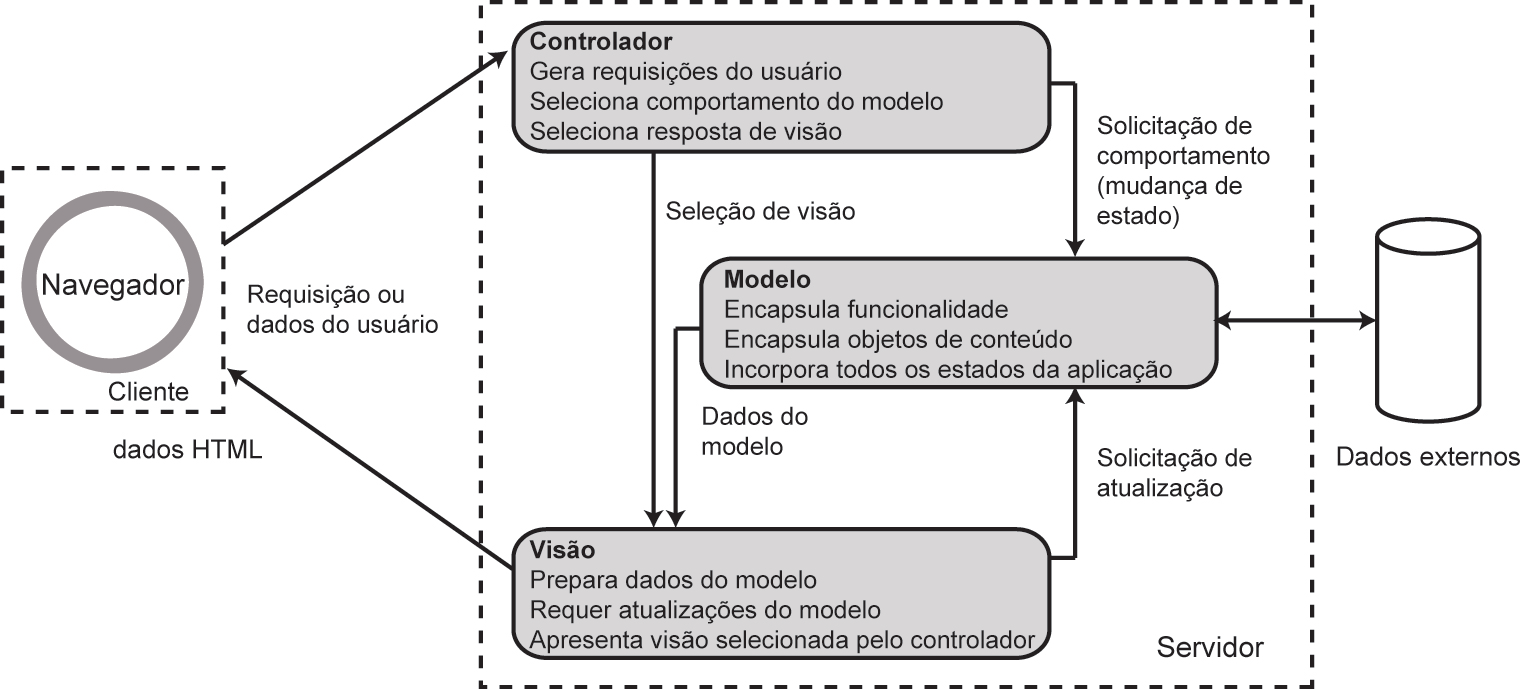
\includegraphics[width=13cm]{MVC}
\caption{Padrão arquitetural MVC}
\label{MVCFig}
\end{figure}

Esse padrão  arquitetural define três componentes (Modelo,  Visão e Controlador)
com características bem delineadas:

\begin{itemize}

\vspace{0.3cm}

\item O {\bf Modelo} contém todo  o conteúdo específico da aplicação e lógica de
  processamento, incluindo todos os objetos de conteúdo, acesso a dados externos
  e fontes  de informação, e todas  as funcionalidades de  processamento que são
  específicas da aplicação.  No caso de sistemas que utilizam  bases de dados, o
  modelo mantém  o estado persistente do  negócio e somente ele  pode acessar as
  bases de dados;

\item A {\bf Visão} contém todas as funcionalidades específicas da interface que
  habilita a apresentação de conteúdo e lógica de processamento; e

\vspace{0.3cm}

\item  O {\bf Controlador}  gerencia o  acesso e  a manipulação  do modelo  e da
  visão, bem como coordenar o fluxo de dados entre eles. Em uma aplicação web, o
  controlador monitora a interação com  o usuário e, baseando-se nisso, recupera
  os dados do modelo e utiliza-os para atualizar ou construir a visão.

\end{itemize}

\vspace{0.2cm}

\noindent  Conforme mostra a  Figura~\ref{MVCFig}, as  solicitações ou  dados do
usuário são tratados pelo controlador  que seleciona a visão apropriada com base
na  solicitação do usuário.   Quando o  tipo de  solicitação é  determinado, uma
solicitação  de  comportamento  é   transmitida  ao  modelo,  que  implementa  a
funcionalidade ou recupera  o conteúdo exigido para satisfazer  a solicitação. O
modelo pode  acessar dados  armazenados em um  banco de dados  corporativo, como
parte  de um  armazenamento  de dados  local  ou como  uma  coleção de  arquivos
independentes.   Os  dados  devolvidos   pelo  modelo  devem  ser  formatados  e
organizados pela visão apropriada e depois transmitidos do servidor da aplicação
de    volta   para   exibição    no   navegador    presente   na    máquina   do
cliente~\cite{Pressman11}. 

\section{Grails}

\vspace{0.3cm}

Grails~\cite{Grails}  é   um  framework  web  baseado   no  padrão  arquitetural
MVC~\cite{KP88} que  utiliza a  linguagem Groovy~\cite{Groovy}, executa  sobre a
máquina Virtual Java (JVM) e objetiva a alta produtividade no desenvolvimento de
aplicações      web.      Ele      combina     os      principais     frameworks
({Hibernate\footnote{\url{http://www.hibernate.org/}},
Spring\footnote{\url{http://springsource.org/}}, etc.)  utilizados na plataforma
Java e  respeita o  paradigma {\it Convention-over-configuration}  (Convenção ao
invés de Configuração).

\vspace{0.3cm}

\begin{cBox}
{\bf  Groovy.}   Groovy~\cite{Groovy} é  uma  linguagem  dinâmica,  ágil para  a
plataforma Java inspirada  em Python e Ruby que possui  sua sintaxe semelhante à
de  aplicações  desenvolvidas em  Java.   Apesar de  poder  ser  usada como  uma
linguagem  de  {\it script},  ou  seja, não  gerar  arquivos  executáveis e  não
precisar ser  compilada, Groovy  não se limita  a isso. Aplicações  feitas nesta
linguagem podem  ser compiladas utilizando-se  um compilador Java,  gerando {\it
  bytecodes}  Java (mesmo  formato da  compilação  de uma  aplicação escrita  em
Java),  além disso,  podem ser  utilizadas em  aplicações escritas  puramente em
Java.

A  linguagem foi  desenvolvida em  2004  por James  Strachan.  A  sua sintaxe  é
extremamente  parecida  com a  do  Java,  além  disso, é  possível  ``integrar''
aplicações Java e Groovy de  forma transparente. O Groovy, inclusive, simplifica
a implementação  por ``adicionar'' dinamicamente  às suas classes os  métodos de
acesso ({\bf  get} e {\bf  set}), economizando tempo  e esforço.  O  objetivo de
Groovy é simplificar a sintaxe de Java para representar comportamentos dinâmicos
como consultas  a banco de dados, escritas  e leituras de arquivos  e geração de
objetos em tempo de execução ao invés de compilação~\cite{Groovy}.

\noindent {\it  Convention Over Configuration (CoC)}.  O CoC é  um paradigma que
visa  a diminuir a  quantidade de  decisões que  o desenvolvedor  precisa tomar,
tomando como ``padrão'' algo que é  comumente usado (uma convenção). Se o padrão
escolhido pelo framework for a que o desenvolvedor precisa, este não gasta tempo
tendo que alterá-la. Entretanto, se  ele necessita de algo diferente, fica livre
para configurar  da forma que  desejar. No caso  do Grails, ele  assume diversas
configurações,  tais  como   as  de  banco  de  dados,   as  de  localização  do
código-fonte, entre outras.  \index{Convenção!{\it versus}~Configuração} 
\end{cBox}

\newpage

Este tutorial apresenta  o framework Grails apoiando o  Desenvolvimento Web Ágil
de  Software.  Uma  aplicação   denominada  {\bf  ControleBancario}  ilustra  as
diferentes etapas do processo de desenvolvimento:

\begin{itemize}

\vspace{0.3cm}

\item O capítulo~\ref{bancario} descreve  a implementação inicial das principais
  funcionalidades dessa aplicação; 

\vspace{0.3cm}

\item O capítulo~\ref{autenticacao} descreve a implementação das funcionalidades
  de autenticação de usuários no contexto dessa aplicação.  

\vspace{0.3cm}

\item  O   capítulo~\ref{autorizacao}  descreve   como  pode  ser   realizada  a
  personalização das funcionalidade presentes na aplicação ao adicionar aspectos
  relacionados à autorização do acesso às funcionalidades. 

\vspace{0.3cm}

\item   O  capítulo~\ref{interface}   descreve   como  pode   ser  realizada   a
  personalização   da   interface  da   aplicação   ao   adicionar  padrões   de
  interface.  Adicionalmente,  esse  capítulo  descreve a  implementação  de  um
  serviço {\it  web} REST  e de algumas  funcionalidades AJAX na  aplicação {\bf
    ControleBancario}.  

\vspace{0.3cm}
  
\item Finalmente, o capítulo~\ref{conclusoes} apresenta o {\it overview} de mais
  algumas  funcionalidades  presentes em  Grails  que  não  foram abordadas  nos
  capítulos anteriores.
 
\end{itemize}

\subsection{Ambiente de Desenvolvimento}
\index{Ambiente de Desenvolvimento}

\vspace{0.3cm}

Esta  seção   apresenta  alguns  pré-requisitos\footnote{Mais detalhes podem ser
  encontrados  em: \url{http://www.itexto.net/devkico/?p=40}}  do  ambiente para
apoiar o  desenvolvimento. O atendimento desses  pré-requisitos são fundamentais
para a  instalação e configuração do  ambiente de desenvolvimento  que apoiará a
compilação e execução dos exemplos discutidos neste tutorial.  A instalação do 
ambiente é simples e consiste de:

\hspace{1cm}\\
\noindent{\bf Instalação  da linguagem  Java.}  O Java  Development Kit  (JDK) –
versão  igual ou  superior a  1.5 –  será necessário  para executar  os exemplos
apresentados  nesse  material.   A última  versão  do  JDK  pode ser  obtida  em
{\footnotesize\url{http://java.com/pt_BR/download/index.jsp}}   (Esse   material
utiliza o JDK versão 1.7.0\_60). 

\vspace{0.5cm}

Dicas importantes: (1)  A variável de ambiente {\bf  JAVA\_HOME} precisa apontar
para o diretório onde o JDK foi  instalado. (2) Digite {\bf java -version} em um
terminal    para   verificar    se   o    Java   foi    instalado   corretamente
(Figura~\ref{jdkFig}).

\vspace{0.5cm}

\begin{figure}[htbp]
\centering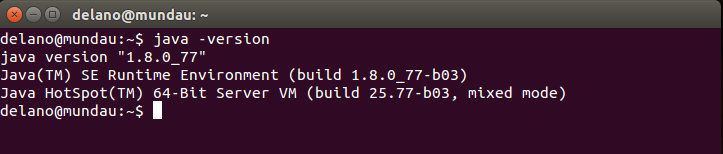
\includegraphics[width=12cm]{java}
\caption{Verificação da instalação do Java}
\label{jdkFig}
\end{figure}

\newpage

\hspace{1cm}\\ {\bf  Instalação do Grails.}   Nesse tutorial adotou-se  a versão
2.3.8       do       Grails       que       pode       ser       obtida       em
{\footnotesize\url{http://dist.springframework.org.s3.amazonaws.com/release/GRAILS/grails-2.3.8.zip}}. 
  
\hspace{1cm}\\
\noindent Após realizar o {\it download}, execute os seguintes passos:

\vspace{0.3cm}

\begin{enumerate}

  \item Descompacte  o Grails em  um diretório e  crie uma variável  de ambiente
    {\bf  GRAILS\_HOME} e  faça-o apontar  para o  diretório onde  o  Grails foi
    descompactado; e

\vspace{0.3cm}
  
  \item Adicione {\bf GRAILS\_HOME/bin} na variável de ambiente {\bf PATH}.

\end{enumerate}

\vspace{0.5cm}

\begin{figure}[htbp]
\centering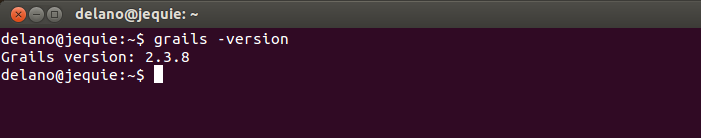
\includegraphics[width=14cm]{grails}
\caption{Verificação da instalação do Grails}
\label{grailsFig}
\end{figure}

Dica importante: Digite {\bf grails -version} em um terminal para verificar se o
Grails    foi    instalado    corretamente    e    está    pronto    para    uso
(Figura~\ref{grailsFig}). Para maiores informações sobre a instalação do Grails,
consulte                               o                               endereço:
{\footnotesize\url{http://grails.org/Installation+Portuguese}}.  

\noindent {\bf Instalação do IDE GGTS (Groovy/Grails Tool Suite).}  O IDE GGTS é
utilizado  para desenvolver  as aplicações  apresentadas nesse  tutorial.  Nesse
tutorial  foi  adotada a  versão  3.5.1  do IDE  GGTS  que  pode  ser obtida  em
{\footnotesize\url{https://spring.io/tools/ggts}} (Figura~\ref{ggtsFig}).  

\vspace{0.5cm}

\begin{figure}[htbp]
\centering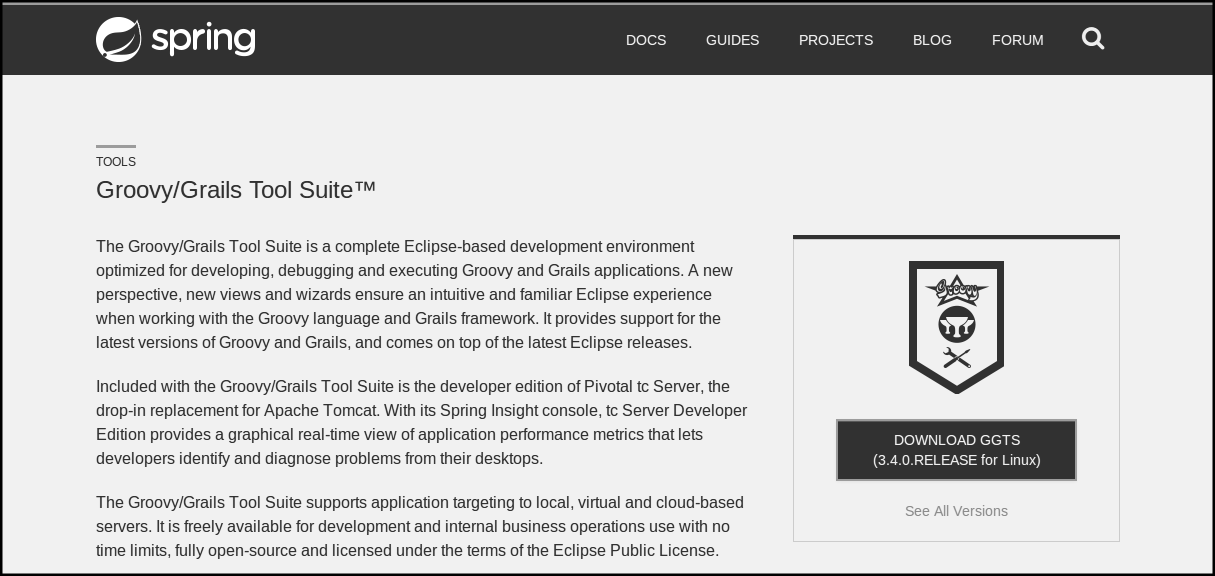
\includegraphics[width=15cm]{ggts}
\caption{Groovy/Grails Tool Suite}
\label{ggtsFig}
\end{figure}

\newpage

Ao  final da  instalação, é  necessário configurar  o IDE  GGTS  (localização do
diretório onde  foi desempacotado o Grails). Abra  o IDE GGTS, e  na janela {\bf
  Preferences}, defina a localização do Grails no Painel ``Groovy''
(Figura~\ref{ggts2Fig}). 

Embora o IDE GGTS facilite o desenvolvimento, o Grails não exige a utilização de
um IDE. Todos os comandos necessários  ao desenvolvimento podem ser feitos em um
terminal de comando. No entanto, assim como em outras linguagens de programação,
o  IDE  torna  ágil  o   processo  de  desenvolvimento  ao  integrar  diferentes
funcionalidades (edição,  compilação, execução, etc.)  e abstrair  a sintaxe dos
 comandos necessários relacionados a essas atividades. O IDE GGTS será utilizado
 neste material, mas o leitor pode usar outro IDE de seu costume.

\vspace{0.5cm}

\begin{figure}[htbp]
\centering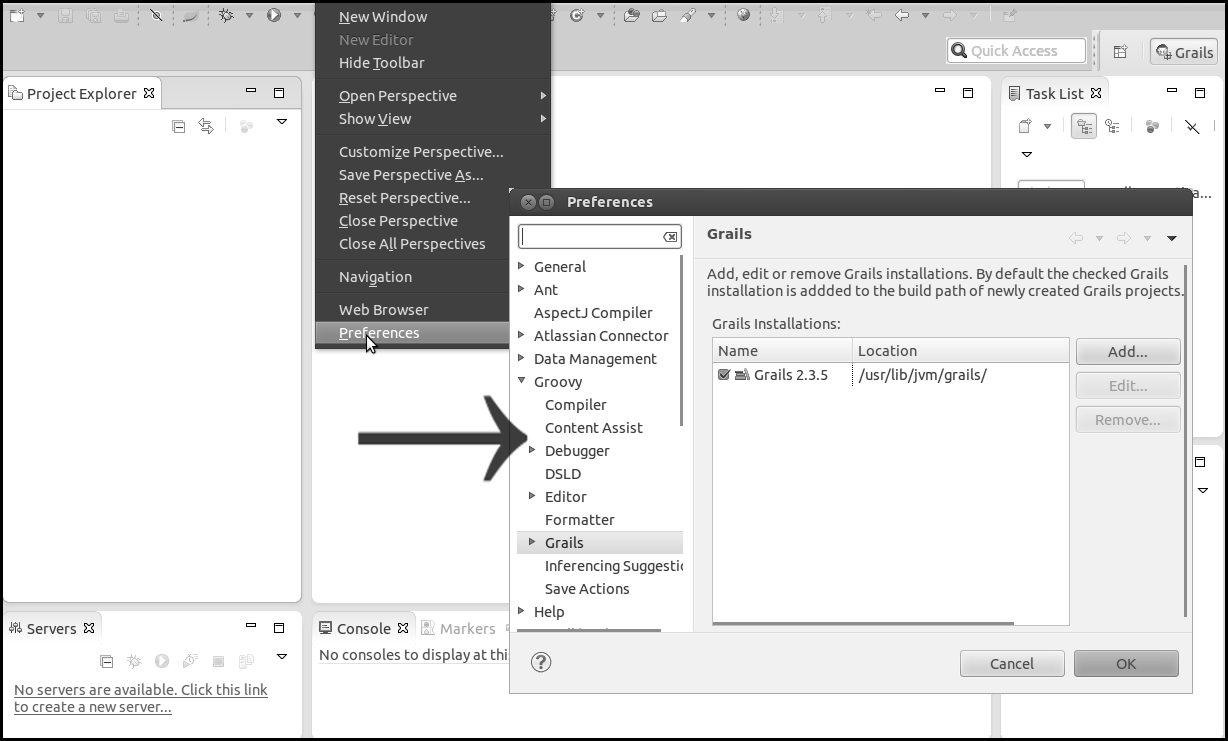
\includegraphics[width=14cm]{ggts2}
\caption{Configuração do Groovy/Grails Tool Suite}
\label{ggts2Fig}
\end{figure}
 
\vspace{0.5cm}

\noindent{\bf Banco de Dados.}\index{Banco~de~Dados}  A instalação do Grails, na
versão        adotada,       já        incorpora       uma        cópia       do
H2\footnote{\url{http://www.h2database.com/html/main.html}},   um   sistema   de
gerenciamento de banco  de dados relacional totalmente implementado  em Java que
disponibiliza um console na URI \url{/dbconsole} (Figura~\ref{H2DBFig}).  O SGBD
H2  é   útil  para  aplicações  de   demonstração,  mas  em   algum  momento  os
desenvolvedores precisarão de um SGBD mais robusto tais como MySQL, Postgresql e
Oracle. Desde que o  GORM ({\it Grails Object-Relational Mapping})\index{GORM} é
uma camada sobre o framework {\it hibernate}, qualquer banco de dados que possua
um driver JDBC e um dialeto {\it hibernate} pode ser utilizado.  

\newpage

\hspace{1cm}\\
\begin{figure}[htbp]
\centering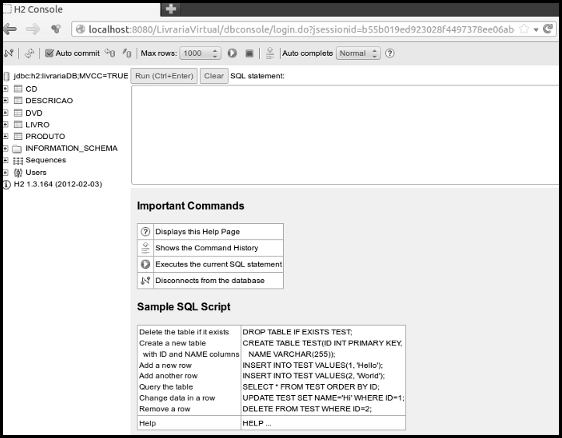
\includegraphics[height=10cm]{H2}
\caption{Console do SGBD H2}
\label{H2DBFig}
\end{figure}

\section{Considerações finais}

\vspace{0.3cm}

Esse  capítulo apresentou  um {\it  overview} das  funcionalidades  presentes em
Grails.  Dando continuidade  ao desenvolvimento  em Grails,  o  próximo capítulo
apresenta a  implementação inicial  das principais funcionalidades  da aplicação
{\bf ControleBancario}. 





%-------------------------------------------------------------------------------
%	CAPÍTULO 2
%-------------------------------------------------------------------------------

\chapter{Controle Bancário: Versão 1}\label{bancario}

Neste  capítulo, será  apresentado  o processo  de  desenvolvimento da  primeira
versão  da aplicação {\bf  ControleBancario}. Trata-se  uma aplicação  de gestão
bancária cujo modelo de entidades é apresentada na Figura~\ref{figUML}.

No IDE GGTS inicie criando um projeto, conforme apresentado a seguir:

\vspace{0.5cm}

\begin{itemize}

\item  No menu  principal,  selecione: {\bf  File}  $\Longrightarrow$ {\bf  New}
  $\Longrightarrow$ {\bf Grails Project}  (Shift-Alt-N). 

\vspace{0.5cm}

\item Em nome do projeto, digite {\bf ControleBancario} e clique em {\bf Finish}
  (Figura~\ref{criaProjFig}).   O  GGTS  IDE   executa  o  comando  {\bf  grails
  create-app}\footnote{Para obter a lista  completa de comandos Grails execute o
  comando {\bf  grails help}  em um terminal.},  apresentando a saída  na janela
  {\bf Console}.\index{Comandos!grails create-app}

\end{itemize}

\begin{figure}[htbp]
\centering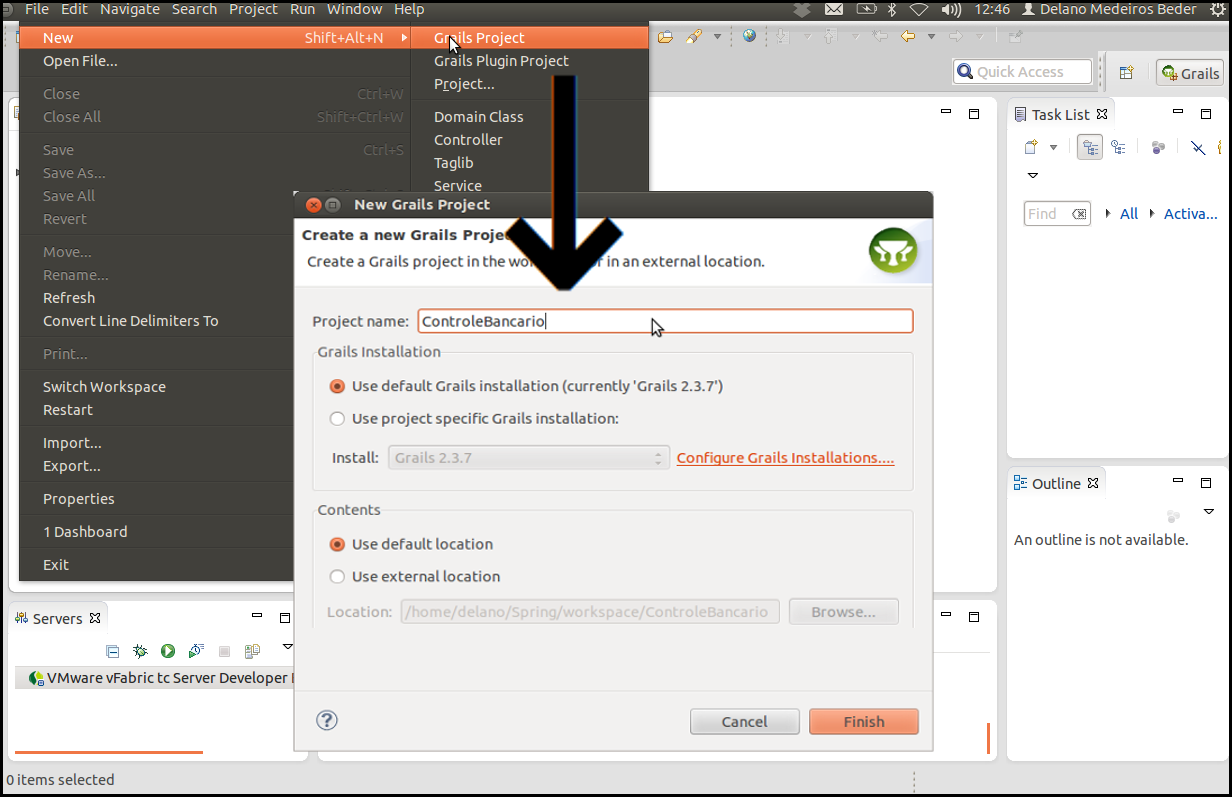
\includegraphics[width=13cm]{criaProjeto}
\caption{Criação do Projeto ControleBancario.}
\label{criaProjFig}
\end{figure}

\hspace{1cm}\\  

Caso  esses  passos  sejam  realizados  com  sucesso,  o  projeto  da  aplicação
(hierarquia  de diretórios) está  criado.  Ou  seja, foi  criado um  conjunto de
arquivos e  diretórios para  o projeto.  Essa  hierarquia de diretórios  segue o
paradigma  {\it Convention  Over  Configuration}.  Ou  seja, os  desenvolvedores
seguem  as convenções  e já  sabem {\it  a priori}  onde se  encontram  todos os
elementos  que compõem  a aplicação  em desenvolvimento.   Um {\it  overview} do
conteúdo desses diretórios é apresentado na Tabela~\ref{grailsTbl}. 
\index{Convenção!{\it versus}~Configuração}

\begin{table}[htbp]
\centering
\begin{tabular}{p{2.5cm} | p{3.5cm} | p{7.5cm}}

\toprule 
\rowcolor{Gray} 

\textbf{Aba} & \textbf{Diretório} & \textbf{Descrição}\\ 
\midrule
{\bf domain} & grails-app/domain & Onde se encontra o M do MVC. Ou seja, onde se
encontram as classes de Domínio, ou modelos.  \\ 
\midrule
{\bf controllers}  & grail-app/controllers &  Onde se encontra  o C do  MVC.  Ou
seja, onde se encontram os controladores.  \\ 
\midrule
{\bf views} & grails-app/views & Onde se  encontra o V do MVC.  Ou seja, onde se
encontram as visões (arquivos.gsp – Groovy Server Pages). \\ 
\midrule
{\bf taglibs} &  grails-app/taglib & Onde se encontram  as bibliotecas de marcas
({\it taglibs}) criadas pelo usuário. \\ 
\midrule
{\bf services} &  grails-app/services & Onde se encontram  as classes utilizadas
na camada de serviços (serviços web). \\ 
\midrule 
{\bf  i18n} & grails-app/i18n  & Onde  se encontram  os arquivos  relacionados à
internacionalização.  \\ 
\midrule
{\bf conf} & grails-app/conf &  Onde se encontram as configurações da aplicação,
tais como a  configuração do banco (DataSource.groovy), e  onde podem ser feitas
as configurações de inicialização (BootStap.groovy), entre outros. \\ 
\midrule
{\bf src/java} & src/java & Onde  se encontram outros códigos-fonte Java que não
são modelos, controladores, visões ou serviços. \\ 
\midrule   
{\bf src/groovy}  & src/groovy &  Onde se encontram outros  códigos-fonte Groovy
que não são modelos, controladores, visões ou serviços. \\ 
\midrule
{\bf  test/unit}  &  test/unit  &  Onde  se encontram  os  testes  unitários  da
aplicação.  \\ 
\midrule
{\bf  test/integration} &  test/integration &  Onde  se encontram  os testes  de
integração da aplicação.  \\ 
\midrule
{\bf lib}  & lib & Onde se  encontram as bibliotecas externas,  tais como driver
JDBC de conexão a banco de dados. \\ 
\bottomrule
\end{tabular}
\caption{Projeto Grails: {\it Overview} dos Diretórios.}
\label{grailsTbl}
\end{table}

\section{Configuração da aplicação} 

\vspace{0.5cm}

Considerando  que  o  projeto  foi  criado,  o próximo  passo  é  configurar  as
dependências   e  instalar   os  {\it   plugins}  Grails   necessários   para  o
desenvolvimento da aplicação.  

\subsection{Instalação     de      {\it     plugins}     e      definição     de
  dependências}\label{secPlugins}

\vspace{0.5cm}

Na  implementação  das  funcionalidades  da  aplicação  {\bf  ControleBancario},
discutidas nesse  capítulo, será utilizado  o plugin Grails  {\bf br-validation}
que auxilia a validação de campos CPF, CNPJ e CEP das entidades da aplicação. 

Desde  a  versão  1.3 do  Grails,  é  possível  especificar {\it  plugins}  como
dependências  -- no  arquivo  {\bf BuildConfig.groovy}  (grails-app/conf) --  ao
invés  de utilizar  o comando  {\bf grails  install-plugin}.  Dessa  forma, para
instalar     o    plugin    {\bf     br-validation}    adicione     o    comando
\texttt{compile  ":br-validation:0.3"}, descrevendo  a  dependência, no  arquivo
       {\bf   BuildConfig.groovy}   conforme   apresentado   na  linha   49   do
       Código~\ref{codBuildConfig}.  
  
\index{Comandos!grails install-plugin} 
\index{Plugins!br-validation}

\begin{lstlisting}[numbers=left, caption={\bf BuildConfig.groovy}, frame = trBL,
    float=htbp, label=codBuildConfig] 
grails.project.dependency.resolution = {
    // inherit Grails' default dependencies
    inherits("global") {
        // specify dependency exclusions here; for example, uncomment this to disable ehcache:
        // excludes 'ehcache'
    }
    log "error" // log level of Ivy resolver, either 'error', 'warn', 'info', 'debug' or 'verbose'
    checksums true // Whether to verify checksums on resolve
    legacyResolve false // whether to do a secondary resolve on plugin installation, not advised and here for backwards compatibility

    repositories {
        inherits true // Whether to inherit repository definitions from plugins

        grailsPlugins()
        grailsHome()
        mavenLocal()
        grailsCentral()
        mavenCentral()
        // uncomment these (or add new ones) to enable remote dependency resolution from public Maven repositories
        //mavenRepo "http://repository.codehaus.org"
        //mavenRepo "http://download.java.net/maven/2/"
        //mavenRepo "http://repository.jboss.com/maven2/"
    }

    dependencies {
        // specify dependencies here under either 'build', 'compile', 'runtime', 'test' or 'provided' scopes e.g.
        // runtime 'mysql:mysql-connector-java:5.1.27'
        runtime 'org.postgresql:postgresql:9.3-1100-jdbc41'
    }

    plugins {
        // plugins for the build system only
        build ":tomcat:7.0.50"

        // plugins for the compile step
        compile ":scaffolding:2.0.1"
        compile ':cache:1.1.1'

        // plugins needed at runtime but not for compilation
        runtime ":hibernate:3.6.10.7" // or ":hibernate4:4.1.11.6"
        runtime ":database-migration:1.3.8"
        runtime ":jquery:1.10.2.2"
        runtime ":resources:1.2.1"
        // Uncomment these (or add new ones) to enable additional resources capabilities
        //runtime ":zipped-resources:1.0.1"
        //runtime ":cached-resources:1.1"
        //runtime ":yui-minify-resources:0.1.5"
        
        compile ":br-validation:0.3"
    }
}
\end{lstlisting}

\newpage

\subsection{Configuração do banco de dados}\index{Banco~de~Dados}

\vspace{0.5cm}

O SGBD H2, provido pelo Grails,  é adequado para aplicações de demonstração, mas
em algum  momento os  desenvolvedores precisarão de  um SGBD mais  robusto, tais
como  {\bf  MySQL},  {\bf  Postgresql}  ou  {\bf  Oracle}.   Com  propósitos  de
ilustração, o SGBD {\bf Postgresql} será utilizado na implementação da aplicação
{\bf ControleBancario}. No entanto, o leitor pode usar outro SGBD relacional.

Para o uso de outro SGBD, tais  como {\bf MySQL} ou {\bf Oracle}, os passos para
suas  configurações são  análogos aos  apresentados a  seguir para  o  SGBD {\bf
  Postgresql}: 

\vspace{0.5cm}

\begin{itemize}

\item  Habilite  o  driver  {\it   JDBC}  do  SGBD  {\bf  Postgresql},  conforme
  apresentado na linha 28 do Código~\ref{codBuildConfig}; e 

\vspace{0.5cm}

\item Altere o arquivo {\bf grails-app/conf/DataSource.groovy} para configurar o
  acesso ({\it driver}, {\it url}, {\it  username} e {\it password}) ao banco de
  dados.  O conteúdo desse arquivo é apresentado no Código~\ref{codDataSource}.  

\end{itemize}

\vspace{0.2cm}

\begin{lstlisting}[caption={\bf  DataSource.groovy}, frame  =  trBL, float=htbp,
    label=codDataSource] 
dataSource {
    pooled = true
    driverClassName = "org.postgresql.Driver"
    username = "root"
    password = "root"
}
hibernate {
    cache.use_second_level_cache = true
    cache.use_query_cache = false
    cache.region.factory_class = 'net.sf.ehcache.hibernate.EhCacheRegionFactory' // Hibernate 3
//    cache.region.factory_class = 'org.hibernate.cache.ehcache.EhCacheRegionFactory' // Hibernate 4
}

// environment specific settings
environments {
    development {
        dataSource {
            dbCreate = "create-drop" // one of 'create', 'create-drop', 'update', 'validate', ''
            url = "jdbc:postgresql://localhost:5432/financeiro"
        }
    }
    test {
        dataSource {
            dbCreate = "update"
            url = "jdbc:postgresql://localhost:5432/financeiro"
        }
    }
    production {
        dataSource {
            dbCreate = "update"
            url = "jdbc:postgresql://localhost:5432/financeiro"
            properties {
               maxActive = -1
               minEvictableIdleTimeMillis=1800000
               timeBetweenEvictionRunsMillis=1800000
               numTestsPerEvictionRun=3
               testOnBorrow=true
               testWhileIdle=true
               testOnReturn=false
               validationQuery="SELECT 1"
               jdbcInterceptors="ConnectionState"
            }
        }
    }
}
\end{lstlisting}

\newpage

\section{Implementando as primeiras funcionalidades}\label{CRUD}

\vspace{0.5cm}

Agora que o  projeto foi criado e configurado, o próximo  passo é implementar as
primeiras funcionalidades da aplicação {\bf ControleBancario}.  É justificável iniciar pela implementação  pelas operações de CRUD das entidades
da aplicação.  CRUD é o acrônimo para  {\it Create}, {\it Read},  {\it Update} e
{\it Delete}.  Ou  seja, as operações de criação,  acesso, atualização e remoção
das  entidades  da  aplicação.   Figura~\ref{figUML} apresenta  a  modelagem  da
entidades da aplicação {\bf ControleBancario}.

\begin{figure}[h]
\centering
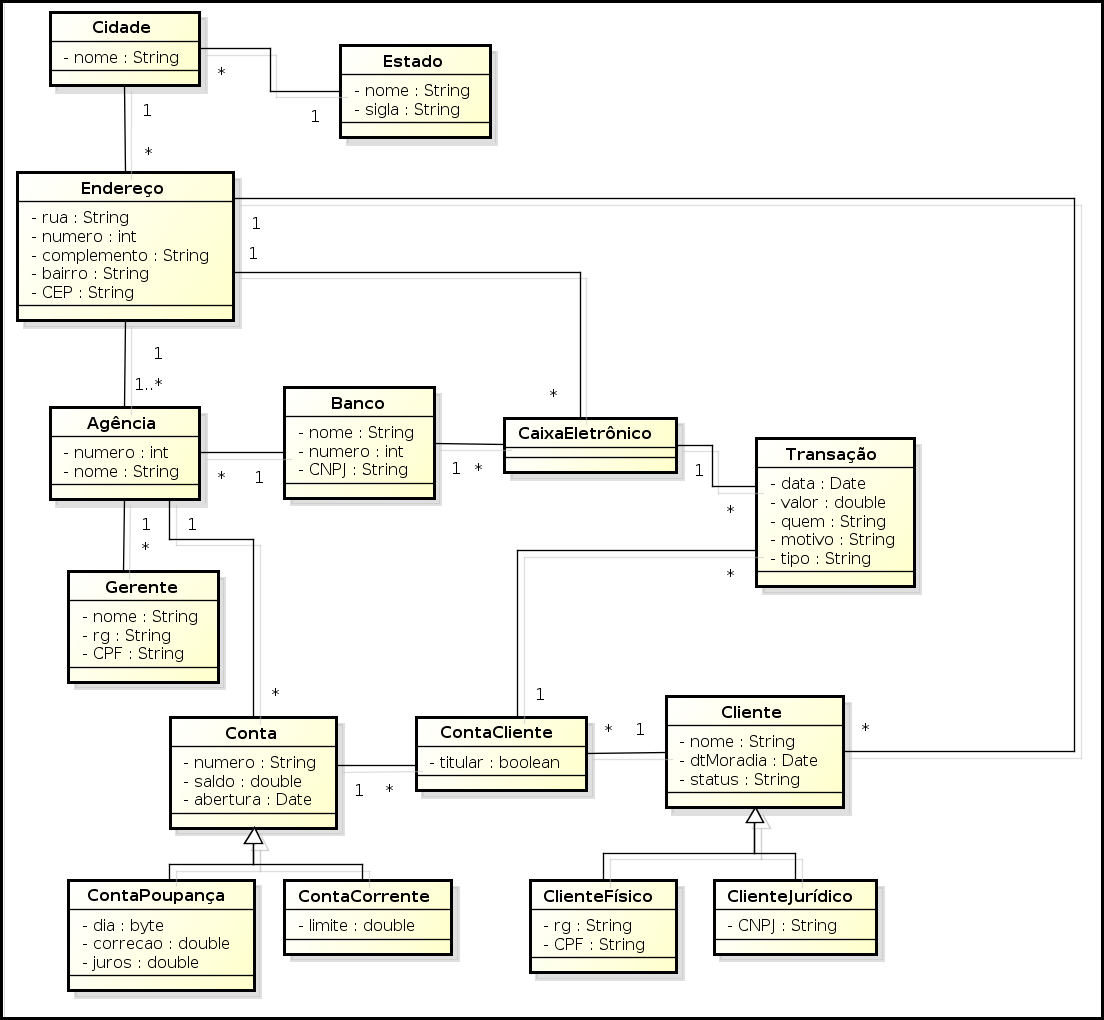
\includegraphics[width=14cm]{fig/ControleBancario}
\caption{Diagrama de classes UML}
\label{figUML}
\end{figure}

\vspace{0.5cm}

\begin{cBox}
{\bf  ControleBancario.} Essa aplicação  controla bancos,  cada um  com diversas
agências nas quais os clientes  podem realizar transações em contas correntes ou
poupanças. Um  cliente é qualquer pessoa  física ou jurídica que  abre uma conta
corrente  ou poupança  em uma  ou mais  agências de  um banco  operado  por essa
aplicação. Assim,  as  contas   estão  vinculadas  às  diferentes  agências  em
diferentes  endereços,  de  várias  cidades  em vários  estados.   Uma  conta  é
associada sempre a um cliente titular  e a zero ou mais outros clientes (segundo
titular, terceiro titular, etc). 

As transações  realizadas pelo cliente  podem ser de  retirada de valor  de suas
contas, de depósito e de transferência de valores entre contas de um mesmo banco.
\end{cBox}

Levando  em consideração o  padrão MVC~\cite{KP88},  as entidades,  presentes na
Figura~\ref{figUML}, fazem parte do modelo (o  M do MVC) da aplicação.  Assim, é
necessário  criar  uma classe  de  Domínio\footnote{Em  Grails,  os modelos  são
  denominados  de classes  de domínio.}   para cada  entidade da  aplicação {\bf
  ControleBancario}\index{Modelo-Visão-Controlador (MVC)!Modelo}.  

\subsection{Classe de Domínio: Estado}\label{secEstado}

\vspace{0.5cm}

A primeira  classe de  domínio a ser  implementada é  a classe {\bf  Estado} que
representa os estados brasileiros.

\begin{itemize}

\item  Para criá-la  no IDE  GGTS,  selecione {\bf  New} $\Longrightarrow$  {\bf
  Domain Class} (Figura~\ref{novoEstadoFig}).

\vspace{0.5cm}

\item Digite  {\bf br.ufscar.dc.dsw.Estado} como o  nome da classe  de domínio e
  clique  em  {\bf   Finish}.   O  GGTS  IDE  executa   o  comando  {\bf  grails
    create-domain-class}, apresentando a saída na janela {\bf Console}. A classe
  de    domínio   {\bf    Estado.groovy}    é   criada    no   diretório    {\bf
    grails-app/domain}. \index{Comandos!grails create-domain-class} 

\vspace{0.5cm}

\item  Abra a  classe {\bf  Estado} e  insira os  atributos ({\bf  nome}  e {\bf
  sigla}) dessa classe conforme apresentado no Código~\ref{codEstado}. 

\end{itemize}

\begin{figure}[htbp]
\centering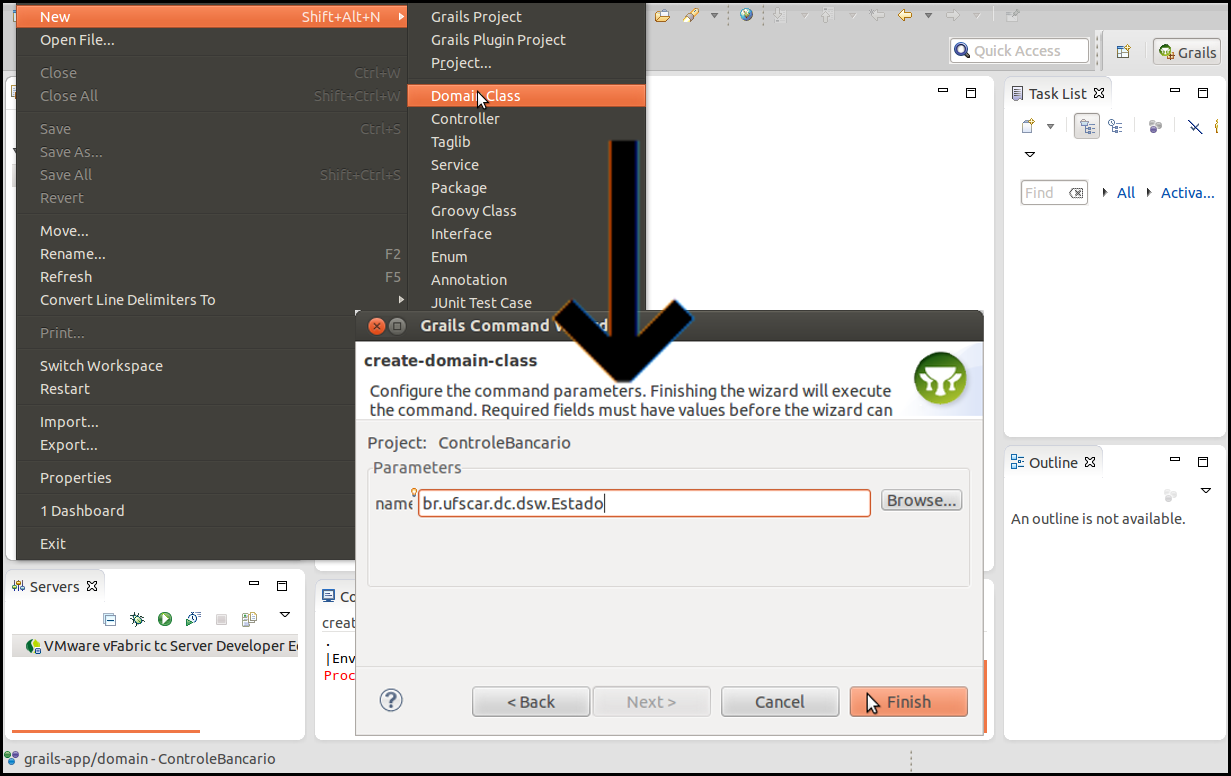
\includegraphics[width=12cm]{novoEstado}
\caption{Criação da Classe de Domínio Estado.}
\label{novoEstadoFig}
\end{figure}

\hspace{1cm}\\
\noindent {\bf Observações:}

\begin{itemize}

\item O  atributo {\bf  id} é  gerado automaticamente pelo  Grails. Logo,  não é
  necessário incluí-lo na implementação da classe {\bf Estado}; 

\vspace{0.2cm}

\item A classe de domínio {\bf Estado} possui os seguintes atributos:

\vspace{0.2cm}

\begin{itemize}

\item[$\diamond$] {\bf nome} -- que armazena o nome do estado;

\vspace{0.2cm}

\item[$\diamond$] {\bf  sigla} -- que armazena  a sigla do  estado (por exemplo:
  {\bf SP} para o estado de São Paulo); 

\end{itemize}

\vspace{0.5cm}

\item O método {\bf toString()} retorna  uma representação (por exemplo, o que é
  apresentada nas visões – páginas HTML) das instâncias das classes.  No caso da
  implementação da  classe de  domínio {\bf Estado},  o método  {\bf toString()}
  retorna a sigla do estado.
 
\end{itemize}

\newpage

\begin{lstlisting}[caption=Classe  de  domínio   {\bf  Estado},  frame  =  trBL,
    float=htbp, label=codEstado] 
package br.ufscar.dc.dsw

class Estado {

    static constraints = {
        nome (nullable: false, size: 1..20)
        sigla (nullable: false, size: 2..2)
    }
    
    String nome    
    String sigla
    
    String toString() {
        return sigla
    }
}
\end{lstlisting}

\subsubsection{Validação de Dados}\index{Validação de Dados}\label{validacao}

\vspace{0.5cm}

\noindent  O  bloco {\bf  static  constraints}  permite  que os  desenvolvedores
coloquem regras  de validação nas classes  de domínio.  Por  exemplo, é possível
impor restrições  sobre o tamanho  máximo de um  atributo String (por  padrão, o
tamanho é 255 caracteres).  Além disso,  é possível garantir que campos de texto
(Strings) correspondem  a um determinado padrão  (como um endereço  de e-mail ou
URL). E por fim, é possível até mesmo tornar campos opcionais ou obrigatórios.

Além  dessas validações,  o bloco  {\bf static  constraints}  também possibilita
definir a  ordem em que  os atributos de  um modelo são apresentados  nas visões
associadas.   O Código  ~\ref{codEstado} descreve  o  uso do  bloco {\bf  static
  constraints}  para validar os  atributos da  classe {\bf  Estado} e  definir a
ordem   em    que   os   atributos    dessa   classe   são    apresentados.    A
Tabela~\ref{restricoesTbl}   apresenta  algumas   restrições  com   exemplos  de
utilização e respectivas descrições.

\begin{table}[htbp]
\centering
\begin{footnotesize}
\begin{tabular}{p{2.0cm} | p{4.5cm} | p{6.5cm}}
\toprule     
\rowcolor{Gray}     
\textbf{Nome}     &     \textbf{Exemplo}     & \textbf{Descrição}\\  
\midrule 
blank &  nome(blank:false) & Coloque {\bf false}  se o valor da  String não pode
estar em branco.\\
\midrule
email &  e-mail(email:true) & Coloque {\bf  true} se a String  necessitar ser um
endereço de e-mail válido.\\
\midrule 
inList & sexo(inList:["F", "M"]) & O valor deve estar contido
na  lista.  \\  
\midrule  
length &  nome(length:5..15) & Usa  uma faixa para  restringir o tamanho  de uma
String ou array.\\
\midrule
min & quantidade(min:0) & Define o valor mínimo. \\
\midrule 
matches  & nome(matches:/[a-zA-Z]/) &  Verifica se  corresponde a  uma expressão
regular fornecida.  \\
\midrule   
max & quantidade(max:100) & Define o valor máximo. \\
\midrule
nullable &  preco(nullable:false) & Coloque {\bf  false} se o  valor do atributo
não poder ser nulo. \\
\midrule  
range  &  quantidade(range:5..15)  &   Valor  deve  estar  dentro  do  intervalo
especificado.  \\
\midrule  
size  & list(size:5..15)  &  Usa uma  faixa  para restringir  o  tamanho de  uma
coleção.\\
\midrule  
unique & nome(unique:true)  & Defina como {\bf true} se o  valor do atributo não
pode repetir. \\
\midrule
url & homepage(url:true)  & Defina como {\bf true} se o valor da String precisar
ser um endereço URL válido.  \\
\bottomrule
\end{tabular}
\end{footnotesize}
\caption{Regras de restrições.}
\label{restricoesTbl}
\end{table}

\newpage

\subsection{Classe de Domínio: Cidade}\label{secCidade}

\vspace{0.5cm}

A próxima classe de domínio a ser  criada é a classe {\bf Cidade} que representa
cidades brasileiras.  

Crie,  usando os  mesmos passos  da criação  da classe  de domínio  {\bf Estado}
(Seção~\ref{secEstado}), a classe {\bf Cidade} do pacote {\bf br.ufscar.dc.dsw}.
Abra a classe {\bf Cidade}, insira os atributos e acrescente as suas validações,
conforme apresentado no Código~\ref{codCidade}.  

\begin{lstlisting}[caption=Classe  de  domínio   {\bf  Cidade},  frame  =  trBL,
    float=htbp, label=codCidade] 
package br.ufscar.dc.dsw

class Cidade {

    static constraints = {
        nome (blank: false, size: 1..40)
        estado (nullable: false)
    }

    String nome
    Estado estado
    
    String toString() {
        StringBuilder sb = new StringBuilder();
        if (nome != null) {
            sb.append(nome)
            sb.append(" - ")
            sb.append(estado.sigla)
        }
        return sb.toString();
    }
}
\end{lstlisting}

\hspace{1cm}\\
\noindent {\bf Observações:}
\hspace{1cm}\\

\begin{itemize}

\item A classe de domínio {\bf Cidade} possui os seguintes atributos:

\vspace{0.2cm}

\begin{itemize}

\item[$\diamond$] {\bf nome} -- que armazena o nome da cidade;

\vspace{0.2cm}

\item[$\diamond$] {\bf estado} -- que armazena uma referência a uma instância da
  classe {\bf Estado}.   Esse atributo é um mapeamento  unidirecional entre {\bf
    Cidade} e {\bf  Estado}.  Pelos requisitos da aplicação,  não há necessidade
  de implementar um mapeamento bidirecional entre essas duas classes de domínio.

\end{itemize}

\end{itemize}

\vspace{0.5cm}

\begin{cBox}
Uma  importante característica  do Grails  é que  programadores não  precisam se
preocupar em criar  os métodos {\it getters} e {\it  setters}.  Eles são gerados
pelo Groovy.  Grails, por meio  do mecanismo GORM ({\it Grails Object-Relational
  Mapping})\index{GORM}, realiza um mapeamento automático entre modelos (classes
de domínio) e tabelas em um SGBD.

Dessa forma, o Groovy gera outros métodos estáticos responsáveis pelas operações
{\it CRUD} ({\it Create}, {\it Read}, {\it Update} e {\it Delete}): 

\begin{itemize}

\item {\bf Cidade.save()} armazena os dados na tabela Cidade (do SGBD).

\item {\bf Cidade.delete()} apaga os dados da tabela Cidade.

\item {\bf Cidade.list()} retorna uma lista de cidades.

\item {\bf Cidade.get()} retorna uma única instância da classe Cidade.

\end{itemize}

Todos esses  e outros métodos  estão disponíveis para os  desenvolvedores.  Note
que  {\bf  Cidade}  não  estende  nenhuma  classe  pai  nem  implementa  nenhuma
interface.   Graças  aos  recursos  de  metaprogramação  Groovy,  esses  métodos
simplesmente  aparecem  quando  necessários.   Apenas as  classes  presentes  no
diretório {\bf  grails-app/domain} (ou seja,  classes de domínio)  possuem esses
métodos relacionados à persistência de dados: {\bf save()}, {\bf delete()}, {\bf
  list()} e {\bf get()}.
\end{cBox}

\newpage

\subsection{Classe de Domínio: Endereco}\label{secEndereco}

\vspace{0.5cm}

Crie,  usando os  mesmos passos  da criação  da classe  de domínio  {\bf Estado}
(Seção~\ref{secEstado}),    a   classe   {\bf    Endereco}   do    pacote   {\bf
  br.ufscar.dc.dsw}.   Abra  a classe  {\bf  Endereco},  insira  os atributos  e
acrescente     as      suas     validações,     conforme      apresentado     no
Código~\ref{codEndereco}. 

\begin{lstlisting}[caption=Classe  de  domínio  {\bf  Endereco}, frame  =  trBL,
    float=htbp, label=codEndereco]
package br.ufscar.dc.dsw

class Endereco {

    static constraints = {
        CEP (blank: false, cep: true, size: 9..9)
        logradouro (blank: false, size: 1..40)
        numero (min: 0)
        complemento (nullable: true, size: 1..40)
        bairro (blank: false, size: 1..40)
        cidade (nullable: false)
    }
    
    String logradouro
    
    int numero
    
    String complemento
    
    String bairro
    
    String CEP
    
    Cidade cidade
    
    String toString() {
        return logradouro + ", " + numero + 
               (complemento == null ? "" : " " + complemento) + ". " + 
               bairro + " " + CEP + " " + cidade 
    }
} 
\end{lstlisting}

\hspace{1cm}\\
\noindent {\bf Observações:}
\hspace{1cm}\\

\begin{itemize}

\item A classe de domínio {\bf Endereco} possui os seguintes atributos:

\vspace{0.5cm}

\begin{itemize}

\item[$\diamond$] {\bf logradouro} -- que armazena o nome do logradouro;

\vspace{0.5cm}

\item[$\diamond$] {\bf numero} -- que armazena o número do endereço;

\vspace{0.5cm}

\item[$\diamond$] {\bf complemento} -- que armazena o complemento de endereço;

\vspace{0.5cm}

\item[$\diamond$] {\bf bairro} -- que armazena o bairro do endereço;

\vspace{0.5cm}

\item[$\diamond$] {\bf CEP} -- que armazena o CEP de endereço. A validação desse
  atributo utiliza a  restrição {\bf cep: true} definida  pelo {\it plugin} {\bf
    br-validation} instalado na Seção~\ref{secPlugins}; e

\vspace{0.5cm}

\item[$\diamond$] {\bf cidade} -- que armazena uma referência a uma instância da
  classe  {\bf Cidade}  (Seção~\ref{secCidade}). Esse  atributo é  um mapeamento
  unidirecional  entre  {\bf Endereco}  e  {\bf  Cidade}.   Pelos requisitos  da
  aplicação, não há necessidade  de implementar um mapeamento bidirecional entre
  essas duas classes de domínio.  

\end{itemize}

\vspace{0.5cm}

\item O  método {\bf  toString()} retorna uma  representação das  instâncias das
  classes.   No caso da  implementação da  classe de  domínio {\bf  Endereco}, o
  método  {\bf  toString()} retorna  uma  descrição  textual  do endereço  (rua,
  número, complemento, bairro, CEP e cidade).

\end{itemize}

\newpage

\subsection{Classe de Domínio: Banco}\label{secBanco}

\vspace{0.5cm}

A próxima classe de  domínio a ser criada é a classe  {\bf Banco} que representa
instituições bancárias.  Crie,  usando os mesmos passos da  criação da classe de
domínio  {\bf Estado} (Seção~\ref{secEstado}),  a classe  {\bf Banco}  do pacote
{\bf  br.ufscar.dc.dsw}.  Abra  a  classe  {\bf Banco},  insira  os atributos  e
acrescente as suas validações, conforme apresentado no Código~\ref{codBanco}. 

\begin{lstlisting}[caption=Classe  de   domínio  {\bf  Banco},   frame  =  trBL,
    float=htbp, label=codBanco] 
package br.ufscar.dc.dsw

class Banco {

    static hasMany = [agencias: Agencia, caixas: CaixaEletronico]

    static constraints = {
        numero (unique: true, min: 0)
        nome (blank: false, size: 1..20)
        CNPJ (blank: false, unique:true, cnpj: true, size: 18..18)
    }

    int numero
    String nome
    String CNPJ

    String toString() {
        return nome
    }
}
\end{lstlisting}

\hspace{1cm}\\
\noindent {\bf Observações:}
\hspace{1cm}\\

\begin{itemize}

\item A classe de domínio {\bf Banco} possui os seguintes atributos:

\vspace{0.5cm}

\begin{itemize}

\item[$\diamond$] {\bf numero}  -- que armazena o número  (único) da instituição
  bancária; 

\vspace{0.5cm}

\item[$\diamond$] {\bf nome} -- que armazena o nome da instituição bancária; e

\vspace{0.5cm}

\item[$\diamond$] {\bf CNPJ} -- que  armazena o CNPJ da instituição bancária.  A
  validação desse  atributo utiliza a  restrição {\bf cnpj: true}  definida pelo
  {\it plugin} {\bf br-validation} instalado na Seção~\ref{secPlugins}.

\end{itemize}

\vspace{0.5cm}

\item O comando {\bf static hasMany  = [agencias: Agencia]} na classe de domínio
  {\bf  Banco} e  o atributo  {\bf  banco} na  classe de  domínio {\bf  Agencia}
  (Seção~\ref{secAgencia}),  foram utilizados  em conjunto  para  implementar um
  mapeamento {\em um-para-muitos} entre essas classes.
 
\vspace{0.5cm}

\item O  comando {\bf static hasMany  = [caixas: CaixaEletronico]}  na classe de
  domínio  {\bf Banco}  e  o atributo  {\bf  banco} na  classe  de domínio  {\bf
    CaixaEletronico}   (Seção~\ref{secCaixaEletronico}),  foram   utilizados  em
  conjunto  para  implementar um  mapeamento  {\em  um-para-muitos} entre  essas
  classes.

\vspace{0.5cm}

\item O  método {\bf  toString()} retorna uma  representação das  instâncias das
  classes.  No caso da implementação da  classe de domínio {\bf Banco}, o método
  {\bf toString()} retorna apenas o nome do banco.

\end{itemize}

\newpage

\subsection{Classe de Domínio: Agencia}\label{secAgencia}

\vspace{0.5cm}

A  classe   de  domínio  {\bf  Agencia}  representa   agências  de  instituições
bancárias. Crie a classe {\bf Agencia} do pacote {\bf br.ufscar.dc.dsw}.  Abra a
classe  {\bf Agencia},  insira os  atributos  e acrescente  as suas  validações,
conforme apresentado no Código~\ref{codCidade}. 

\begin{lstlisting}[caption=Classe  de  domínio  {\bf  Agencia},  frame  =  trBL,
    float=htbp, label=codAgencia] 
package br.ufscar.dc.dsw

class Agencia {

    static hasMany = [gerentes: Gerente]

    static constraints = {
        banco (nullable: false)
        numero (blank: false, min: 0)
        nome (blank: false, size: 1..20)
        endereco (nullable: false)
    }

    int numero
    String nome
    Endereco endereco
    Banco banco

    String toString() {
        StringBuilder sb = new StringBuilder();
        sb.append(numero)
        sb.append(" - ")
        sb.append(banco)
        return sb.toString();
    }
}
\end{lstlisting}

\hspace{1cm}\\
\noindent {\bf Observações:}
\hspace{1cm}\\

\begin{itemize}

\item A classe de domínio {\bf Agencia} possui os seguintes atributos:

\vspace{0.5cm}

\begin{itemize}

\item[$\diamond$] {\bf numero} -- que armazena o número da agência bancária; 

\vspace{0.5cm}

\item[$\diamond$] {\bf nome} -- que armazena o nome da agência bancária; 

\vspace{0.5cm}

\item[$\diamond$] {\bf endereco} -- que  armazena uma referência a uma instância
  da classe de domínio  {\bf Endereco} (Seção~\ref{secEndereco}).  Esse atributo
  é um  mapeamento unidirecional  entre {\bf Agencia}  e {\bf  Endereco}.  Pelos
  requisitos  da aplicação,  não  há necessidade  de  implementar um  mapeamento
  bidirecional entre essas duas classes de domínio; e

\vspace{0.5cm}

\item[$\diamond$] {\bf banco} -- que  armazena uma referência a uma instância da
  classe   de  domínio  {\bf   Banco}  (Seção~\ref{secBanco}).    Esse  atributo
  representa a cardinalidade {\em ``um''} do relacionamento {\em um-para-muitos}
  entre as classes de domínio {\bf Banco} e {\bf Agencia}.

\end{itemize}

\vspace{0.5cm}

\item O comando {\bf static hasMany  = [gerentes: Gerente]} na classe de domínio
  {\bf Agencia}  e o atributo {\bf  agencia} na classe de  domínio {\bf Gerente}
  (Seção~\ref{secGerente}),  foram  utilizados em  conjunto  para implementar  o
  mapeamento  {\em  um-para-muitos}  entre  as  classes  {\bf  Agencia}  e  {\bf
    Gerente}.

\vspace{0.5cm}

\item O  método {\bf  toString()} retorna uma  representação das  instâncias das
  classes.   No caso  da implementação  da classe  de domínio  {\bf  Agencia}, o
  método {\bf toString()} retorna o número  da agência concatenado com o nome do
  banco.

\end{itemize}

\newpage

\subsection{Classe de Domínio: Gerente}\label{secGerente}

\vspace{0.5cm}

A  classe  de   domínio  {\bf  Gerente}  representa  gerentes   de  agências  de
instituições   bancárias.  Crie   a  classe   {\bf  Gerente}   do   pacote  {\bf
  br.ufscar.dc.dsw}.   Abra  a  classe  {\bf  Gerente}, insira  os  atributos  e
acrescente as suas validações, conforme apresentado no Código~\ref{codGerente}.  

\begin{lstlisting}[caption=Classe  de  domínio  {\bf  Gerente},  frame  =  trBL,
    float=htbp, label=codGerente] 
package br.ufscar.dc.dsw

class Gerente {

    static constraints = {
        nome (blank: false, size: 1..30)
        rg (blank: false, size: 1..12)
        CPF (blank: false, unique: true, cpf: true, size: 14..14)
        agencia (nullable: false)
    }

    String nome
    String rg
    String CPF
    Agencia agencia
    
    String toString() {
        return nome + " " + CPF
    }
}
\end{lstlisting}

\hspace{1cm}\\
\noindent {\bf Observações:}
\hspace{1cm}\\

\begin{itemize}

\item A classe de domínio {\bf Gerente} possui os seguintes atributos:

\vspace{0.5cm}

\begin{itemize}

\item[$\diamond$] {\bf nome} -- que armazena o nome do gerente; 

\vspace{0.5cm}

\item[$\diamond$] {\bf rg} -- que armazena o RG do gerente; 

\vspace{0.5cm}

\item[$\diamond$] {\bf CPF} -- que  armazena o CPF do gerente.  A
  validação desse  atributo utiliza a  restrição {\bf cpf: true}  definida pelo
  {\it plugin} {\bf br-validation} instalado na Seção~\ref{secPlugins}; e

\vspace{0.5cm}

\item[$\diamond$] {\bf agencia}  -- que armazena uma referência  a uma instância
  da classe  de domínio  {\bf Agencia} (Seção~\ref{secAgencia}).   Esse atributo
  representa a cardinalidade {\em ``um''} do relacionamento {\em um-para-muitos}
  entre as classes de domínio {\bf Agencia} e {\bf Gerente}.

\end{itemize}

\vspace{0.5cm}

\item O  método {\bf  toString()} retorna uma  representação das  instâncias das
  classes.   No caso  da implementação  da classe  de domínio  {\bf  Gerente}, o
  método  {\bf  toString()}  retorna  o  nome do  gerente  concatenado  com  seu
  respectivo CPF.

\end{itemize}

\newpage

\subsection{Classe de Domínio: CaixaEletronico}\label{secCaixaEletronico}

\vspace{0.5cm}

A  classe  de  domínio  {\bf  CaixaEletronico}  representa  caixas  eletrônicos,
pertencentes    às   instituições    bancárias,   onde    transações   bancárias
(Seção~\ref{secTransacao})   podem   ser  realizadas.    Crie   a  classe   {\bf
  CaixaEletronico}  do  pacote  {\bf  br.ufscar.dc.dsw}.   Abra  a  classe  {\bf
  CaixaEletronico},  insira  os  atributos  e  acrescente  as  suas  validações,
conforme apresentado no Código~\ref{codCaixaEletronico}. 

\begin{lstlisting}[caption=Classe  de  domínio  {\bf CaixaEletronico},  frame  =
    trBL, float=htbp, label=codCaixaEletronico] 
package br.ufscar.dc.dsw

class CaixaEletronico {

    static hasMany = [transacoes: Transacao]
    
    static constraints = {
        banco (nullable: false)
        endereco (nullable: false)
    }
    
    Endereco endereco
    Banco banco
    
    String toString() {
        return banco.toString() + " - " + endereco.toString();
    }
}
\end{lstlisting}

\hspace{1cm}\\
\noindent {\bf Observações:}
\hspace{1cm}\\

\begin{itemize}

\item A classe de domínio {\bf CaixaEletronico} possui os seguintes atributos: 

\vspace{0.5cm}

\begin{itemize}

\item[$\diamond$] {\bf banco} -- que  armazena uma referência a uma instância da
  classe de domínio {\bf  Banco} (Seção~\ref{secBanco}).  Ou seja, esse atributo
  representa a cardinalidade {\em ``um''} do relacionamento {\em um-para-muitos}
  entre as classes de domínio {\bf Banco} e {\bf CaixaEletronico}; e

\vspace{0.5cm}

\item[$\diamond$] {\bf endereco} -- que  armazena uma referência a uma instância
  da classe de domínio  {\bf Endereco} (Seção~\ref{secEndereco}).  Esse atributo
  é um  mapeamento unidirecional entre  {\bf CaixaEletronico} e  {\bf Endereco}.
  Pelos requisitos da aplicação, não há necessidade de implementar um mapeamento
  bidirecional entre essas duas classes de domínio.

\end{itemize}

\vspace{0.5cm}

\item  O comando {\bf  static hasMany  = [transacoes:  Transacao]} na  classe de
  domínio {\bf CaixaEletronico} e o  atributo {\bf caixaEletronico} na classe de
  domínio  {\bf  Transacao}   (Seção~\ref{secTransacao}),  foram  utilizados  em
  conjunto  para  implementar  o  mapeamento {\em  um-para-muitos}  entre  essas
  classes de domínio.

\vspace{0.5cm}

\item O  método {\bf  toString()} retorna uma  representação das  instâncias das
  classes.  No caso da implementação da classe de domínio {\bf CaixaEletronico},
  o método {\bf  toString()} retorna o nome do banco  concatenado com o endereço
  do caixa eletrônico.

\end{itemize}

\newpage

\subsection{Classe de Domínio: Transacao}\label{secTransacao}

\vspace{0.5cm}

A classe de  domínio {\bf Transacao} representa transações  realizadas em contas
bancárias vinculadas a clientes do  banco.  Pelos requisitos da aplicação, todas
as transações bancárias são realizadas em um caixa eletrônico.

Crie a classe  {\bf Transacao} do pacote {\bf  br.ufscar.dc.dsw}.  Abra a classe
{\bf Transacao}, insira  os atributos e acrescente as  suas validações, conforme
apresentado no Código~\ref{codTransacao}.  

\begin{lstlisting}[caption=Classe  de  domínio {\bf  Transacao},  frame =  trBL,
    float=htbp, label=codTransacao] 
package br.ufscar.dc.dsw

class Transacao {
    
    public static final String CR^É^DITO = "CR^É^DITO"
    public static final String D^É^BITO = "D^É^BITO"
    
    static constraints = {
        contaCliente (nullable: false)
        caixaEletronico (nullable: false)
        valor (nullable: false, min: 0.1d)
        data (nullable: false)
        quem (nullable: false)
        motivo (nullable: false)
        tipo (nullable: false, inList: [CR^É^DITO,D^É^BITO])
    }
        
    Date data
    
    double valor
    
    String quem
    
    String motivo
    
    String tipo
    
    ContaCliente contaCliente
    
    CaixaEletronico caixaEletronico

    String toString() {
        return "[" + tipo + "] - " + motivo + " - R\$ " + valor 
    }
}
\end{lstlisting}

\noindent {\bf Observações:}
\hspace{1cm}\\

\begin{itemize}

\item A classe de domínio {\bf Transacao} possui os seguintes atributos:

\vspace{0.3cm}

\begin{itemize}

\item[$\diamond$] {\bf data} -- que armazena a data em que ocorreu a transação; 

\vspace{0.3cm}

\item[$\diamond$] {\bf valor} -- que armazena o valor da transação; 

\vspace{0.3cm}

\item[$\diamond$] {\bf quem} -- que armazena {\em quem} realizou a transação; 

\vspace{0.3cm}

\item[$\diamond$] {\bf motivo} -- que  armazena {\em o motivo} (saque, depósito,
  transferência) da transação;

\vspace{0.3cm}

\item[$\diamond$] {\bf tipo} -- que  armazena o tipo de transação: {\bf Crédito}
  ou {\bf Débito};

\vspace{0.3cm}

\item[$\diamond$]  {\bf  contaCliente} --  que  armazena  uma  referência a  uma
  instância      da      classe      de     domínio      {\bf      ContaCliente}
  (Seção~\ref{secContaCliente}).  Esse atributo  representa a cardinalidade {\em
    ``um''} do  relacionamento {\em um-para-muitos} entre as  classes de domínio
  {\bf ContaCliente} e {\bf Transacao}.

\vspace{0.3cm}

\item[$\diamond$]  {\bf caixaEletronico} --  que armazena  uma referência  a uma
  instância     da      classe     de     domínio      {\bf     CaixaEletronico}
  (Seção~\ref{secCaixaEletronico}).   Ou   seja,  esse  atributo   representa  a
  cardinalidade  {\em ``um''}  do relacionamento  {\em um-para-muitos}  entre as
  classes de domínio {\bf CaixaEletronico} e {\bf Transacao}.

\end{itemize}

\end{itemize}

\newpage

\subsection{Classe de Domínio: ContaCliente}\label{secContaCliente}

\vspace{0.5cm}

A  classe  de  domínio  {\bf  ContaCliente} materializa  o  relacionamento  {\em
  muitos-para-muitos} entre as classes de domínio {\bf Conta} e {\bf Cliente}. O
relacionamento  {\em muitos-para-muitos}  entre {\bf  Conta} e  {\bf  Cliente} é
obtido ao implementar dois relacionamentos {\em um-para-muitos}: (i) {\bf Conta}
x {\bf ContaCliente} e (ii) {\bf Cliente} x {\bf ContaCliente}.

Crie  a classe  {\bf ContaCliente}  do  pacote {\bf  br.ufscar.dc.dsw}.  Abra  a
classe {\bf ContaCliente}, insira os  atributos e acrescente as suas validações,
conforme apresentado no Código~\ref{codContaCliente}.  

\begin{lstlisting}[caption=Classe de  domínio {\bf ContaCliente},  frame = trBL,
    float=htbp, label=codContaCliente] 
package br.ufscar.dc.dsw

class ContaCliente {

    static hasMany = [transacoes: Transacao]
    
    static constraints = {
        cliente (nullable: false)
        conta (nullable: false, unique: 'cliente')
        titular (nullable: false)
    }
    
    boolean titular
    Conta conta
    Cliente cliente
    
    String toString() {
        return cliente.toString() + " X " + conta
    }
}
\end{lstlisting}

\hspace{1cm}\\
\noindent {\bf Observações:}
\hspace{1cm}\\

\begin{itemize}

\item A classe de domínio {\bf ContaCliente} possui os seguintes atributos:

\vspace{0.5cm}

\begin{itemize}

\item[$\diamond$]  {\bf titular}  -- que  determina se  o cliente  é  titular da
  conta; 

\vspace{0.5cm}

\item[$\diamond$] {\bf conta} -- que  armazena uma referência a uma instância da
  classe   de  domínio  {\bf   Conta}  (Seção~\ref{secConta}).    Esse  atributo
  representa a cardinalidade {\em ``um''} do relacionamento {\em um-para-muitos}
  entre as classes de domínio {\bf Conta} e {\bf ContaCliente}; e

\vspace{0.5cm}

\item[$\diamond$] {\bf cliente}  -- que armazena uma referência  a uma instância
  da classe  de domínio  {\bf Cliente} (Seção~\ref{secCliente}).   Esse atributo
  representa a cardinalidade {\em ``um''} do relacionamento {\em um-para-muitos}
  entre as classes de domínio {\bf Cliente} e {\bf ContaCliente}.

\end{itemize}

\vspace{0.5cm}

\item  O comando {\bf  static hasMany  = [transacoes:  Transacao]} na  classe de
  domínio  {\bf ContaCliente}  e  o  atributo {\bf  contaCliente}  na classe  de
  domínio  {\bf  Transacao}   (Seção~\ref{secTransacao}),  foram  utilizados  em
  conjunto  para  implementar um  mapeamento  {\em  um-para-muitos} entre  essas
  classes.

\vspace{0.5cm}

\item O  método {\bf  toString()} retorna uma  representação das  instâncias das
  classes.  No caso da implementação  da classe de domínio {\bf ContaCliente}, o
  método {\bf toString()}  retorna a concatenação das representações  da conta e
  do cliente associados à essa instância da classe {\bf ContaCliente}.

\end{itemize}

\newpage

\subsection{Classe de Domínio: Conta}\label{secConta}

\vspace{0.5cm}

A classe de domínio {\bf Conta} representa contas bancárias. Pelos requisitos da
aplicação, a classe {\bf Conta} é  abstrata e portanto instâncias de {\bf Conta}
não  podem  ser  criadas  -  apenas  de  suas  subclasses:  {\bf  ContaCorrente}
(Seção~\ref{secContaCorrente})           e          {\bf          ContaPoupanca}
(Seção~\ref{secContaPoupanca}). 

Crie a classe {\bf Conta} do  pacote {\bf br.ufscar.dc.dsw}.  Abra a classe {\bf
  Conta},  insira  os  atributos  e  acrescente  as  suas  validações,  conforme
apresentado no Código~\ref{codConta}.  

\begin{lstlisting}[caption=Classe  de   domínio  {\bf  Conta},   frame  =  trBL,
    float=htbp, label=codConta] 
package br.ufscar.dc.dsw

abstract class Conta {

    static hasMany = [contasCliente: ContaCliente]
    
    static constraints = {
        agencia (nullable: false)
        numero (blank: false)
        saldo (nullable: false, min: 0.0d)
        abertura (nullable: false)
    }
	
    static mapping = {
        tablePerHierarchy false
    }
        
    Agencia agencia
    String numero
    double saldo
    Date abertura
}
\end{lstlisting}

\hspace{1cm}\\
\noindent {\bf Observações:}
\hspace{1cm}\\

\begin{itemize}

\item A classe de domínio abstrata {\bf Conta} possui os seguintes atributos:

\vspace{0.5cm}

\begin{itemize}

\item[$\diamond$] {\bf agencia}  -- que armazena uma referência  a uma instância
  da  classe  {\bf  Agencia}   (Seção~\ref{secAgencia}).   Esse  atributo  é  um
  mapeamento unidirecional entre {\bf  Conta} e {\bf Agencia}.  Pelos requisitos
  da  aplicação, não há  necessidade de  implementar um  mapeamento bidirecional
  entre essas duas classes de domínio;

\vspace{0.5cm}

\item[$\diamond$] {\bf numero} -- que armazena o número da conta bancária; 

\vspace{0.5cm}

\item[$\diamond$] {\bf saldo} -- que armazena o saldo da conta bancária; e

\vspace{0.5cm}

\item[$\diamond$] {\bf  abertura} --  que armazena a  data de abertura  da conta
  bancária; 

\end{itemize}

\vspace{0.5cm}

\item O comando  {\bf static hasMany = [contasCliente:  ContaCliente]} na classe
  de domínio  {\bf Conta}  e o atributo  {\bf conta}  na classe de  domínio {\bf
    ContaCliente}  (Seção~\ref{secContaCliente}), foram  utilizados  em conjunto
  para implementar um mapeamento {\em um-para-muitos} entre essas classes.

\end{itemize}

\newpage

\subsection{Classe de Domínio: ContaCorrente}\label{secContaCorrente}

\vspace{0.5cm}

A classe  de domínio {\bf  ContaCorrente}, subclasse de {\bf  Conta}, representa
contas correntes.  O atributo {\bf limite} representa o limite (cheque especial)
que a  instituição bancária  disponibiliza ao cliente  caso necessário.   Crie a
classe {\bf ContaCorrente} do pacote {\bf br.ufscar.dc.dsw}.  Abra a classe {\bf
  ContaCorrente}, insira os atributos  e acrescente as suas validações, conforme
apresentado no Código~\ref{codContaCorrente}. 

\begin{lstlisting}[caption=Classe de domínio  {\bf ContaCorrente}, frame = trBL,
    float=htbp, label=codContaCorrente] 
package br.ufscar.dc.dsw

class ContaCorrente extends Conta{

    static constraints = {
        agencia (nullable: false)
        numero (blank: false)
        saldo (nullable: false, min: 0.0d)
        limite (nullable: false, min: 0.0d)
        abertura (nullable: false)
    }
    
    double limite
    
    String toString() {
        return "(Conta Corrente) " + numero
    }
}
\end{lstlisting}

\subsection{Classe de Domínio: ContaPoupanca}\label{secContaPoupanca}

\vspace{0.5cm}

A classe  de domínio {\bf  ContaPoupanca}, subclasse de {\bf  Conta}, representa
contas de  poupança, que  também são chamadas  de {\em cadernetas  de poupança}.
Crie  a classe  {\bf ContaPoupanca}  do pacote  {\bf br.ufscar.dc.dsw}.   Abra a
classe {\bf ContaPoupanca}, insira os atributos e acrescente as suas validações,
conforme apresentado no Código~\ref{codContaPoupanca}. 

\begin{lstlisting}[caption=Classe de domínio  {\bf ContaPoupanca}, frame = trBL,
    float=htbp, label=codContaPoupanca] 
package br.ufscar.dc.dsw

class ContaPoupanca extends Conta{

    static constraints = {
        agencia (nullable: false)
        numero (blank: false)
        saldo (nullable: false, min: 0.0d)
        juros (min: 0.0d)
        correcao (min: 0.0d)
        dia (blank: false, range: 1..28)
        abertura (nullable: false)
    }
    
    
    byte dia    
    double correcao
    double juros
    
    String toString() {
        return "(Poupan^ç^a) " + numero
    }
}
\end{lstlisting}

A classe de domínio {\bf  ContaPoupanca} possui os seguintes atributos: (i) {\bf
  dia} que  armazena o dia  de aniversário da  caderneta de poupança;  (ii) {\bf
  correcao} que armazena o valor de  correção mensal da caderneta de poupança; e
(iii) {\bf juros} que armazena o valor dos juros de reajuste mensal da caderneta
de poupança.

\newpage

\subsubsection{{\it GORM:} Relacionamento de herança}
\index{GORM!Relacionamento de herança}\label{secGORM}

\vspace{0.5cm}

O  mecanismo  GORM  ({\it   Grails  Object-Relational  Mapping})  dá  suporte  à
implementação de herança de classes de entidades abstratas e concretas. Ou seja,
possibilita o mapeamento do modelo de  objetos para o modelo de dados relacional
e vice-versa

Por  {\it default}, o  mecanismo GORM  utiliza a  estratégia de  mapeamento {\it
  table-per-hierarchy} (ver  Figura~\ref{gormFig}(a)) que consiste  em uma única
tabela para toda a hierarquia.  Essa  tabela armazena os atributos da classe pai
({\bf  Conta})  bem  como  os  atributos  específicos  de  cada  subclasse  {\bf
  ContaCorrente} e {\bf ContaPoupanca}  e contem ainda uma coluna discriminadora
denominada {\bf class}.  Essa coluna  mantém valores de marcação que informam ao
framework {\it  hibernate} qual subclasse  instanciar durante a  recuperação dos
dados do SGBD.

\begin{figure}[h]
\center
\subfigure[{\it table-per-hierarchy}]{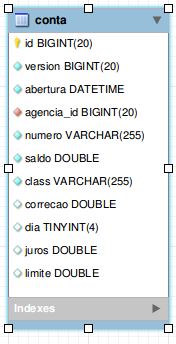
\includegraphics[height=7cm]{tablePerHierarchy}}
\qquad
\subfigure[{\it table-per-class}]{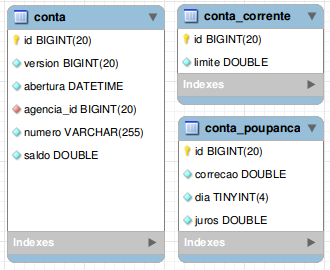
\includegraphics[height=5cm]{tablePerClass}}
\caption{GORM: Mapeamento de Hierarquia}
\label{gormFig}
\end{figure}

Porém, se o {\it default}  da estratégia de mapeamento {\it table-per-hierarchy}
não for  a mais adequada  para sua aplicação,  o desenvolvedor pode  utilizar um
mapeamento    alternativo     --    a    estratégia     {\it    table-per-class}
(Figura~\ref{gormFig}(b)). Nesse  caso, é  criada uma tabela  para a  classe pai
assim  como  para  cada  classe  filha.  Em nosso  exemplo,  a  estratégia  {\it
  table-per-class}  é habilitada  ao incluir  o trecho  apresentado a  seguir na
classe {\bf Conta} (pai da hierarquia).

\begin{cBox}
\begin{verbatim}
static mapping = {
    tablePerHierarchy false
}
\end{verbatim}
\end{cBox}

Pela  Figura~\ref{gormFig}(b), pode-se observar  que foi  criada uma  tabela que
armazena os atributos específicos de cada classe: {\bf Conta}) e suas subclasses
{\bf ContaCorrente} e {\bf ContaPoupanca}.

\newpage

\subsection{Classe de Domínio: Cliente}\label{secCliente}

\vspace{0.5cm}

A  classe  de  domínio  {\bf  Cliente}  representa  clientes  (correntistas)  de
instituições bancárias. Pelos requisitos da  aplicação, a classe {\bf Cliente} é
abstrata e portanto instâncias de {\bf Cliente} não podem ser criadas. Apenas de
suas  subclasses   {\bf  ClienteFisico}   e  {\bf  ClienteJuridico}   podem  ser
instanciadas.

Crie a  classe {\bf Cliente} do  pacote {\bf br.ufscar.dc.dsw}.   Na classe {\bf
  Cliente},  insira  os atributos  e  acrescente  as  suas validações,  conforme
apresentado no Código~\ref{codCliente}. 

\begin{lstlisting}[caption=Classe  de  domínio  {\bf  Cliente},  frame  =  trBL,
    float=htbp, label=codCliente] 
package br.ufscar.dc.dsw

abstract class Cliente {

    static hasMany = [contasCliente: ContaCliente]
    
    public static final String ATIVO = "Ativo"
    public static final String INATIVO = "Inativo"
    
    static constraints = {
        nome (blank: false, size: 1..30)
        endereco (nullable: false)
        dtMoradia (blank: false)
        status (blank: false, inList: [ATIVO, INATIVO])
    }
    
    static mapping = { 
        tablePerHierarchy false
    }
    
    String nome
    String status
    Endereco endereco
    Date dtMoradia
}
\end{lstlisting}

\hspace{1cm}\\
\noindent {\bf Observações:}
\hspace{1cm}\\

\begin{itemize}

\item A classe de domínio abstrata {\bf Cliente} possui os seguintes atributos:

\vspace{0.5cm}

\begin{itemize}

\item[$\diamond$] {\bf nome} -- que armazena o nome do cliente; 

\vspace{0.5cm}

\item[$\diamond$] {\bf status}  -- que armazena o {\it  status} do cliente: {\bf
  Ativo} ou {\bf Inativo};

\vspace{0.5cm}

\item[$\diamond$] {\bf endereco} -- que  armazena uma referência a uma instância
  da  classe  {\bf  Endereco}  (Seção~\ref{secEndereco}).  Esse  atributo  é  um
  mapeamento  unidirecional  entre  {\bf   Cliente}  e  {\bf  Endereco}.   Pelos
  requisitos  da aplicação,  não  há necessidade  de  implementar um  mapeamento
  bidirecional entre essas duas classes de domínio; e

\vspace{0.5cm}

\item[$\diamond$] {\bf dtMoradia} -- que  armazena desde quando o cliente reside
  no endereço armazenado no atributo {\bf endereco}.

\end{itemize}

\vspace{0.5cm}

\item O comando  {\bf static hasMany = [contasCliente:  ContaCliente]} na classe
  {\bf Cliente} e  o atributo {\bf cliente} na  classe {\bf ContaCliente}, foram
  utilizados  em conjunto  para implementar  um mapeamento  {\em um-para-muitos}
  entre essas classes.

\vspace{0.5cm}

\item Análoga  à classe {\bf  Conta}, a classe  de domínio {\bf  Cliente} também
  adota     a     estratégia     {\it     table-per-class}     no     mapeamento
  objeto-relacional. Portanto,  será criada uma  tabela para a classe  pai ({\bf
    Cliente})  assim  como  para  cada  subclasse: {\bf  ClienteFisico}  e  {\bf
    ClienteJuridico}.

\end{itemize}

\newpage

\subsection{Classe de Domínio: ClienteFisico}\label{secClienteFisico}

\vspace{0.5cm}

A classe de domínio {\bf  ClienteFisico}, subclasse de {\bf Cliente}, representa
clientes físicos  de instituições bancárias. Os  atributos {\bf rg}  e {\bf CPF}
armazenam respectivamente a  identidade e o número do  Cadastro de Pessoa Física
desses clientes.  

Crie  a classe  {\bf ClienteFisico}  do pacote  {\bf br.ufscar.dc.dsw}.   Abra a
classe {\bf ClienteFisico}, insira os atributos e acrescente as suas validações,
conforme  apresentado   no  Código~\ref{codClienteFisico}.  Salienta-se   que  a
validação do  atributo {\bf  CPF} utiliza a  restrição {\bf cpf:  true} definida
pelo {\it plugin} {\bf br-validation} instalado na Seção~\ref{secPlugins}. 

\begin{lstlisting}[caption=Classe de domínio  {\bf ClienteFisico}, frame = trBL,
    float=htbp, label=codClienteFisico] 
package br.ufscar.dc.dsw

class ClienteFisico extends Cliente{
    
    static constraints = {
        nome (blank: false, size: 1..30)
        rg (blank: false, size: 1..12)
        CPF (blank: false, unique:true, cpf: true, size: 14..14)
        endereco (nullable: false)
        dtMoradia (blank: false)
        status (blank: false, inList: [ATIVO, INATIVO])
    }
    
    String rg    
    String CPF
    
    String toString() {
        return CPF
    }
}
\end{lstlisting}

\subsection{Classe de Domínio: ClienteJuridico}\label{secClienteJuridico}

\vspace{0.5cm}

A  classe  de  domínio   {\bf  ClienteJurídico},  subclasse  de  {\bf  Cliente},
representa clientes  jurídicos de instituições bancárias. O  atributo {\bf CNPJ}
armazena o número do Cadastro Nacional de Pessoas Jurídicas desses clientes. 

Crie a  classe {\bf ClienteJuridico}  do pacote {\bf br.ufscar.dc.dsw}.   Abra a
classe  {\bf  ClienteJuridico},  insira   os  atributos  e  acrescente  as  suas
validações,    conforme    apresentado    no    Código~\ref{codClienteJuridico}.
Salienta-se  que a validação  do atributo  {\bf CNPJ}  utiliza a  restrição {\bf
  cnpj:  true}  definida pelo  {\it  plugin}  {\bf  br-validation} instalado  na
Seção~\ref{secPlugins}. 

\begin{lstlisting}[caption=Classe  de  domínio  {\bf ClienteJuridico},  frame  =
    trBL, float=htbp, label=codClienteJuridico] 
package br.ufscar.dc.dsw

class ClienteJuridico extends Cliente{
    
    static constraints = {
        nome (blank: false, size: 1..30)
        CNPJ (blank: false, unique:true, cnpj: true, size: 18..18)
        endereco (nullable: false)
        dtMoradia (blank: false)
        status (blank: false, inList: [ATIVO, INATIVO])
    }
    
    String CNPJ
    
    String toString() {
        return CNPJ
    }
}
\end{lstlisting}

\newpage

\section{Scaffolding}\index{Scaffolding}\label{Scaffolding}
\index{Modelo-Visão-Controlador (MVC)!Controlador}
\index{Modelo-Visão-Controlador (MVC)!Visão}

Uma  vez  que  as  classes  de   domínio  estão  criadas,  é  preciso  criar  os
controladores e as  visões relacionados a essas classes  de domínio.  Na geração
de tais artefatos de software será utilizada a abordagem {\it scaffolding} que é
um termo cunhado  pelo framework Rails e adotado pelo Grails  para a geração dos
artefatos (controladores, visões, etc.)  que implementam as operações CRUD. Esse
termo  foi estendido  e atualmente  é possível  criar código  de  autenticação e
autorização,  testes  unitários, dentre  outras  operações.  Em  Grails, o  {\it
  scaffolding}  pode   ser  dinâmico  ou  estático.    Discutiremos  essas  duas
abordagens distintas nas próximas subseções.

\subsection{Scaffolding Dinâmico}\index{Scaffolding!Dinâmico}

\vspace{0.3cm}

No {\it scaffolding} dinâmico, as visões são geradas em tempo de execução.  Essa
abordagem  simplifica  o desenvolvimento,  pois  nenhum  código relacionado  aos
controladores e  visões precisa ser desenvolvido.  O  {\it scaffolding} dinâmico
pode servir  a vários propósitos,  por exemplo, é  bastante útil na  criação das
interfaces de  administração de uma  aplicação web. No  entanto, ele não  é útil
quando  a  equipe  web  deseja  personalizar o  sistema  para  seus  propósitos,
principalmente as visões geradas em tempo de execução. 

\vspace{0.3cm}

\begin{itemize}

\item  Para  criar  um  controlador  (empregando  {\it  scaffolding  dinâmico}),
  relacionado à classe  de domínio {\bf Transacao}, no  IDE GGTS: Selecione {\bf
    Grails     Tools}      $\Longrightarrow$     {\bf     Create     Controller}
  (Figura~\ref{novoControladorFig}).  

\vspace{0.3cm}

\item Digite {\bf br.ufscar.dc.dsw.Transacao} como o nome do controlador e clique
  em   {\bf   Finish}.   O   GGTS    IDE   executa   o   comando   {\bf   grails
    create-controller},  apresentando  a  saída  na  janela  {\bf  Console}.   O
  controlador  {\bf  TransacaoController.groovy}  é  criado  no  diretório  {\bf
    grails-app/controllers}. \index{Comandos!grails create-controller}

\vspace{0.3cm}

\item  Abra  o controlador  {\bf  TransacaoController}  e implemente-o  conforme
  apresentado no Código~\ref{codTransacaoController}.

\end{itemize}

\vspace{0.5cm}

\begin{figure}[htbp]
\centering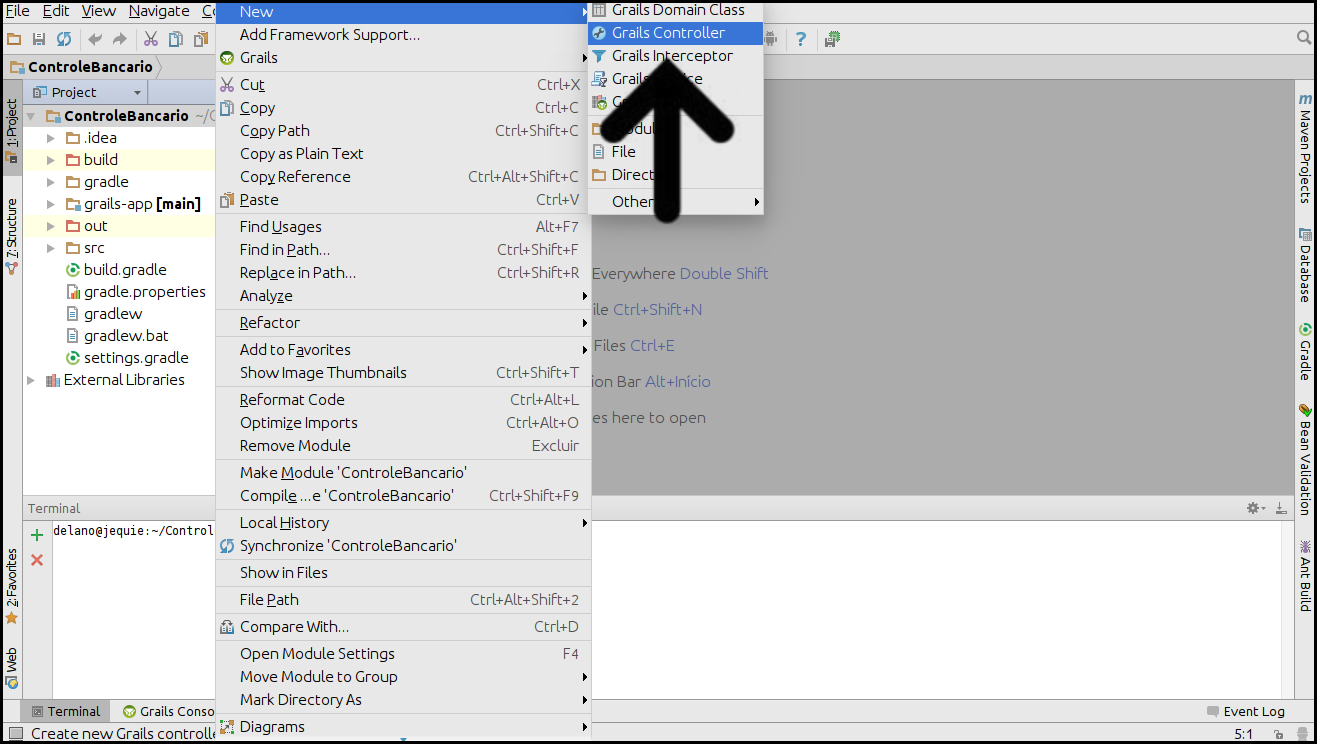
\includegraphics[width=13cm]{novoControlador}
\caption{Criação do controlador ({\it scaffolding} dinâmico).}
\label{novoControladorFig}
\end{figure}

\begin{lstlisting}[caption=Controlador {\bf TransacaoController (1)}, frame =
    trBL, float=htbp, label=codTransacaoController] 
package br.ufscar.dc.dsw

class TransacaoController {
    
    static scaffold = true

}
\end{lstlisting}

\subsection{Scaffolding Estático}\index{Scaffolding!Estático}\label{secEstatico} 

\vspace{0.5cm}

O {\it scaffolding}  estático produz, a partir de {\it  templates}, o código dos
controladores e visões que podem ser personalizados pela equipe web.  

Levando  em  consideração  esses  aspectos,  nesse  tutorial  adotou-se  o  {\it
  scaffolding} estático,  pois algumas customizações nos  controladores e visões
serão necessárias no desenvolvimento da aplicação {\bf ControleBancario}.

\begin{itemize}

\vspace{0.2cm}

\item  Para criar  um  controlador  e as  visões  (empregando {\it  scaffolding}
  estático) relacionado à classe de  domínio {\bf Transacao}, no GGTS: Selecione
  {\bf Grails Tools} $\Longrightarrow$ {\bf Grails Command Wizard}.  Digite {\bf
    generate-all}  como o  nome do  comando  a ser  executado e  clique em  {\bf
    Next}. Digite {\bf  Transacao} como o parâmetro do comando  e clique em {\bf
    Next} (Figura~\ref{geraTudoFig}).  \index{Comandos!grails generate-all}

\vspace{0.2cm}

\item Digite {\bf br.ufscar.dc.dsw.Transacao} como o nome da classe
  de    domínio   e   clique    em   {\bf    Finish}.    O    controlador   {\bf
    TransacaoController.groovy}      é     criado     no      diretório     {\bf
    grails-app/controllers} e o corresponde conjunto de {\em Groovy Server Pages
    (GSPs)} no diretório {\bf grails-app/views/transacao}.

\end{itemize}

\vspace{0.5cm}

\begin{figure}[htbp]
\centering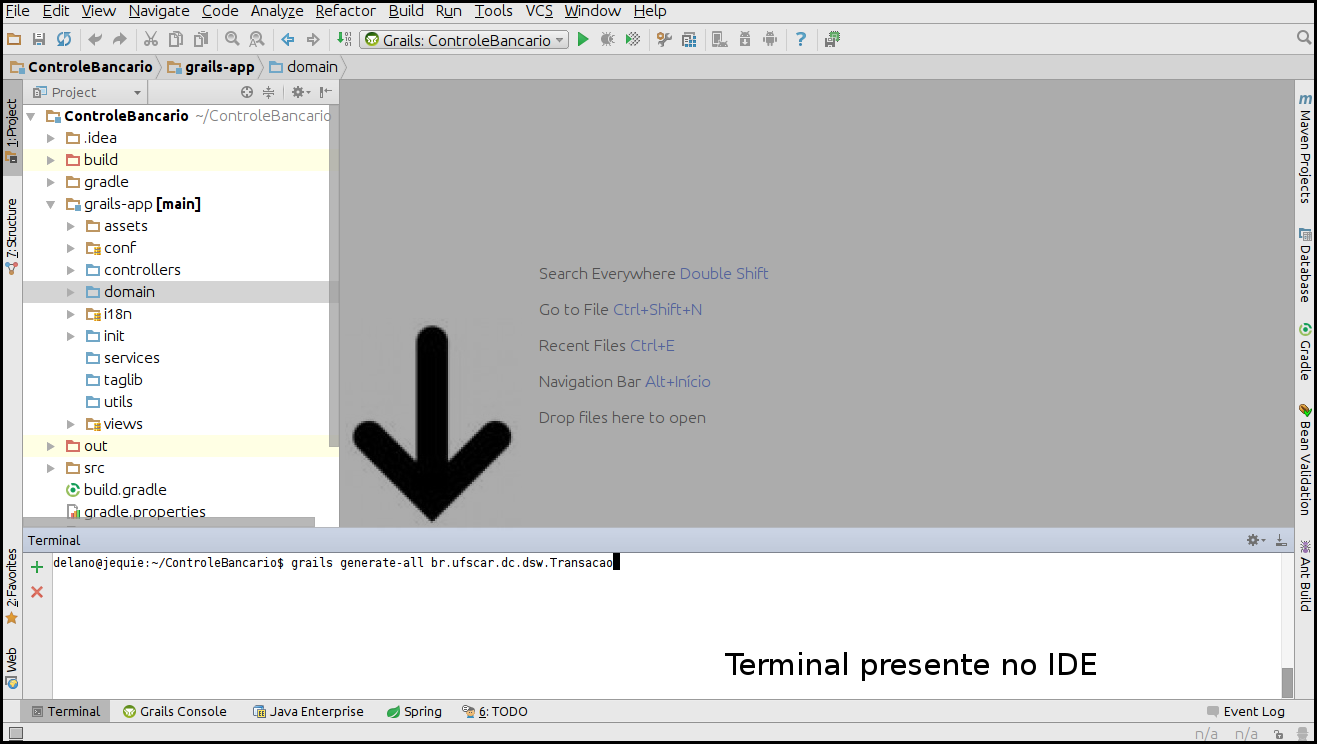
\includegraphics[width=12.5cm]{geraTudo}
\caption{Criação do controlador e das visões ({\it scaffolding} estático).}
\label{geraTudoFig}
\end{figure}

\vspace{0.5cm}

\noindent{\bf  Observação:} Para  cada método  correspondente a  uma ação  em um
controlador  é  criada  uma  correspondente  visão (arquivo  com  extensão  {\bf
  .gsp}). Por exemplo, a ação  {\bf show()} tem o correspondente {\bf show.gsp},
enquanto a ação {\bf create()} tem o correspondente {\bf create.gsp}. 

\newpage

Figura~\ref{scaffoldingFig} ilustra os controladores  e visões gerados pelo {\it
  scaffolding} da  classe de domínio {\bf Transacao}.   Destaca-se os benefícios
do paradigma {\it  Convention Over Configuration} em ação  em que nenhum arquivo
XML  é necessário para  associar esses  elementos. As  classes de  domínio estão
associadas   a   controladores  baseado   em   seus   respectivos  nomes   ({\bf
  Transacao.groovy}  $\rightarrow$ {\bf  TransacaoController.groovy}).  Conforme
já mencionado,  toda ação em um controlador  é associada a uma  visão baseada em
seu  nome ({\bf  index} $\rightarrow$  {\bf index.gsp}).   Desenvolvedores podem
configurar para  que o mapeamento seja  feito de outra maneira.   No entanto, na
maioria  das  vezes,   basta  seguir  a  convenção  e   a  aplicação  funcionará
corretamente      sem     maiores      configurações.      
\index{Convenção!{\it versus}~Configuração}

\vspace{0.5cm}

\begin{figure}[htbp]
\centering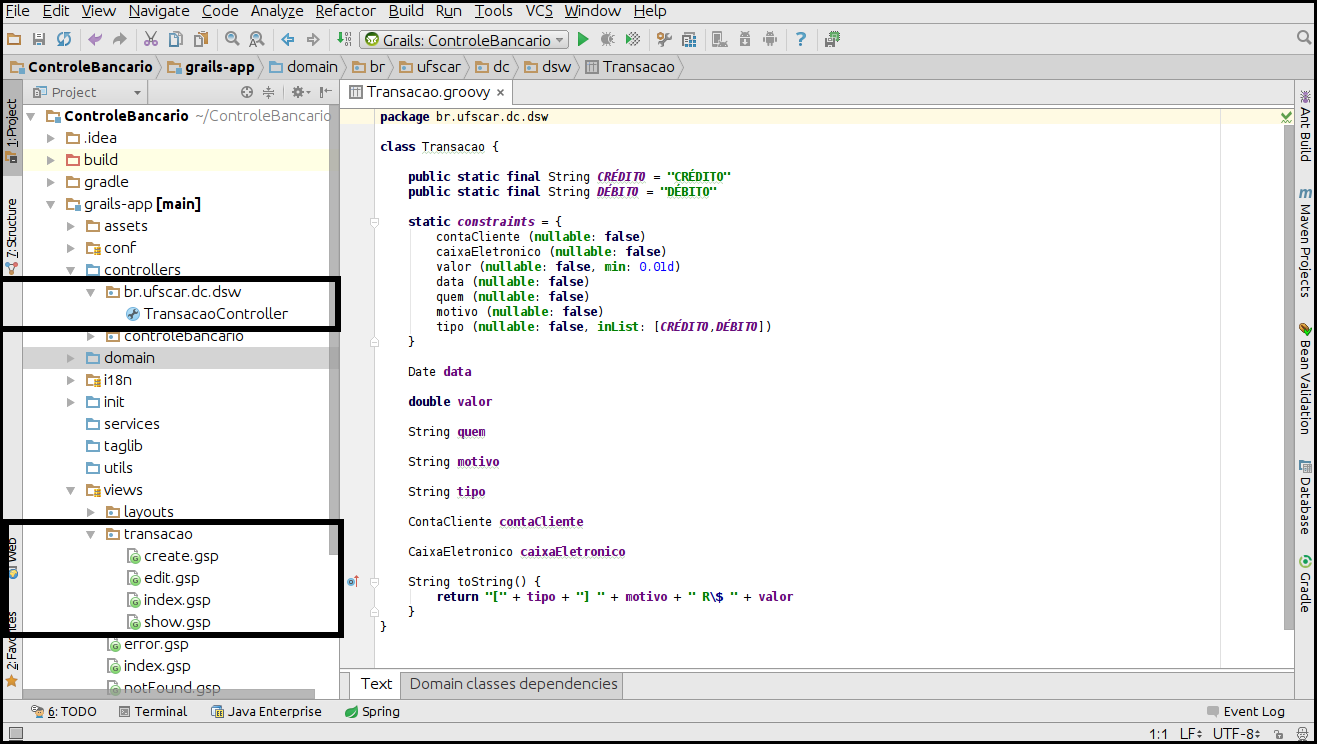
\includegraphics[width=14.5cm]{scaffolding}
\caption{Scaffolding estático das classes de domínio.}
\label{scaffoldingFig}
\end{figure}

\begin{remark}
Um bom exercício consiste em utilizar  o {\it scaffolding estático} para gerar o
controlador e as visões das demais classes de domínio.
\end{remark}

\begin{cBox}
Lembrar que não se gera os  controladores e visões para as classes {\bf Cliente}
e {\bf Conta}.  Essas classes são abstratas e não terão as operações de criação,
acesso, atualização e remoção (CRUD). 
\end{cBox}

\vspace{0.2cm}

\newpage

\subsection{Convenção na nomenclatura de URLs}\label{secURL}
\index{Convenção!Nomenclatura URL} 

\vspace{0.5cm}

Grails usa uma convenção (Figura~\ref{urlFig}) para automaticamente configurar o
caminho  para uma  ação em  particular. A  URL a  seguir pode  ser  entendida da
seguinte forma:

\begin{itemize}

\item ``{\it Execute a ação} {\bf show()} {\it do controlador} {\bf transacao} –
  {\it um dos controladores  da aplicação} {\bf ControleBancario} {\it hospedada
    na porta 8080 do servidor} {\bf localhost}''. 

\end{itemize}

\begin{figure}[htbp]
\centering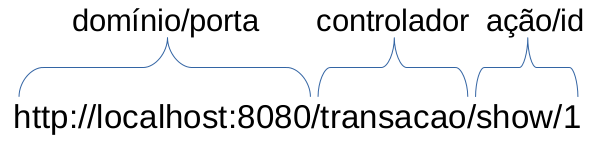
\includegraphics[width=10cm]{url}
\caption{Convenção na nomenclatura de URLs.}
\label{urlFig}
\end{figure}

A  regra principal  de roteamento  no Grails  forma URLs  segundo o  padrão {\bf
  /controlador/ação/id}, onde {\bf controlador}  é o controlador (da arquitetura
MVC) responsável  por atender  a requisição especificada  por aquela  {\it URL},
{\bf ação} é um método dentro do  controlador e {\bf id} é um parâmetro opcional
passado para identificar  um objeto qualquer sobre o qual  a ação será efetuada.
A  visão  associada  a essa  ação  geralmente  é  invocada (o  controlador  pode
redirecionar para outra visão).  

\begin{cBox}
Por exemplo, {\bf /transacao/edit/1} invoca a visão {\bf transacao/edit.gsp}. 
\end{cBox}

\subsection{Controlador: TransacaoController}\label{secTransacaoController}
\index{Modelo-Visão-Controlador (MVC)!Controlador}\

\begin{lstlisting}[caption=Controlador {\bf  TransacaoController}, frame = trBL,
    float=htbp, label=codTransacaoController2] 
@Transactional(readOnly = true) 
class TransacaoController { 
    static allowedMethods = [save: "POST", update: "PUT", delete: "DELETE"]

    def index(Integer max) {
        params.max = Math.min(max ?: 10, 100)
        respond Transacao.list(params), model:[transacaoInstanceCount: Transacao.count()]
    }

    def show(Transacao transacaoInstance) {
        respond transacaoInstance
    }

    def create() {
        respond new Transacao(params)
    }

    @Transactional
    def save(Transacao transacaoInstance) {
        if (transacaoInstance == null) {
            notFound()
            return
        }
        if (transacaoInstance.hasErrors()) {
            respond transacaoInstance.errors, view:'create'
            return
        }
        transacaoInstance.save flush:true
        request.withFormat {
            form {
                flash.message = message(code: 'default.created.message', args: [message(code: 'transacaoInstance.label', default: 'Transacao'), transacaoInstance.id])
                redirect transacaoInstance
            }
            '*' { respond transacaoInstance, [status: CREATED] }
        }
    }

    def edit(Transacao transacaoInstance) {
        respond transacaoInstance
    }

    @Transactional
    def update(Transacao transacaoInstance) {
        if (transacaoInstance == null) {
            notFound()
            return
        }
        if (transacaoInstance.hasErrors()) {
            respond transacaoInstance.errors, view:'edit'
            return
        }
        transacaoInstance.save flush:true
        request.withFormat {
            form {
                flash.message = message(code: 'default.updated.message', args: [message(code: 'Transacao.label', default: 'Transacao'), transacaoInstance.id])
                redirect transacaoInstance
            }
            '*'{ respond transacaoInstance, [status: OK] }
        }
    }

    @Transactional
    def delete(Transacao transacaoInstance) {
        if (transacaoInstance == null) {
            notFound()
            return
        }
        transacaoInstance.delete flush:true
        request.withFormat {
            form {
                flash.message = message(code: 'default.deleted.message', args: [message(code: 'Transacao.label', default: 'Transacao'), transacaoInstance.id])
                redirect action:"index", method:"GET"
            }
            '*'{ render status: NO_CONTENT }
        }
    }

    protected void notFound() {
        request.withFormat {
            form {
                flash.message = message(code: 'default.not.found.message', args: [message(code: 'transacaoInstance.label', default: 'Transacao'), params.id])
                redirect action: "index", method: "GET"
            }
            '*'{ render status: NOT_FOUND }
        }
    }
}
\end{lstlisting}

Para cada classes de entidade (classe  de domínio) persistente no banco de dados
tem-se  um controlador.  Por exemplo,  durante o  {\it scaffolding}  estático, o
controlador  {\bf  TransacaoController}  foi   gerado  com  as  seguintes  ações
(Código~\ref{codTransacaoController2}):

\begin{itemize}

\vspace{0.3cm}

\item   A  ação  {\bf   index()}  é   responsável  por   retornar  a   lista  de
  instâncias. Essa lista é repassada  para visão {\bf index.gsp} que a apresenta
  em uma página HTML;

\vspace{0.3cm}

\item  A ação  {\bf  show()} é  responsável  por retornar  os  atributos de  uma
  instância.   Essa instância  é repassada  para a  visão {\bf  show.gsp}  que a
  apresenta em uma página HTML;

\vspace{0.3cm}

\item  A  ação {\bf  create()}  é  responsável por  criar  uma  instância que  é
  repassada (retornada) para a visão  {\bf create.gsp} (uma página que contém um
  formulário HTML);

\vspace{0.3cm}

\item Quando  o formulário é  submetido, a ação  {\bf save()} valida os  dados e
  caso, tenha sucesso, grava a instância  no banco de dados e redireciona para a
  ação {\bf  show()}.  Por outro  lado, se os  dados são inválidos, a  ação {\bf
    save()}  renderiza a  visão {\bf  create.gsp} novamente  para que  o usuário
  corriga os erros encontrados na validação;

\vspace{0.3cm}

\item  A ação  {\bf edit()}  é  responsável por  recuperar uma  instância a  ser
  atualizada  posteriormente.  A  instância recuperada  é  repassada (retornada)
  para a visão {\bf edit.gsp} (uma página que contém um formulário HTML);

\vspace{0.3cm}

\item Quanto o formulário é submetido  o método {\bf update()} valida os dados e
  caso, tenha sucesso, atualiza a instância no banco de dados e redireciona para
  a ação {\bf show()}.   Por outro lado, se os dados são  inválidos, a ação {\bf
    update()}  renderiza a  visão {\bf  edit.gsp} novamente  para que  o usuário
  corriga os erros encontrados na validação; e

\vspace{0.3cm}

\item Por  fim, a  ação {\bf delete()}  remove uma  instância do banco  de dados
  através  da invocação  do método  {\bf delete  (flush:true)} no  objeto  a ser
  removido.

\end{itemize}

\vspace{0.3cm}

Seguem alguns detalhes importantes:

\vspace{0.3cm}

\begin{cBox}
\begin{small}
{\bf Três  Rs:} Em Grails,  ações normalmente terminam  em uma das  três formas,
iniciadas com a letra R.

\vspace{0.3cm}
\noindent{\bf Redirecionamento}  -- a ação  solicita que o pedido  seja atendido
por uma outra ação.

\vspace{0.3cm}
\noindent{\bf Renderização}  -- envia algum conteúdo (texto  simples, XML, JSON,
HTML, etc) para ser renderizado pelo navegador.

\vspace{0.3cm}
\noindent{\bf Retorno} --  o retorno geralmente é realizado  de forma explícita.
Outras vezes  o retorno  é implícito, como  vemos no  caso de {\bf  index()} que
retorna uma lista de transações e o tamanho da lista de transações.  
\end{small}
\end{cBox}

\subsection{{\it Groovy Server Pages (GSPs)}}
\index{Modelo-Visão-Controlador (MVC)!Visão}

\vspace{0.3cm}

Durante   o   {\it  scaffolding}   estático,   as   visões  relacionadas   ({\bf
  grails-app/views/transacao})  ao controlador  {\bf  TransacaoController} foram
criadas.  Essas  visões são  {\it  Groovy Server  Pages  (GSPs)}  que podem  ser
definidas  como um  arquivo  HTML básico  que  contêm alguma  {\it tags}  Grails
(elementos {\bf <g:  ..  />}).  Para desenvolvedores Java,  as {\it tags} Grails
são semelhantes às {\it tags}  disponíveis na {\bf JavaServer Pages Standard Tag
  Libraries}
(JSTL)\footnote{\url{http://www.oracle.com/technetwork/java/index-jsp-135995.html}}

Uma característica importante de GSPs é o {\it data-binding} entre o modelo e as
variáveis acessíveis pela visão durante a renderização das páginas HTML.  Assim,
um modelo é  um mapa (chave, valor)  que a visão utiliza. Por  exemplo, o trecho
apresentado no Código~\ref{codIndex} (visão  {\bf index.gsp}) tem acesso a lista
de  transações  (variável {\bf  transacaoInstanceList})  e  o  tamanho da  lista
(variável  {\bf  transacaoInstanceCount})  que  são retornados  pela  ação  {\bf
  index()} -- Código~\ref{codTransacaoController2}, linha 7.

\begin{lstlisting}[caption=Visão    {\bf    transacao/index.gsp},    frame=trBL,
    float=htbp, label=codIndex] 
<table>
	<thead>
		<tr>
			<th><g:message code="transacao.contaCliente.label" default="Conta Cliente" /></th>
			<th><g:message code="transacao.caixaEletronico.label" default="Caixa Eletronico" /></th>
			<g:sortableColumn property="valor" title="${message(code: 'transacao.valor.label', default: 'Valor')}" />
			<g:sortableColumn property="data" title="${message(code: 'transacao.data.label', default: 'Data')}" />
			<g:sortableColumn property="quem" title="${message(code: 'transacao.quem.label', default: 'Quem')}" />
			<g:sortableColumn property="motivo" title="${message(code: 'transacao.motivo.label', default: 'Motivo')}" />
		</tr>
	</thead>
	<tbody>
		<g:each in="${transacaoInstanceList}" status="i" var="transacaoInstance">
			<tr class="${(i % 2) == 0 ? 'even' : 'odd'}">
			  <td><g:link action="show" id="${transacaoInstance.id}">${fieldValue(bean: transacaoInstance, field: "contaCliente")}</g:link></td>
			  <td>${fieldValue(bean: transacaoInstance, field: "caixaEletronico")}</td>
			  <td>${fieldValue(bean: transacaoInstance, field: "valor")}</td>
			  <td><g:formatDate date="${transacaoInstance.data}" /></td>
			  <td>${fieldValue(bean: transacaoInstance, field: "quem")}</td>
			  <td>${fieldValue(bean: transacaoInstance, field: "motivo")}</td>
			</tr>
		</g:each>
	</tbody>
</table>
<div class="pagination">
	<g:paginate total="${transacaoInstanceCount ?: 0}" />
</div> 
\end{lstlisting}

\noindent O  {\it data-binding}  é realizado através  da utilização da  GSP {\it
  Expression Language  (EL)} que  facilita o acesso  aos modelos através  de uma
sintaxe simples  tais como {\bf \$\{transacaoInstanceCount\}}  para uma variável
simples ou {\bf \$\{transacaoInstance.data\}}  para um atributo de uma instância
de objeto.

\vspace{0.2cm}

Seguem-se as descrições de algumas {\it tags} GSP:

\vspace{0.2cm}

\begin{cBox}
\begin{itemize}

\item A tag {\bf <g:each>} itera  sobre a lista de transações, apresentando essa
  lista em uma tabela HTML. Cada elemento da lista é armazenado na variável {\bf
    transacaoInstance}.  

\vspace{0.2cm}

\item   A   expressão   {\bf  \$\{fieldValue(bean:   transacaoInstance,   field:
  "valor")\}} acessa o valor do  atributo {\bf valor} de cada transação presente
  na lista.  

\vspace{0.2cm}

\item      A     tag      {\bf     <g:link      action="show"     \hspace{0.2cm}
  id="\$\{transacaoInstance.id\}"  \hspace{0.1cm}>} cria  um {\it  link}  para a
  ação  {\bf   show}  do  controlador   atual  (no  caso,  o   controlador  {\bf
    TransacaoController}).  
\end{itemize}

\end{cBox}

\section{Executando a aplicação}\index{Bootstrap}

\vspace{0.5cm}

Após gerar  o CRUD das  entidades, através do  {\it scaffolding} estático  ou do
{\it  scaffolding} dinâmico,  a aplicação  pode ser  executada. Porém,  antes de
executar a  aplicação as  instâncias das entidades  podem ser criadas.  No caso,
serão  criados  instâncias  das  entidades  ({\bf Estado},  {\bf  Cidade},  {\bf
  Endereco}, etc) na classe  {\bf BootStrap.groovy} que encontra-se no diretório
{\bf grails-app/conf}. Essa classe é executada durante o {\it boot} da aplicação
e  serve, entre  outros propósitos,  para inicializar  a aplicação  por exemplo,
criando algumas instâncias de objetos.

A   implementação   da  classe   {\bf   BootStrap.groovy}   é  apresentado   nos
Códigos~\ref{codBootStrap1}~a~\ref{codBootStrap5}.   O   trecho  apresentado  no
Código~\ref{codBootStrap1}, popula  instâncias das  classes {\bf Estado}  e {\bf
  Cidade}.

\begin{lstlisting}[caption={\bf BootStrap.groovy (1)}, frame = trBL, float=htbp,
    label=codBootStrap1] 
import br.ufscar.dc.dsw.Agencia
import br.ufscar.dc.dsw.Banco
import br.ufscar.dc.dsw.CaixaEletronico
import br.ufscar.dc.dsw.Cidade
import br.ufscar.dc.dsw.Cliente
import br.ufscar.dc.dsw.ClienteFisico
import br.ufscar.dc.dsw.ClienteJuridico
import br.ufscar.dc.dsw.ContaCliente
import br.ufscar.dc.dsw.ContaCorrente
import br.ufscar.dc.dsw.ContaPoupanca
import br.ufscar.dc.dsw.Endereco
import br.ufscar.dc.dsw.Estado
import br.ufscar.dc.dsw.Gerente
import br.ufscar.dc.dsw.Transacao
class BootStrap {

    def init = { servletContext ->       

        def sp = new Estado(sigla: 'SP', nome: 'S^ã^o Paulo')
        sp.save()
        if (sp.hasErrors()) {
            println sp.errors
        }
        
        print 'populando estados - ok'
        
        def sanca = new Cidade(nome: 'S^ã^o Carlos', estado: sp)        
        sanca.save()
        if (sanca.hasErrors()) {
            println sanca.errors
        }
        
        def sampa = new Cidade(nome: 'S^ã^o Paulo', estado: sp)
        sampa.save()
        if (sampa.hasErrors()) {
            println sampa.errors
        }
        
        print 'populando cidades - ok'
\end{lstlisting}

\newpage

O  trecho  apresentado  no  Código~\ref{codBootStrap2},  popula  instâncias  das
classes {\bf Endereco}, {\bf Banco} e {\bf Agencia}.

\begin{lstlisting}[caption={\bf BootStrap.groovy (2)}, frame = trBL, float=htbp,
    label=codBootStrap2] 
        def end1 = new Endereco(logradouro: 'R. Conde do Pinhal', numero: 1909, 
            bairro: 'Centro', CEP: '13560-648', cidade: sanca)
        end1.save()
        if (end1.hasErrors()) {
            println end1.errors
        }
        
        def end2 = new Endereco(logradouro: 'R. Treze de Maio', numero: 1930, 
            bairro: 'Centro', CEP: '13560-647', cidade: sanca)
        end2.save()
        if (end2.hasErrors()) {
            println end2.errors
        }
        
        def end3 = new Endereco(logradouro: 'R. Nilton Coelho de Andrade',
            numero: 772, bairro: 'Vila Maria', CEP:'03092-324', cidade: sampa)        
        end3.save()
        if (end3.hasErrors()) {
            println end3.errors
        }
        
        def end4 = new Endereco(logradouro: 'R. Humberto Manelli', numero: 50, 
            complemento: 'Apto 31', bairro: 'Jardim Gibertoni', 
            CEP:'13562-420', cidade: sanca)
        
        end4.save()
        if (end4.hasErrors()) {
            println end4.errors
        }
        
        print 'populando endere^ç^os - ok'
        
        def bb = new Banco(numero: 1, nome: 'Banco do Brasil', 
            CNPJ: '00.000.000/0001-91')
        
        bb.save()
        if (bb.hasErrors()) {
            println bb.errors
        }
        
        def santander = new Banco(numero: 33, nome: 'Santander', 
            CNPJ: '90.400.888/0001-42')
        
        santander.save()
        if (santander.hasErrors()) {
            println santander.errors
        }

        print 'populando bancos - ok'
        
        def agencia1 = new Agencia(numero: 1888, nome: 'Conde do Pinhal', 
            endereco: end1, banco: bb)
        
        agencia1.save()
        if (agencia1.hasErrors()) {
            println agencia1.errors
        }
        
        def agencia2 = new Agencia(numero: 24, nome: 'Treze de Maio', 
            endereco: end2, banco: santander)
        
        agencia2.save()
        if (agencia2.hasErrors()) {
            println agencia2.errors
        }
        
        print 'populando ag^ê^ncias - ok'
\end{lstlisting}

\newpage

O  trecho  apresentado  no  Código~\ref{codBootStrap3},  popula  instâncias  das
classes  {\bf  Gerente},  {\bf  CaixaEletronico},  {\bf  ClienteFisico}  e  {\bf
  ClienteJuridico}. 

\begin{lstlisting}[caption={\bf BootStrap.groovy (3)}, frame = trBL, float=htbp,
    label=codBootStrap3] 
        def gerente1 = new Gerente(nome: 'Carlos da Silva', rg: '1234 SSP/SP',
            CPF: '129.304.458-07', agencia: agencia1
        )
    
        gerente1.save()
        if (gerente1.hasErrors()) {
            println gerente1.errors
        }
        
        def gerente2 = new Gerente(nome: 'Maria Jos^é^', rg: '3467 SSP/RJ',
            CPF: '018.990.444-50', agencia: agencia2
        )
    
        gerente2.save()
        if (gerente2.hasErrors()) {
            println gerente2.errors
        }
        
        print 'populando gerentes - ok'
        
        def caixa1 = new CaixaEletronico(banco: bb, endereco: end1)
        
        caixa1.save()
        if (caixa1.hasErrors()) {
            println agencia1.errors
        }
        
        def caixa2 = new CaixaEletronico(banco: santander, endereco: end2)
        
        caixa2.save()
        if (caixa2.hasErrors()) {
            println agencia1.errors
        }
        
        print 'populando caixas eletr^ô^nicos - ok'
        
        def cliFisico = new ClienteFisico(nome: 'Fulano de Tal', 
            rg: '13567 SSP/SP', CPF: '018.990.444-50', endereco: end4,
            dtMoradia: new Date(), status: Cliente.ATIVO) 
        
        cliFisico.save()
        if (cliFisico.hasErrors()) {
            println cliFisico.errors
        }
        
        print 'populando clientes f^í^sicos - ok'
                
        def cliJuridico = new ClienteJuridico(nome: 'Via^çã^o Cometa S/A', 
            CNPJ: '61.084.018/0001-03', endereco: end3,
            dtMoradia: new Date(), status: Cliente.ATIVO) 
        
        cliJuridico.save()
        if (cliJuridico.hasErrors()) {
            println cliJuridico.errors
        }
        
        print 'populando clientes jur^í^dicos - ok'
\end{lstlisting}

\newpage

O  trecho  apresentado  no  Código~\ref{codBootStrap4},  popula  instâncias  das
classes  {\bf ContaCorrente},  {\bf ContaPoupanca}  e {\bf  Transacao}. Conforme
pode-se observar,  as instâncias da  classe {\bf Transacao}  criadas representam
depósitos e saques.
  
\begin{lstlisting}[caption={\bf BootStrap.groovy (4)}, frame = trBL, float=htbp,
    label=codBootStrap4] 
        def corrente = new ContaCorrente(agencia: agencia1, 
            numero: '010414688', saldo: 1000.56d, limite: 500.00d,
            abertura: new Date()
        )
    
        corrente.save()
        if (corrente.hasErrors()) {
            println corrente.errors
        }

        def contaCli1 = new ContaCliente(conta: corrente, 
            cliente: cliJuridico, titular: true
        )
    
        contaCli1.save()
        if (contaCli1.hasErrors()) {
            println contaCli1.errors
        }
        
        print 'populando contas correntes (associado ao cliente jur^í^dico) - ok'
                
        def poupanca = new ContaPoupanca(agencia: agencia2, 
            numero: '261327', saldo: 10000.56d, juros: 0.50d,
            correcao: 1.20d, dia: 23, abertura: new Date()
        )
    
        poupanca.save()
        if (poupanca.hasErrors()) {
            println poupanca.errors
        }


        def contaCli2 = new ContaCliente(conta: poupanca, 
            cliente: cliFisico, titular: true
        )
    
        contaCli2.save()
        if (contaCli2.hasErrors()) {
            println contaCli2.errors
        }
        
        print 'populando contas poupan^ç^as (associado ao cliente f^í^sico) - ok'
        
        def deposito = new Transacao(contaCliente: contaCli2, caixaEletronico: caixa2, 
            valor: 50d, data: new Date(), quem: 'Pr^ó^prio', motivo: 'Dep^ó^sito',
            tipo: Transacao.CR^É^DITO
        )
        
        deposito.save()
        if (deposito.hasErrors()) {
            println deposito.errors
        }
        
        print 'populando depositos - ok'
        
        def saque = new Transacao(contaCliente: contaCli1, caixaEletronico: caixa1, 
            valor: 100d, data: new Date(), quem: 'Pr^ó^prio', motivo: 'Saque', 
            tipo: Transacao.D^É^BITO)
        
        saque.save()
        if (saque.hasErrors()) {
            println saque.errors
        }
        
        print 'populando saques - ok'
\end{lstlisting}

\newpage

E por fim, o trecho apresentado no Código~\ref{codBootStrap5}, popula instâncias
da classe  {\bf Transacao}. Conforme  pode-se observar, as instâncias  da classe
{\bf Transacao} criadas representam transferências bancárias.

\begin{lstlisting}[caption={\bf BootStrap.groovy (5)}, frame = trBL, float=htbp,
    label=codBootStrap5] 
        def transf1 = new Transacao(contaCliente: contaCli1, 
            caixaEletronico: caixa2, valor: 25d, data: new Date(),
            quem: 'Pr^ó^prio', motivo: 'Transfer^ê^ncia', tipo: Transacao.D^É^BITO)
        
        def transf2 = new Transacao(contaCliente: contaCli2, 
            caixaEletronico: caixa2, valor: 25d, data: new Date(),
            quem: 'Fulano de Tal', motivo: 'Transfer^ê^ncia', 
            tipo: Transacao.CR^É^DITO)
        
        transf1.save()
        if (transf1.hasErrors()) {
            println transf1.errors
        }
        
        transf2.save()
        if (transf2.hasErrors()) {
            println transf2.errors
        }
        
        print 'populando transferencias - ok'
    }

    def destroy = {
    }
}
\end{lstlisting}

\vspace{0.3cm}

Para executar  a aplicação,  clique no  botão direito do  mouse no  projeto {\bf
  ControleBancario}  e   escolha  {\bf  Run  As}   $\rightarrow$  {\bf  run-app}
(Figura~\ref{executarFig}).  A aplicação é implantada no servidor Web, como pode 
ser  visto na  janela {\bf  Console} do  IDE GGTS  IDE. Seguem-se  os principais
passos da execução: \index{Comandos!grails run-app}

\vspace{0.3cm}

\begin{itemize}

\item   A   URL  {\footnotesize\url{http://localhost:8080/ControleBancario}}   é
  impressa na  janela {\bf Console}.  Se o navegador não  abrir automaticamente,
  cole a  URL em um navegador e  a aplicação será acessada.  Os controladores da
  aplicação serão listados (Figura~\ref{executarFig}).

\end{itemize}

\vspace{0.2cm}

\begin{figure}[htbp]
\centering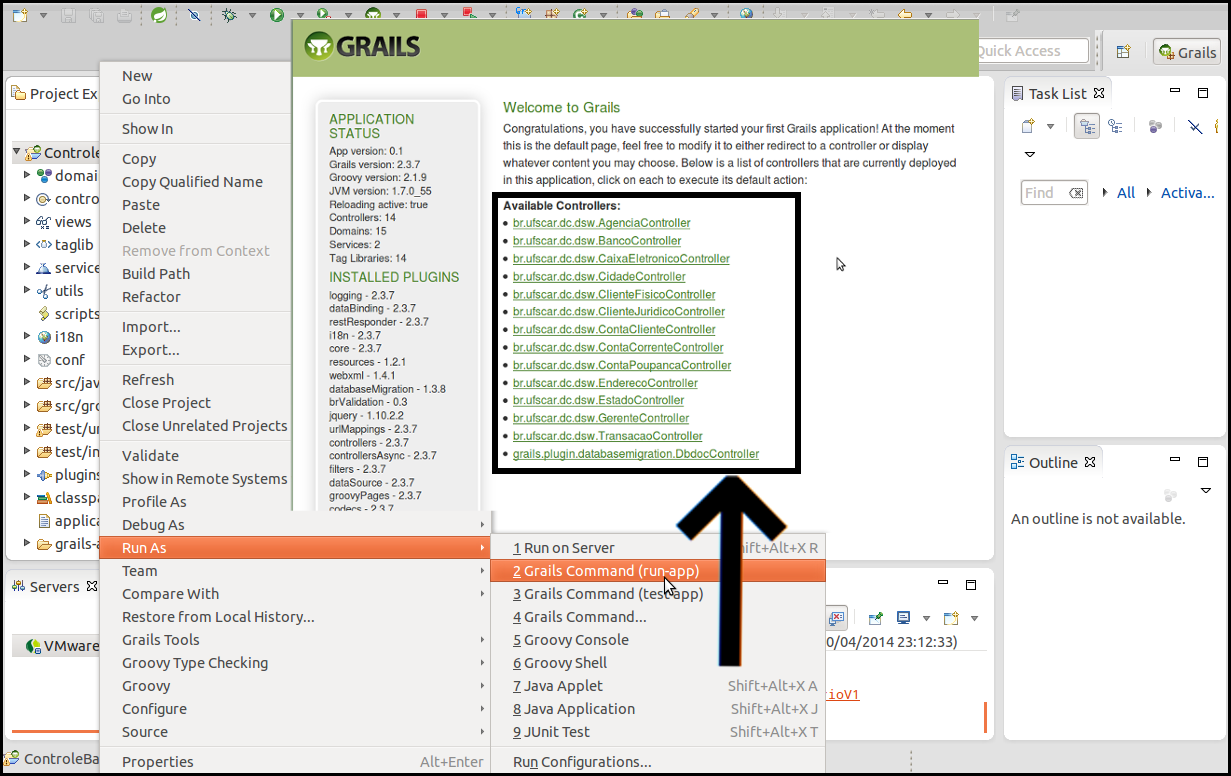
\includegraphics[width=14cm]{executar}
\caption{Execução da aplicação {\bf ControleBancario}}
\label{executarFig}
\end{figure}

\vspace{0.3cm}

\begin{itemize}

\item   Ao  clicar  no   link  {\bf   br.ufscar.dc.dsw.TransacaoController},  as
  transações  bancárias  inseridas  anteriormente ({\bf  BootStrap.groovy})  são
  apresentadas (Figura~\ref{listaTransacoesFig}). 

\end{itemize}

\begin{figure}[htbp]
\centering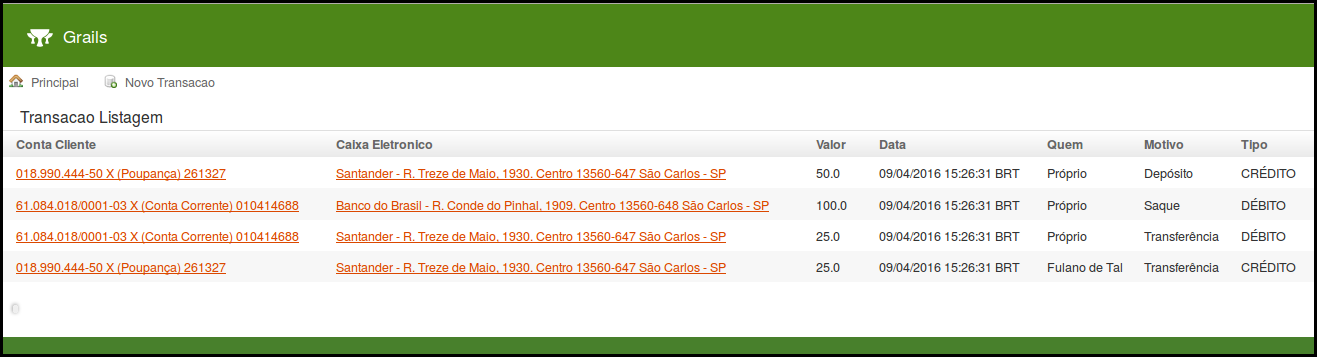
\includegraphics[width=11cm]{listaTransacoes}
\caption{Lista de transações bancárias}
\label{listaTransacoesFig}
\end{figure}

\vspace{0.2cm}

\begin{itemize}

\item Clique em {\bf Novo Transacao}  e crie uma nova transação bancária. Quando
  clicar em {\bf Criar}, observe que você poderá {\bf Editar} ou {\bf Remover} a
  transação. Por  fim, ao clicar em  {\bf Transacao Listagem}, a  nova entrada é
  apresentada na lista de transações (Figura~\ref{novaTransacaoFig}). 

 \end{itemize}

\begin{figure}[htbp]
\centering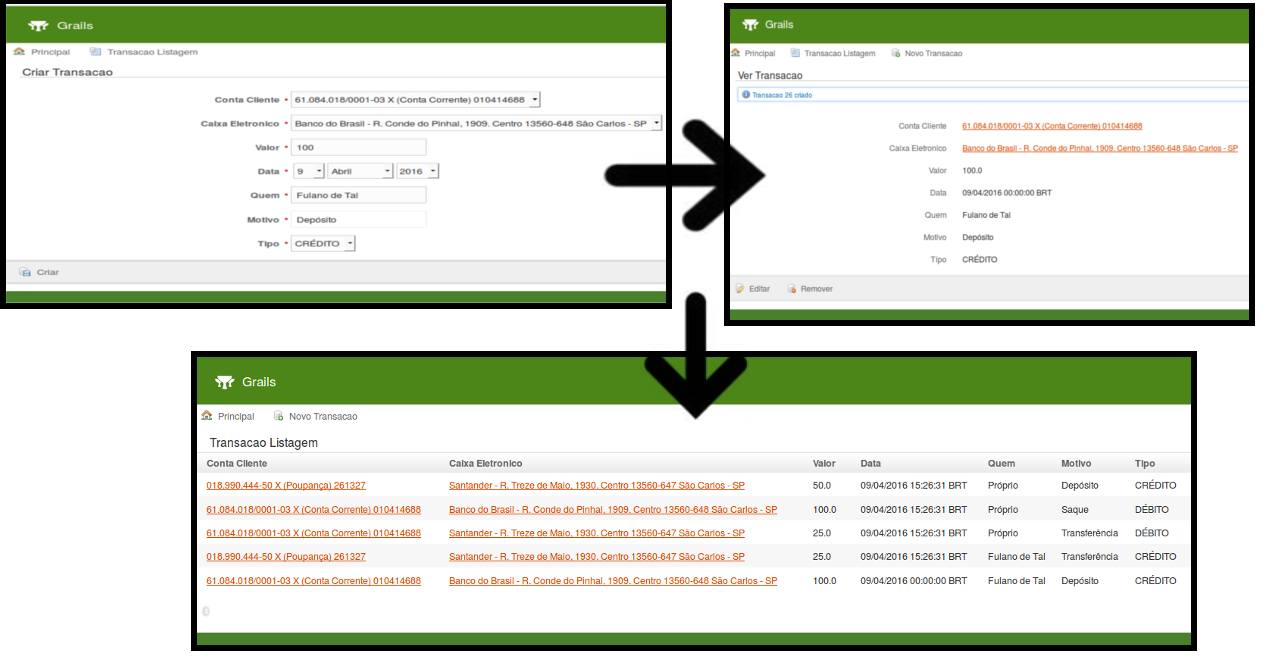
\includegraphics[width=13.4cm]{novaTransacao}
\caption{Criação de uma nova transação bancária}
\label{novaTransacaoFig}
\end{figure}

Salienta-se que para a criação das outras entidades da aplicação ({\bf Cliente},
{\bf Conta} e outros), os passos são análogos.  

\newpage

\begin{itemize}

\item Clique  em {\bf  Novo Transacao}  e crie uma  nova transação  bancária com
  valores  inválidos   (Figura~\ref{transacaoInvalidaFig}).   Verfica-se  que  a
  transação não foi criada, pois as validações de dados foram violadas. 

\end{itemize}

\begin{figure}[htbp]
\centering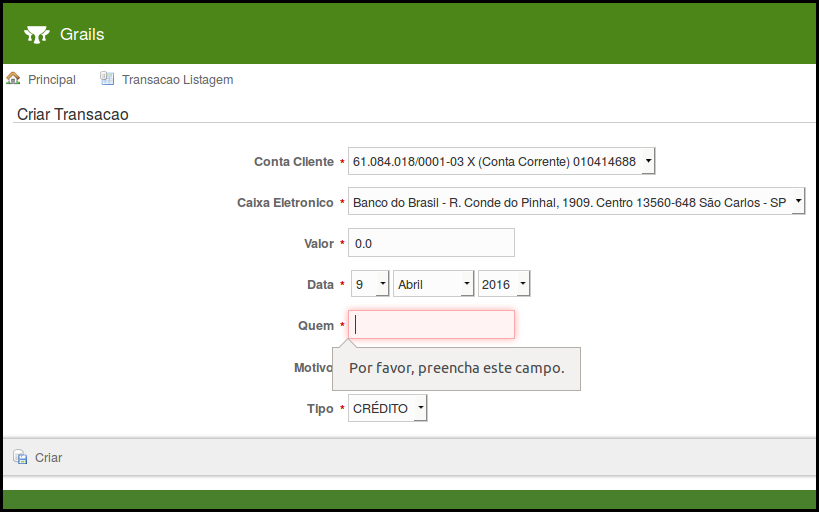
\includegraphics[width=12cm]{transacaoInvalida}
\caption{Criação de uma transação bancária com valores inválidos}
\label{transacaoInvalidaFig}
\end{figure}

\vspace{0.5cm}

\begin{remark}
Sugere-se, como aprendizado, executar os  demais controladores e verificar se as
demais funcionalidades da aplicação encontram-se funcionando corretamente.
\end{remark}

\section{Considerações finais}

\vspace{0.3cm}

Esse   capítulo  apresentou   uma  implementação   parcial  da   aplicação  {\bf
  ControleBancario}.         O        código-fonte        dessa        aplicação
({\footnotesize\texttt{ControleBancarioV1.zip}}) encontra-se  disponível no {\it
  Moodle}         do        curso,        localizado         no        endereço:
{\footnotesize\url{http://moodle.latosensu.dc.ufscar.br}}. Seguindo os passos do
tutorial   apresentado   obtem-se   esse   mesmo  código   da   aplicação   {\bf
  ControleBancario}.  

Dando continuidade ao desenvolvimento em Grails, o próximo capítulo apresenta a
implementação   de  novas   funcionalidades  no   contexto  da   aplicação  {\bf
  ControleBancario}.  




%-------------------------------------------------------------------------------
%	CAPÍTULO 3
%-------------------------------------------------------------------------------

\chapter{Controle Bancário: Versão 2}\label{autenticacao}

Neste  capítulo,   dando  continuidade   ao  desenvolvimento  em   Grails,  será
apresentado o  processo de desenvolvimento  da segunda versão da  aplicação {\bf
  ControleBancario}. Nessa versão são incorporadas as seguintes funcionalidades:

\begin{itemize}

\vspace{0.5cm}

\item Controle de acesso: autenticação e autorização de usuários;

\vspace{0.5cm}

\item  Internacionalização. Ou  seja,  personalizar o  conteúdo apresentado  nas
  visões (*.gsp) com base no {\it Locale} (idioma e região) dos usuários;

\vspace{0.5cm}

\item  Personalização dos  {\it  templates} utilizados  pelo  mecanismo de  {\it
  scaffolding} na geração dos controladores e visões;

\vspace{0.5cm}

\item Definição  de máscaras de entrada para  os atributos CEP, CNPJ,  e CPF das
  classes de domínio; e 

\vspace{0.5cm}

\item  Implementação de  uma biblioteca  de marca\footnote{Em  inglês:  {\it tag
    library.}} que apresenta informações relacionadas ao usuário logado. 

\end{itemize}

\section{Configuração da aplicação} 

\vspace{0.5cm}

\hyphenation{ControleBancario}

\noindent{\bf (a) Instalação de  plugins.}  Na implementação das funcionalidades
da aplicação {\bf ControleBancario}, discutidas nesse capítulo, será utilizado o
plugin Grails {\bf  spring-security} que auxilia a autenticação  dos usuários da
aplicação.\index{Plugins!spring-security} Conforme discutido anteriormente, para
instalar  o  plugin {\bf  spring-security}  adicione  uma  linha, descrevendo  a
dependência, no arquivo  {\bf build.gradle} conforme apresentado na  linha 50 do
Código~\ref{codBuildGradle2}.  

\newpage

\noindent{\bf (b)  Instalação de bibliotecas Javascript.}   Na implementação das
funcionalidades  discutidas nesse  capítulo, será  utilizada a  biblioteca: {\bf
  jquery.maskedinput.min.js}\footnote{\url{http://digitalbush.com/projects/masked-input-plugin}}. 
Dessa forma,  é necessário fazer  o {\it download}  desse arquivo e  copiá-lo no
diretório {\bf grails-app/assets/javascripts}.  

\vspace{0.5cm}

\noindent{\bf  (c)  Atualização  das   dependências.}   Por  fim,  é  necessário
atualizar    as    dependências    ({\it    plugins})    da    aplicação    {\bf
  ControleBancario}. Para tal,  no IDE IntelliJ: abra a  janela {\bf Terminal} e
execute  o  comando  {\bf  grails  compile}.  Esse  comando  compila  o  projeto
atualizando as dependências e instala os {\it plugins}, caso necessário. 
\index{Comandos!grails compile} 

\begin{lstlisting}[numbers=left, caption={\bf BuildConfig.groovy}, frame = trBL,
    float=htbp, label=codBuildGradle2]
buildscript {
    ext {
        grailsVersion = project.grailsVersion
    }
    repositories {
        mavenLocal()
        maven { url "https://repo.grails.org/grails/core" }
    }
    dependencies {
        classpath "org.grails:grails-gradle-plugin:$grailsVersion"
        classpath "com.bertramlabs.plugins:asset-pipeline-gradle:2.5.0"
        classpath "org.grails.plugins:hibernate4:5.0.2"
    }
}
version "0.1"
group "controlebancario"
apply plugin:"eclipse"
apply plugin:"idea"
apply plugin:"war"
apply plugin:"org.grails.grails-web"
apply plugin:"org.grails.grails-gsp"
apply plugin:"asset-pipeline"
ext {
    grailsVersion = project.grailsVersion
    gradleWrapperVersion = project.gradleWrapperVersion
}
repositories {
    mavenLocal()
    maven { url "https://repo.grails.org/grails/core" }
}
dependencyManagement {
    imports {
        mavenBom "org.grails:grails-bom:$grailsVersion"
    }
    applyMavenExclusions false
}
dependencies {
    compile "org.springframework.boot:spring-boot-starter-logging"
    compile "org.springframework.boot:spring-boot-autoconfigure"
    compile "org.grails:grails-core"
    compile "org.springframework.boot:spring-boot-starter-actuator"
    compile "org.springframework.boot:spring-boot-starter-tomcat"
    compile "org.grails:grails-dependencies"
    compile "org.grails:grails-web-boot"
    compile "org.grails.plugins:cache"
    compile "org.grails.plugins:scaffolding"
    compile "org.grails.plugins:hibernate4"
    compile "org.hibernate:hibernate-ehcache"
    compile "org.grails.plugins:br-validation:0.3"
    compile "org.grails.plugins:spring-security-core:3.0.4"
    console "org.grails:grails-console"
    profile "org.grails.profiles:web:3.1.4"
    runtime "org.grails.plugins:asset-pipeline"
    runtime "com.h2database:h2"
    runtime "org.postgresql:postgresql:9.3-1101-jdbc41"
    testCompile "org.grails:grails-plugin-testing"
    testCompile "org.grails.plugins:geb"
    testRuntime "org.seleniumhq.selenium:selenium-htmlunit-driver:2.47.1"
    testRuntime "net.sourceforge.htmlunit:htmlunit:2.18"
}
task wrapper(type: Wrapper) {
    gradleVersion = gradleWrapperVersion
}
assets {
    minifyJs = true
    minifyCss = true
}
\end{lstlisting}

\newpage

\section{Controle de Acesso}

\vspace{0.3cm}

Conforme dito,  a segunda versão  da aplicação {\bf ControleBancario}  utiliza o
{\it                                 plugin}                                {\bf
  spring-security-core}\footnote{\url{http://grails.org/plugin/spring-security-core}}
que          simplifica         a          integração          do         Spring
Security\footnote{\url{http://static.springsource.org/spring-security/site/index.html}}
em aplicações Grails. \index{Plugins!spring-security} 

\vspace{0.3cm}

Esse {\it plugin}  define uma série de comandos. Entre  esses podemos destacar o
comando {\bf s2-quickstart}  que cria tanto as classes  de domínio básicas tanto
os  controladores (e  suas  respectivas  visões) necessários  para  lidar com  a
autenticação de usuários. 

\vspace{0.3cm}

Portanto, o  primeiro passo  na implementação da  funcionalidade de  controle de
acesso é  a execução desse  comando.  Para tal,  no IDE IntelliJ: abra  a janela
{\bf Terminal}  e execute o  comando {\bf grails  s2-quickstart br.ufscar.dc.dsw
  Usuario Papel}.  Esse comando cria os seguintes artefatos:
\index{Comandos!grails s2-quickstart} 

\vspace{0.5cm}

\begin{itemize}

\item  {\bf br.ufscar.dc.dsw.Usuario}  -- classe  de domínio  que  representa os
  usuários autenticados. 

\vspace{0.3cm}

\item {\bf br.ufscar.dc.dsw.Papel} -- classe de domínio que representa os papéis
  que  os  usuários  podem  desempenhar.  Cada papel  possui  permissões  a  ele
  associadas.  

\vspace{0.5cm}

\item {\bf br.ufscar.dc.dsw.UsuarioPapel} --  classe de domínio que representa o
  relacionamento  muitos-para-muitos  entre  usuários  e papéis.   Ou  seja,  um
  usuário pode  desempenhar vários papeis e  um papel pode  ser desempenhado por
  vários usuários. 

\vspace{0.5cm}

\item {\bf LoginController} e {\bf LogoutController} (e suas respectivas visões)
  que  são  responsáveis  pelas operações  de  {\it  login}  e {\it  logout}  da
  aplicação.

\end{itemize}

\vspace{0.5cm}

A seguir, adicione  o seguinte trecho na classe de domínio  {\bf Usuario} -- pai
da  hierarquia de  usuários  da  aplicação {\bf  ControleBancario}.  Ou seja,  a
estratégia  de mapeamento  {\it table-per-hierarchy}  (Seção~\ref{secGORM}) será
desabilitada   e,  para   essa  hierarquia   de  classes,   a   estratégia  {\it
  table-per-class} será  utilizada.  Assim,  é criada uma  tabela para  a classe
{\bf Usuario} assim como para cada classe filha discutida nas próximas seções.

\vspace{0.5cm}

\begin{cBox}
\begin{small}
\begin{verbatim}
static mapping = {
    password column: '`password`'
    tablePerHierarchy false
}
\end{verbatim}
\end{small}
\end{cBox}

\vspace{0.5cm}

\hyphenation{LogoutController}

Por     fim,    adicione     o     seguinte    trecho     no    arquivo     {\bf
  conf/application.groovy}. Esse  comando habilita que  os comandos \texttt{HTTP
  POST}  e  \texttt{GET}  sejam  utilizados  para  invocar  o  controlador  {\bf
  LogoutController}  que  é  responsável   pela  operação  de  {\it  logout}  da
aplicação. Por {\it default}, apenas  o comando \texttt{POST} pode ser utilizado
para invocar o controlador {\bf LogoutController}. 

\vspace{0.5cm}

\begin{cBox}
\begin{small}
\begin{verbatim}
grails.plugin.springsecurity.logout.postOnly = false
\end{verbatim}
\end{small}
\end{cBox}

\newpage

\subsection{Classes de Domínio: Cliente, ClienteFisico, ClienteJuridico e Gerente}

Os    clientes   e   os    gerentes   serão    usuários   da    aplicação   {\bf
  ControleBancario}.  Ou  seja, as  classes  de  domínio  {\bf Cliente}  e  {\bf
  Gerente}   são  subclasses  da   classe  {\bf   Usuario}  definida   na  seção
anterior. Desde que  as classes {\bf ClienteFisico} e  {\bf ClienteJuridico} são
subclasses de {\bf Cliente}, estas também serão subclasses de {\bf Usuario}.

\vspace{0.2cm}

A classe {\bf Usuario} define dois atributos {\bf username} e {\bf password} que
são  responsáveis pelo  armazenamento do  {\it login}  e senha  dos  usuários da
aplicação.   Código~\ref{codUsuario}  mostra   as  alterações  na  implementação
das  classes {\bf Cliente},  {\bf ClienteFisico},  {\bf ClienteJuridico}  e {\bf
  Gerente}.   Pode-se  observar  que   na  implementação  dessas  classes  foram
incluídas  restrições   relacionadas  aos   atributos  {\bf  username}   e  {\bf
  password} definidos pela classe pai {\bf Usuario}. 

\begin{lstlisting}[caption=Usuários:   Clientes  e   Gerentes,  frame   =  trBL,
    float=htbp, label=codUsuario] 
abstract class Cliente extends Usuario {  
 
   static constraints = {
        username (blank: false, unique: true)
        password (password: true, blank: false)
        // demais restri^çõ^es
    }

    // atributos e m^é^todos da classe
}

class ClienteFisico extends Cliente {
    
    static constraints = {
        username (blank: false, unique: true)
        password (password: true, blank: false)
        // demais restri^çõ^es
    }
    
    // atributos e m^é^todos da classe
}

class ClienteJuridico extends Cliente {
    
    static constraints = {
        username (blank: false, unique: true)
        password (password: true, blank: false)
        // demais restri^çõ^es
    }
    
   // atributos e m^é^todos da classe
}

class Gerente extends Usuario {

    static constraints = {
        username (blank: false, unique: true)
        password (password: true, blank: false)
        // demais restri^çõ^es
    }
   
    // atributos e m^é^todos da classe
}
\end{lstlisting}

\section{Internacionalização}\label{I18n}
\index{Internacionalização~-~I18n}

Grails  apoia a internacionalização  (i18n). Ou  seja, com  o Grails  é possível
personalizar o conteúdo  que aparece em qualquer visão (*.gsp)  com base no {\it
  Locale} dos usuários. Para tirar  proveito do suporte a internacionalização em
Grails, a equipe  de desenvolvimento tem que criar {\it  message bundles} -- uma
para cada idioma  que a equipe deseja internacionalizar.   {\it Message bundles}
em  Grails  estão localizados  dentro  do diretório  {\bf  i18n}  e são  simples
arquivos de propriedades    Java/Groovy.     

\vspace{0.2cm}

Por padrão, Grails procura em  {\it messages.properties} para mensagens, a menos
que o  usuário tenha  especificado um  {\it Locale} em  específico. A  equipe de
desenvolvimento  pode criar  novas  {\it message  bundles} simplesmente  criando
novos  arquivos  de  propriedades  que   terminam  com  a  localidade  que  está
interessada.  Por exemplo, {\it messages\_pt\_BR.properties} para o Português do
Brasil (Figura~\ref{I18nFig}).

\begin{small}
\begin{cBox}
Um objeto {\it Locale} representa  uma região geográfica específica, político ou
cultural. Uma  operação que requer uma  localidade para executar a  sua tarefa é
denominada de sensível e usa o objeto {\it Locale} para prover a informação mais
apropriada aos  usuários. Por exemplo,  exibir o preço  de uma mercadoria  é uma
operação sensível a  localidade -- o número deve ser formatado  de acordo com os
costumes e convenções do país de origem do usuário, região ou cultura.

O objeto {\it Locale} é composto por:  (i) um código do idioma ou (ii) um código
do idioma e  um código de país. Por  exemplo, {\bf en} é o código  para o idioma
Inglês (não importando o país ou região geográfica) enquanto {\bf pt\_BR} e {\bf
  pt\_PT} são dois {\it Locales} que compartilham o mesmo idioma: o primeiro é o
código para o Português do Brasil e  o segundo é o código para o Português usado
em Portugal (Figura~\ref{I18nFig}).
\end{cBox}
\end{small}

\begin{figure}[\textit{}htb]
\centering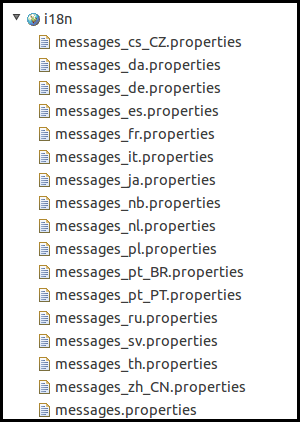
\includegraphics[width=4.3cm]{messages}
\caption{I18n (arquivos de propriedades).}
\label{I18nFig}
\end{figure}

As visões  geradas no  {\it scaffolding} de  nossa aplicação  estão parcialmente
internacionalizados. Ou seja,  pode-se observar que essas visões  incluem a {\it
  tag} {\bf  <g:message code>}, onde code é  uma referência a algum  termo a ser
internacionalizado.   O  nó  {\bf  i18n}  contém  um  conjunto  de  arquivos  de
propriedades   (termos   a  serem   traduzidos   para   diferentes  línguas)   –
Figura~\ref{I18nFig}.   É importante  salientar que  esses arquivos  são gerados
automaticamente  durante a execução  dos comandos  do Grails  ({\bf create-app},
{\bf create-controller}, {\bf generate-all}, etc).  

\begin{small}
\begin{cBox}
As   visões   são   os   locais   mais   comuns  para   o   uso   de   mensagens
internacionalizadas.  Para acessar  as  mensagens personalizadas  nas visões,  a
equipe de desenvolvimento basta utilizar a seguinte {\it tag} nas visões (*.gsp)
desenvolvidas: 

\vspace{0.2cm}

\verb#<g:message code="welcome.greeting" />#

\vspace{0.2cm}

\noindent Se  a equipe tiver  incluido uma chave no  arquivo messages.properties
(com  sufixo do {\it  Locale} apropriado),  tal como  ilustrada a  seguir, então
Grails apresenta a mensagem personalizada:

\vspace{0.2cm}

\verb#welcome.greeting = Good Morning. My name is Bob.#

\vspace{0.2cm}

\noindent Note  que em  algumas ocasiões é  necessário passar argumentos  para a
mensagem. Isso também é possível com a mesma {\it tag}:

\vspace{0.2cm}

\verb#<g:message code="welcome.greeting" args="${ ['Night','Bill'] }" />#

\vspace{0.2cm}

\noindent No entanto,  é necessário utilizar os parâmetros  de posicionamento na
mensagem.

\vspace{0.2cm}

\verb#welcome.greeting = Good {0}. My name is {1}.#
\end{cBox}
\end{small}

\noindent Note que o esforço  da equipe Web para internacionalizar sua aplicação
consiste em determinar  os termos a serem traduzidos, que  serão inseridos em um
arquivo  de  propriedades, e  depois  realizar  a  tradução para  as  diferentes
línguas.  As traduções serão armazenadas  em arquivos cujos nomes terminam com o
{\it Locale} (língua e região) desejado.

\vspace{0.2cm}

Figura~\ref{Agenda18nFig} apresenta algumas mensagens relacionadas às classes de
domínio  {\bf  Agencia}   que  foram  traduzidas  e  copiadas   para  o  arquivo
messages\_pt\_BR.properties   ({\it  Message   Bundle}  para   o   Português  do
Brasil).  Pode-se observar  que esse  arquivo contém  traduções para  o  nome da
classe assim como  para o nome de  cada um de seus atributos.  Além disso, foram
adicionadas  algumas mensagens  relacionadas à  página  de {\it  login} que  foi
gerada automaticamente pela execução do comando {\bf s2-quickstart}. 

\begin{figure}[htbp]
\begin{mdframed}
\begin{footnotesize}
\begin{verbatim}
# Agencia - mensagens
agencia.label = Agência
agencia.numero.label = Número
agencia.nome.label = Nome
agencia.endereco.label = Endereço
agencia.banco.label = Banco
agencia.gerentes.label = Gerentes

# Página de Login - mensagens
springSecurity.login.header = Login
springSecurity.login.remember.me.label = Lembre-me
springSecurity.login.button = Login
springSecurity.login.username.label = Login
springSecurity.login.password.label = Password
\end{verbatim}
\end{footnotesize}
\end{mdframed}
\caption{Messagens I18n para a classe de Domínio Usuario}
\label{Agenda18nFig}
\end{figure}

\begin{remark}
Um  bom exercício  consiste em  internacionalizar as  mensagens  relacionadas às
demais classes de domínio da aplicação {\bf ControleBancario}.  
\end{remark}

\section{Personalização dos templates utilizados no scaffolding}

Nessa seção  será apresentado o  processo de personalização dos  {\it templates}
utilizados pelo  mecanismo de {\it  scaffolding} na geração dos  controladores e
visões. No  contexto da aplicação {\bf  ControleBancario}, essas personalizações
tem  como   objetivo  gerar  os  controladores  e   visões  com  funcionalidades
relacionadas ao controle de acesso já incorporadas. Além disso, a personalização
é  realizada de  tal forma  que  as visões  {\bf create.gsp}  e {\bf  edit.gsp},
geradas pelo  {\it scaffolding},  já incorporam as  máscaras de entrada  para os
atributos CEP, CNPJ e CPF.

\vspace{0.2cm}

Portanto, o primeiro passo no  processo de personalização dos templates consiste
na execução do comando {\bf  install-templates}. Para tal, no IDE IntelliJ: abra
a  janela {\bf  Terminal} e  execute o  comando {\bf  grails install-templates}.
Esse comando copia os {\it templates} usadas nas atividades de geração de código
para o diretório {\bf src/main/templates/scaffolding}.  Esse diretório contém:
\index{Comandos!grails install-templates} 

\begin{itemize}

\vspace{0.2cm}

\item  Os  {\it templates}  utilizados  pelos  comandos \texttt{create-*}  ({\bf
  create-domain-class}, {\bf create-controller}, etc);

\vspace{0.2cm}

\item  Os {\it  templates} utilizados  pelos comandos  \texttt{generate-*} ({\bf
  generate-all},  {\bf  generate-controller},  {\bf generate-views},  etc).   No
  contexto desse tutorial, apenas  serão personalizados os {\it templates} dessa
  categoria; 

\end{itemize}

\newpage

\subsection{Template: Controller.groovy}

\vspace{0.5cm}

O  {\it plugin}  {\bf spring-security}  permite  a utilização  da anotação  {\bf
  @Secured} para aplicar regras de  controle de acesso aos controladores (e suas
respectivas  ações).   A  anotação  pode  ser  definida  a  nível  de  uma  ação
específica, que significa que os papéis especificados são necessários no acesso 
à aquela  ação ou a nível de  classe, que significa que  os papéis especificados
são     necessários      no     acesso      a     todas     as      ações     do
controlador. \index{Plugins!spring-security} 

\vspace{0.2cm}

O   {\it  template}  {\bf   Controller.groovy}  é   utilizado  na   geração  dos
controladores.   No  contexto da  aplicação  {\bf  ControleBancario}, esse  {\it
  template} será  alterado de tal  forma que o  acesso a ação {\bf  show()}, dos
controladores  da  aplicação, será  restrito  aos  usuários  que desempenham  os
respectivos papéis: {\bf ROLE\_ADMIN}, {\bf ROLE\_CLIENTE} e {\bf ROLE\_GERENTE}
(Código~\ref{codTemControl}, linha 14). As  demais ações dos controladores serão
restritas   ao  papel   {\bf  ROLE\_ADMIN}   (Código~\ref{codTemControl},  linha
7). Salienta-se que  esses papéis serão criados no  {\it Bootstrap} da aplicação
(Seção~\ref{secBootstrap2}).

\begin{lstlisting}[numbers=left, caption={\it Template} {\bf Controller.groovy},
    frame = trBL,float=htbp, label=codTemControl] 
<%=packageName ? "package ${packageName}" : ''%>

import static org.springframework.http.HttpStatus.*
import grails.transaction.Transactional
import org.springframework.security.access.annotation.Secured
@Transactional(readOnly = true)
@Secured ('ROLE_ADMIN')
class ${className}Controller {
    static allowedMethods = [save: "POST", update: "PUT", delete: "DELETE"]
    def index(Integer max) {
        params.max = Math.min(max ?: 10, 100)
        respond ${className}.list(params), model:[${propertyName}Count: ${className}.count()]
    }
    @Secured (['ROLE_ADMIN', 'ROLE_CLIENTE' , 'ROLE_GERENTE'])
    def show(${className} ${propertyName}) {
        respond ${propertyName}
    }
    def create() {
        respond new ${className}(params)
    }
    @Transactional
    def save(${className} ${propertyName}) {
        if (${propertyName} == null) {
            transactionStatus.setRollbackOnly()
            notFound()
            return
        }
        if (${propertyName}.hasErrors()) {
            transactionStatus.setRollbackOnly()
            respond ${propertyName}.errors, view:'create'
            return
        }
        ${propertyName}.save flush:true
        request.withFormat {
            form multipartForm {
            flash.message = message(code: 'default.created.message', args: [message(code: '${propertyName}.label', 
                                      default: '${className}'), ${propertyName}.id])
                redirect ${propertyName}
            }
            '*' { respond ${propertyName}, [status: CREATED] }
        }
    }
    def edit(${className} ${propertyName}) {
        respond ${propertyName}
    }
    @Transactional
    def update(${className} ${propertyName}) {
        if (${propertyName} == null) {
            transactionStatus.setRollbackOnly()
            notFound()
            return
        }
        if (${propertyName}.hasErrors()) {
            transactionStatus.setRollbackOnly()
            respond ${propertyName}.errors, view:'edit'
            return
        }
        ${propertyName}.save flush:true
        request.withFormat {
            form multipartForm {
            flash.message = message(code: 'default.updated.message', args: [message(code: '${propertyName}.label', 
                                    default: '${className}'), ${propertyName}.id])
                redirect ${propertyName}
            }
            '*'{ respond ${propertyName}, [status: OK] }
        }
    }
    @Transactional
    def delete(${className} ${propertyName}) {
        if (${propertyName} == null) {
            transactionStatus.setRollbackOnly()
            notFound()
            return
        }
        ${propertyName}.delete flush:true
        request.withFormat {
            form multipartForm {
            flash.message = message(code:'default.deleted.message', args: [message(code: '${propertyName}.label', 
                                    default: '${className}'), ${propertyName}.id])
                redirect action:"index", method:"GET"
            }
            '*'{ render status: NO_CONTENT }
        }
    }
    protected void notFound() {
        request.withFormat {
          form multipartForm {
          flash.message = message(code: 'default.not.found.message', args: [message(code: '${propertyName}.label', 
                                  default: '${className}'), params.id])
                redirect action: "index", method: "GET"
            }
            '*'{ render status: NOT_FOUND }
        }
    }
}
\end{lstlisting}

\subsection{Template: create.gsp}

\vspace{0.5cm}

O  {\it  template} {\bf  create.gsp}  é utilizado  na  geração  das visões  {\bf
  create()} associadas a cada um dos controladores da aplicação.  No contexto da
aplicação {\bf ControleBancario}, esse {\it template} será alterado de tal forma
que serão definidas máscaras de entrada (Código~\ref{codTemCreate}, linhas 7-16)
para os atributos CEP, CNPJ e CPF das classes de domínio.

\begin{figure}[htbp]
\centering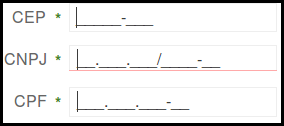
\includegraphics[width=8cm]{mascara}
\caption{Máscaras de entrada: CEP, CNPJ e CPF}
\label{figMascara}
\end{figure}

Figura~\ref{figMascara}  apresenta  um  exemplo  das  máscaras  de  entrada  dos
atributos  CEP, CNPJ  e CPF  da aplicação  {\bf ControleBancario}.  Na definição
dessas  máscaras de entrada,  foi utilizado  o {\it  plugin} {\bf  jQuery Masked
  Input}\footnote{\url{http://digitalbush.com/projects/masked-input-plugin/}}
que permite construir máscaras em campos HTML com as seguintes regras: 

\begin{itemize}

\vspace{0.3cm}

\item {\bf a} - Representa um caractere alfabético (A-Z, a-z)

\vspace{0.3cm}

\item {\bf 9} - Representa um digito (0-9)

\vspace{0.3cm}

\item {\bf *} - Representa um caractere alfanumérico (A-Z, a-z ,0-9)

\end{itemize}

\vspace{0.3cm}

Assim,  a máscara {\bf  999.999.999-99} define  um CPF  composto por  11 digitos
separados pelos caracteres: ponto ({\bf .}) e traço ({\bf -}).  

\vspace{0.3cm}

\begin{remark}
Análogo ao  {\bf create.gsp}, o  {\it template} {\bf edit.gsp}  também necessita
ser alterado para  definir as máscaras de entrada para os  atributos CEP, CNPJ e
CPF das classes  de domínio.  Então, fica como exercício  para o leitor realizar
tal alteração.
\end{remark}

\begin{lstlisting}[numbers=left, caption={\it  Template} {\bf create.gsp}, frame
    = trBL,float=htbp, label=codTemCreate]
<!DOCTYPE html>
<html>
    <head>
        <meta name="layout" content="main" />
        <g:set var="entityName" value="\${message(code: '${propertyName}.label', default: '${className}')}" />
        <title><g:message code="default.create.label" args="[entityName]" /></title>
        <asset:javascript src="jquery-2.2.0.min.js" />
        <asset:javascript src="jquery.maskedinput.min.js" />
        <g:javascript>
            var JQuery = jQuery.noConflict()
            JQuery(document).ready(function(){
                JQuery("#CPF").mask("999.999.999-99");
                JQuery("#CNPJ").mask("99.999.999/9999-99");
                JQuery("#CEP").mask("99999-999");
            });
        </g:javascript>
    </head>
    <body>
        <a href="#create-${propertyName}" class="skip" tabindex="-1"><g:message code="default.link.skip.label" 
                                                                      default="Skip to content&hellip;"/></a>
        <div class="nav" role="navigation">
            <ul>
                <li><a class="home" href="\${createLink(uri: '/')}"><g:message code="default.home.label"/></a></li>
                <li><g:link class="list" action="index">
                      <g:message code="default.list.label" args="[entityName]" />
                    </g:link></li>
            </ul>
        </div>
        <div id="create-${propertyName}" class="content scaffold-create" role="main">
            <h1><g:message code="default.create.label" args="[entityName]" /></h1>
            <g:if test="\${flash.message}">
            <div class="message" role="status">\${flash.message}</div>
            </g:if>
            <g:hasErrors bean="\${this.${propertyName}}">
            <ul class="errors" role="alert">
                <g:eachError bean="\${this.${propertyName}}" var="error">
                <li <g:if test="\${error in org.springframework.validation.FieldError}">
                data-field-id="\${error.field}" </g:if>><g:message error="\${error}"/></li>
                </g:eachError>
            </ul>
            </g:hasErrors>
            <g:form action="save">
                <fieldset class="form">
                    <f:all bean="${propertyName}"/>
                </fieldset>
                <fieldset class="buttons">
                    <g:submitButton name="create" class="save" 
                    value="\${message(code: 'default.button.create.label', default: 'Create')}" />
                </fieldset>
            </g:form>
        </div>
    </body>
</html> 
\end{lstlisting}

\subsection{Template: index.gsp}

\vspace{0.5cm}

O {\it template}  {\bf index.gsp} é utilizado na geração  das visões {\bf index}
associadas a cada  um dos controladores da aplicação.   No contexto da aplicação
{\bf     ControleBancario},     esse     {\it    template}     será     alterado
(Código~\ref{codTemIndex}, linhas  14-16) de tal forma  que o {\it  link} para a
operação de criação  de entidades (ação {\bf create()})  apenas será apresentada
se o  usuário encontra-se  autenticado e possui  papel necessário  para executar
essa ação. 

\begin{lstlisting}[numbers=left, caption={\it Template} {\bf index.gsp}, frame =
    trBL,float=htbp, label=codTemIndex] 
<!DOCTYPE html>
<html>
    <head>
        <meta name="layout" content="main" />
        <g:set var="entityName" value="\${message(code: '${propertyName}.label', default: '${className}')}" />
        <title><g:message code="default.list.label" args="[entityName]" /></title>
    </head>
    <body>
        <a href="#list-${propertyName}" class="skip" tabindex="-1"><g:message code="default.link.skip.label" 
                                                                   default="Skip to content&hellip;"/></a>
        <div class="nav" role="navigation">
            <ul>
                <li><a class="home" href="\${createLink(uri: '/')}"><g:message code="default.home.label"/></a></li>
                <sec:access controller="${propertyName}" action='create'>
                    <li><g:link class="create" action="create"><g:message code="default.new.label" 
                                                               args="[entityName]" /></g:link></li>
                </sec:access>
            </ul>
        </div>
        <div id="list-${propertyName}" class="content scaffold-list" role="main">
            <h1><g:message code="default.list.label" args="[entityName]" /></h1>
            <g:if test="\${flash.message}">
                <div class="message" role="status">\${flash.message}</div>
            </g:if>
            <f:table collection="\${${propertyName}List}" />

            <div class="pagination">
                <g:paginate total="\${${propertyName}Count ?: 0}" />
            </div>
        </div>
    </body>
</html>
\end{lstlisting}

O {\it plugin} {\bf spring-security} define algumas {\it tags} GSP que permite a
exibição  condicional de {\it  links} de  acesso a  ações de  controladores.  Ou
seja,  aquele {\it  link} apenas  será  apresentado em  uma visão  se o  usuário
encontra-se autenticado e possui papel necessário para executar a ação.
\index{Plugins!spring-security} 

\vspace{0.2cm}

Por exemplo, a {\it tag}  GSP {\bf <sec: ifLoggedin>} apresentada abaixo, apenas
renderizaria a mensagem {\em Bemvindo!}, se o usuário encontra-se autenticado.

\vspace{0.3cm}

\begin{cBox}
\begin{footnotesize}
\begin{verbatim}
<sec:ifLoggedIn>
Bemvindo!
</sec:ifLoggedIn>
\end{verbatim}
\end{footnotesize}
\end{cBox}

\vspace{0.3cm}

Como  outro  exemplo,  a  {\it  tag}  GSP {\bf  <sec:  access>}  abaixo,  apenas
renderizaria  o  {\it  link}  para  a  ação {\bf  create}  do  controlador  {\bf
  transacao},  se o usuário  encontra-se autenticado  e possui  papel necessário
para executar a ação.  

\vspace{0.3cm}

\begin{cBox}
\begin{footnotesize}
\begin{verbatim}
<sec:access controller='transacao' action='create'>
   <g:link controller='transacao' action='create'>Cria Transação</g:link>
</sec:access>
\end{verbatim}
\end{footnotesize}
\end{cBox}

\vspace{0.3cm}

Para maiores  informações sobre as {\it  tags} GSP, definidas  pelo {\it plugin}
{\bf   spring-security},  o   leitor   pode  consultar   o  seguinte   endereço:
\url{http://grails.org/plugin/spring-security-core}. 

\subsection{Template: show.gsp}

\vspace{0.5cm}

O {\it  template} {\bf show.gsp}  é utilizado na  geração das visões  {\bf show}
associadas a cada  um dos controladores da aplicação.   No contexto da aplicação
{\bf  ControleBancario}, esse  {\it  template} será  alterado  para refletir  as
seguintes funcionalidades:

\vspace{0.3cm}

\begin{itemize}

\item O {\it  link} para a operação de criação de  entidades (ação {\bf create})
  apenas será  apresentada se o  usuário encontra-se autenticado e  possui papel
  necessário para executar essa ação (Código~\ref{codTemShow}, linhas 16-19). 

\vspace{0.3cm}

\item  O botão {\bf  edit}, responsável  pela edição  de entidades,  apenas será
  apresentada  se o usuário  encontra-se autenticado  e possui  papel necessário
  para executar essa ação (Código~\ref{codTemShow}, linhas 30-33).  

\vspace{0.3cm}
 
\item O botão  {\bf delete}, responsável pela remoção  de entidades, apenas será
  apresentada  se o usuário  encontra-se autenticado  e possui  papel necessário
  para executar essa ação (Código~\ref{codTemShow}, linhas 34-38).

\end{itemize}

\begin{lstlisting}[numbers=left, caption={\it Template}  {\bf show.gsp}, frame =
    trBL,float=htbp, label=codTemShow] 
<!DOCTYPE html>
<html>
    <head>
        <meta name="layout" content="main" />
        <g:set var="entityName" value="\${message(code: '${propertyName}.label', default: '${className}')}" />
        <title><g:message code="default.show.label" args="[entityName]" /></title>
    </head>
    <body>
        <a href="#show-${propertyName}" class="skip" tabindex="-1"><g:message code="default.link.skip.label" 
                                        default="Skip to content&hellip;"/></a>
        <div class="nav" role="navigation">
            <ul>
                <li><a class="home" href="\${createLink(uri: '/')}"><g:message code="default.home.label"/></a></li>
                <li><g:link class="list" action="index"><g:message code="default.list.label" 
                                         args="[entityName]" /></g:link></li>
                <sec:access controller="${propertyName}" action='create'>
                    <li><g:link class="create" action="create"><g:message code="default.new.label" 
                                                                args="[entityName]" /></g:link></li>
                </sec:access>
            </ul>
        </div>
        <div id="show-${propertyName}" class="content scaffold-show" role="main">
            <h1><g:message code="default.show.label" args="[entityName]" /></h1>
            <g:if test="\${flash.message}">
            <div class="message" role="status">\${flash.message}</div>
            </g:if>
            <f:display bean="${propertyName}" />
            <g:form resource="\${this.${propertyName}}" method="DELETE">
                <fieldset class="buttons">
                    <sec:access controller="${propertyName}" action='edit'>
                        <g:link class="edit" action="edit" resource="\${this.${propertyName}}">
                            <g:message code="default.button.edit.label" default="Edit" /></g:link>
                    </sec:access>
                    <sec:access controller="${propertyName}" action='delete'>
                        <input class="delete" type="submit" value="\${message(code: 'default.button.delete.label', 
                                      default: 'Delete')}" onclick="return confirm('\${message(code: 
                                      'default.button.delete.confirm.message', default: 'Are you sure?')}');" />
                    </sec:access>
                </fieldset>
            </g:form>
        </div>
    </body>
</html>
\end{lstlisting}

\newpage

\section{Controladores e Visões}

\hyphenation{Terminal}

Após realizar as alterações discutidas  na seção anterior, é necessário executar
o  comando  {\bf generate-all}  para  que  as  alterações nos  {\it  templates},
discutidos na  seção anterior,  sejam refletidos nos  controladores e  visões da
aplicação {\bf ControleBancario}.  No IDE IntelliJ: abra a janela {\bf Terminal}
e execute o comando {\bf grails generate-all br.ufscar.dc.dsw.Agencia}. Repita a
execução   desse   comando   para    as   classes   de   domínio   listadas   na
Tabela~\ref{tblGenerateAll}.
\index{Comandos!grails generate-all} 

\begin{table}[htbp]
\centering
\begin{tabular}{|c|c|c|c|c|}
\hline
\rowcolor{Gray}
Agencia & Banco & CaixaEletronico & Cidade & ClienteFisico \\ \hline
\rowcolor{C2}
ClienteJuridico & ContaCliente & ContaCorrente & ContaPoupanca & Endereco \\ \hline
\rowcolor{Gray}
Estado & Gerente &Transacao & &\\ \hline
\end{tabular}
\caption{Classes de domínio: geração dos Controladores e Visões.}
\label{tblGenerateAll}
\end{table}

\subsection{Controlador: ContaController}

\vspace{0.5cm}

O  próximo passo  consiste na  definição  do {\bf  ContaController} associado  à
classe  de  domínio {\bf  Conta}.   Esse  controlador  implementa operações  que
uniformiza o acesso às instâncias das subclasses da classe abstrata {\bf Conta}.
Por exemplo, a ação {\bf index()} é responsável por listar contas bancárias (não
importando se elas são contas correntes ou contas poupanças).

\vspace{0.2cm}

Para criar um  controlador, relacionado à classe de domínio  {\bf Conta}, no IDE
IntelliJ:  abra  a  janela  {\bf  Terminal}  e execute  o  comando  {\bf  grails
  create-controller   br.ufscar.dc.dsw.Conta}.     Abra   o   controlador   {\bf
  ContaController}      e     implemente-o      conforme      apresentado     no
Código~\ref{codContaController}.  
\index{Comandos!grails create-controller}

\begin{lstlisting}[caption=Controlador    {\bf    ContaController},   frame    =
    trBL,float=htbp, label=codContaController] 
package br.ufscar.dc.dsw

import static org.springframework.http.HttpStatus.*
import grails.transaction.Transactional
import org.springframework.security.access.annotation.Secured

@Secured('ROLE_GERENTE')
class ContaController {
    
    static allowedMethods = [save: "POST", update: "PUT", delete: "DELETE"]
    
    def index(Integer max) {
        params.max = Math.min(max ?: 10, 100)
        respond Conta.list(params), model:[list: Conta.list(params), contaCount: Conta.count()]
    }
    
    @Secured(['ROLE_ADMIN', 'ROLE_CLIENTE', 'ROLE_GERENTE'])
    def show() {
        Conta instance = Conta.get(params.id)
        if (instance.instanceOf(ContaCorrente)) {
            forward controller: 'contaCorrente', action: "show"
        } else {
            forward controller: 'contaPoupanca', action: "show"
        }
    }
}

\end{lstlisting}

\begin{itemize}

\item A ação {\bf index()} é  restrita aos usuários que desempenham o papel {\bf
  ROLE\_GERENTE}; e 

\vspace{0,3cm}

\item A  ação {\bf show()}  é restrita aos  usuários que desempenham  os papéis:
  {\bf ROLE\_ADMIN}, {\bf ROLE\_CLIENTE} e {\bf ROLE\_GERENTE}. Além disso, essa
  ação  verifica  se a  instância  é  uma conta  corrente  ou  conta poupança  e
  direciona para o controlador mais apropriado: {\bf ContaCorrenteController} ou
  {\bf ContaPoupancaController}.  

\end{itemize}

\subsection{Visão: conta/index.gsp}

\vspace{0.5cm}

Relembrando   a   discussão  da   Seção~\ref{secEstatico},   para  cada   método
correspondente a  uma ação em um  controlador é criada  uma correspondente visão
(arquivo  com  extensão  {\bf  .gsp}).  Assim,  a  ação  {\bf  index},  de  {\bf
  ContaController}, tem o correspondente {\bf index.gsp}.  

\vspace{0.2cm}

A visão {\bf index.gsp} apresenta  uma lista de contas bancárias (não importando
se elas são  contas correntes ou contas poupanças).  A implementação dessa visão
encontra-se apresentada no Código~\ref{codContaIndex}. 

\vspace{0.3cm}

\begin{lstlisting}[caption=Visão  {\bf  conta/index.gsp}, frame=trBL,float=htbp,
    label=codContaIndex] 
<%@ page import="br.ufscar.dc.dsw.Conta" %>
<!DOCTYPE html>
<html>
	<head>
		<meta name="layout" content="main">
		<g:set var="entityName" value="${message(code: 'conta.label', default: 'Conta')}" />
		<title><g:message code="default.list.label" args="[entityName]" /></title>
	</head>
	<body>
		<a href="#list-conta" class="skip" tabindex="-1"><g:message code="default.link.skip.label" 
                                                                  default="Skip to content&hellip;"/></a>
		<div class="nav" role="navigation">
			<ul>
				<li><a class="home" href="${createLink(uri: '/')}"><g:message code="default.home.label"/></a></li>
			</ul>
		</div>
		<div id="list-conta" class="content scaffold-list" role="main">
			<h1><g:message code="default.list.label" args="[entityName]" /></h1>
			<g:if test="${flash.message}">
				<div class="message" role="status">${flash.message}</div>
			</g:if>
			<table>
			<thead>
				<tr>
					<g:sortableColumn property="numero" title="${message(code: 'conta.numero.label', default: 'Numero')}" />
					<th><g:message code="conta.agencia.label" default="Agencia" /></th>
					<g:sortableColumn property="saldo" title="${message(code: 'conta.saldo.label', default: 'Saldo')}" />
					<g:sortableColumn property="abertura" title="${message(code: 'conta.abertura.label', 
                                                                                     default: 'Abertura')}" />
				</tr>
			</thead>
				<tbody>
				<g:each in="${list}" status="i" var="conta">
					<tr class="${(i % 2) == 0 ? 'even' : 'odd'}">
						<td><g:link action="show" controller="${conta.class}" id="${conta.id}">
                                                ${fieldValue(bean: conta, field: "numero")}</g:link></td>
						<td>${fieldValue(bean: conta, field: "agencia")}</td>
						<td>${fieldValue(bean: conta, field: "saldo")}</td>
						<td><g:formatDate date="${conta.abertura}" /></td>
					</tr>
				</g:each>
				</tbody>
			</table>
			<div class="pagination">
				<g:paginate total="${contaCount ?: 0}" />
			</div>
		</div>
	</body>
</html>
\end{lstlisting}

\vspace{0.3cm}

\noindent Conforme pode-se observar, essa  visão constrói uma tabela HTML com os
atributos  (número, agência,  saldo e  data  de abertura)  das contas  bancárias
retornadas.   É importante  salientar  que  é através  da  variável {\bf  list},
retornada pela  ação {\bf index()},  que essa visão  tem acesso aos  valores dos
atributos das contas bancárias.  

\newpage

\subsection{Controlador: ClienteController}

\vspace{0.5cm}

Análogo ao {\bf ContaControlador}, o {\bf ClienteController}, associado à classe
de  domínio {\bf  Cliente},  implementa  operações que  uniformiza  o acesso  às
instâncias das subclasses da classe abstrata {\bf Cliente}.  Por exemplo, a ação
{\bf  index()} é responsável  por listar  clientes (não  importando se  eles são
clientes físicos ou jurídicos). 

\vspace{0.3cm}

Para criar um  controlador, relacionado à classe de domínio  {\bf Conta}, no IDE
IntelliJ:  abra  a  janela  {\bf  Terminal}  e execute  o  comando  {\bf  grails
  create-controller   br.ufscar.dc.dsw.Cliente}.    Abra   o  controlador   {\bf
  ClienteController}     e      implemente-o     conforme     apresentado     no
Código~\ref{codClienteController}.  
\index{Comandos!grails create-controller}

\begin{lstlisting}[caption=Controlador          {\bf         ClienteController},
    frame=trBL,float=htbp, label=codClienteController] 
package br.ufscar.dc.dsw

import static org.springframework.http.HttpStatus.*
import grails.transaction.Transactional
import org.springframework.security.access.annotation.Secured

@Secured('ROLE_GERENTE')
class ClienteController {
    
    static allowedMethods = [save: "POST", update: "PUT", delete: "DELETE"]
    def index(Integer max) {
        params.max = Math.min(max ?: 10, 100)
        respond Cliente.list(params), model:[list: Cliente.list(params), clienteCount: Cliente.count()]
    }
    
    @Secured(['ROLE_ADMIN', 'ROLE_CLIENTE', 'ROLE_GERENTE'])
    def show() {
        Cliente instance = Cliente.get(params.id)
        if (instance.instanceOf(ClienteFisico)) {
            forward controller: 'clienteFisico', action: "show"
        } else {
            forward controller: 'clienteJuridico', action: "show"
        }
    }
}
\end{lstlisting}

\begin{itemize}

\item A ação {\bf index()} é  restrita aos usuários que desempenham o papel {\bf
  ROLE\_GERENTE}; e 

\vspace{0,3cm}

\item A ação {\bf show()} é restrita aos usuários que desempenham os respectivos
  papéis:  {\bf ROLE\_ADMIN},  {\bf ROLE\_CLIENTE}  e {\bf  ROLE\_GERENTE}. Além
  disso,  essa ação  verifica se  a  instância é  um cliente  físico ou  cliente
  jurídico   e   direciona   para    o   controlador   mais   apropriado:   {\bf
    ClienteFisicoController} ou {\bf ClienteJuridicoController}.  

\end{itemize}

\vspace{0.3cm}

\subsection{Visão: cliente/index.gsp}

\vspace{0.5cm}

A visão {\bf index.gsp} apresenta uma  lista de clientes (não importando se eles
são  clientes físicos ou  jurídicos).  A  implementação dessa  visão encontra-se
apresentada no Código~\ref{codCliIndex}. 

\vspace{0.3cm}

\begin{itemize}

\item  Conforme pode-se observar,  essa visão  constrói uma  tabela HTML  com os
  atributos (nome, endereço, data de  moradia e status) dos clientes retornados.
  É importante  salientar que é através  da variável {\bf  list}, retornada pela
  ação {\bf  index()}, que essa visão  tem acesso aos valores  dos atributos dos
  clientes.  

\end{itemize}

\newpage

\begin{lstlisting}[caption=Visão       {\bf       cliente/index.gsp},      frame
    =trBL,float=htbp, label=codCliIndex] 
<%@ page import="br.ufscar.dc.dsw.Cliente" %>
<!DOCTYPE html>
<html>
	<head>
		<meta name="layout" content="main">
		<g:set var="entityName" value="${message(code: 'cliente.label', default: 'Cliente')}" />
		<title><g:message code="default.list.label" args="[entityName]" /></title>
	</head>
	<body>
		<a href="#list-cliente" class="skip" tabindex="-1"><g:message code="default.link.skip.label" default="Skip to content&hellip;"/></a>
		<div class="nav" role="navigation">
			<ul>
				<li><a class="home" href="${createLink(uri: '/')}"><g:message code="default.home.label"/></a></li>
			</ul>
		</div>
		<div id="list-cliente" class="content scaffold-list" role="main">
			<h1><g:message code="default.list.label" args="[entityName]" /></h1>
			<g:if test="${flash.message}">
				<div class="message" role="status">${flash.message}</div>
			</g:if>
			<table>
			<thead>
					<tr>
						<g:sortableColumn property="nome" title="${message(code: 'cliente.nome.label', default: 'Nome')}" />
						<th><g:message code="cliente.endereco.label" default="Endereco" /></th>
						<g:sortableColumn property="dtMoradia" title="${message(code: 'cliente.dtMoradia.label', default: 'Dt Moradia')}" />
						<g:sortableColumn property="status" title="${message(code: 'cliente.status.label', default: 'Status')}" />
					</tr>
				</thead>
				<tbody>
				<g:each in="${list}" status="i" var="cliente">
					<tr class="${(i % 2) == 0 ? 'even' : 'odd'}">
						<td><g:link action="show" controller="${cliente.class}" id="${cliente.id}">${fieldValue(bean: cliente, field: "nome")}</g:link></td>
						<td>${fieldValue(bean: cliente, field: "endereco")}</td>
						<td><g:formatDate date="${cliente.dtMoradia}" /></td>
						<td>${fieldValue(bean: cliente, field: "status")}</td>
					</tr>
				</g:each>
				</tbody>
			</table>
			<div class="pagination">
				<g:paginate total="${clienteCount ?: 0}" />
			</div>
		</div>
	</body>
</html>
\end{lstlisting}

\subsection{Mapeamento URL}\index{URL!Mapeamento}

\vspace{0.3cm}

\hyphenation{MainController}

Pela convenção, ao executar a aplicação,  a página principal é a que lista todos
os  controladores da  aplicação.  Porém  é possível  alterar o  controlador {\bf
  URLMappings}                  --                  arquivo                 {\bf
  grails-app/controllers/controlebancario/URLMapping.groovy}  para definir outro
controlador/ação  padrão.   Código~\ref{codURLMappings}  define, como  a  página
principal,   a  ação   {\bf   index()}  do   controlador  {\bf   MainController}
(Seção~\ref{secMainController}).

\begin{lstlisting}[caption={\bf   URLMappings.groovy},  frame=trBL,  float=htbp,
    label=codURLMappings] 
class UrlMappings {
	static mappings = {
        "/$controller/$action?/$id?(.$format)?"{
            constraints {
                // apply constraints here
            }
        }
        "/"(controller:"main")
        "500"(view:'/error')
	}
}
\end{lstlisting}

\newpage

\subsection{Controlador: MainController}\label{secMainController}

\hyphenation{MainController}

\vspace{0.5cm}

O  {\bf MainController}  consiste  no controlador  principal  da aplicação  {\bf
  ControleBancario}.   Para  criar o  controlador  {\bf  MainController} no  IDE
IntelliJ:  abra  a  janela  {\bf  Terminal}  e execute  o  comando  {\bf  grails
  create-controller  br.ufscar.dc.dsw.MainController}.  Abra o  controlador {\bf
  MainController}      e      implemente-o      conforme     apresentado      no
Código~\ref{codMainController}.  
\index{Comandos!grails create-controller}

\begin{lstlisting}[caption=Controlador    {\bf    MainController},   frame=trBL,
    float=htbp, label=codMainController] 
package br.ufscar.dc.dsw

import org.springframework.security.access.annotation.Secured

@Secured(['ROLE_ADMIN', 'ROLE_CLIENTE', 'ROLE_GERENTE'])
class MainController {

    def index() { }
}
\end{lstlisting}

\begin{itemize}

\item  A  ação  {\bf  index()}  é  restrita  aos  usuários  que  desempenham  os
  respectivos   papéis:   {\bf   ROLE\_ADMIN},   {\bf  ROLE\_CLIENTE}   e   {\bf
    ROLE\_GERENTE}.  

\end{itemize}

\subsection{Visão: main/index.gsp}

\vspace{0.5cm}

A  visão {\bf  main/index.gsp} consiste  na  visão principal  da aplicação  {\bf
  ControleBancario}.   A implementação  dessa visão  encontra-se  apresentada no
Código~\ref{codMainIndex}.  

\lstset{language=XML}
\begin{lstlisting}[numbers=left, caption=Visão {\bf main/index.gsp}, frame=trBL,
    float=htbp, label=codMainIndex] 
<!DOCTYPE html>
<html>
 <head>
  <meta name="layout" content="main">
  <g:javascript library="jquery" />
 </head>
 <body>
  <div id="status" role="complementary">
   <h1>Op^çõ^es</h1>
   <table>
    <g:each var="c" in="${grailsApplication.controllerClasses.sort { it.fullName } }">
     <g:set var="name" value="${c.logicalPropertyName}" />
     <g:if test="${name != 'logout' && name != 'login' && name != 'main'}">
      <sec:access url='${createLink(controller: c.logicalPropertyName, base: "/")}'>
       <tr><td>    
        <g:link controller="${c.logicalPropertyName}">${c.naturalName.replace(" Controller","")}</g:link>
       </td></tr>
      </sec:access>
     </g:if>
    </g:each>
   </table>
  </div>
 </body>
</html>
\end{lstlisting}

Pode-se  observar,  pelas  linhas  14-18,   que  a  visão  apenas  apresenta  os
controladores para qual o usuário autenticado tem permissão de acessá-lo. Assim,
para  os usuários  que  desempenham  diferentes papéis,  a  página principal  da
aplicação {\bf ControleBancario} torna-se diferente. 

\vspace{0.2cm}

Figura~\ref{figVisao}(a) apresenta  a página principal conforme  acessada por um
usuário    que     desempenha    o    papel     {\bf    ROLE\_ADMIN}    enquanto
Figura~\ref{figVisao}(b)  apresenta  a página  principal  conforme acessada  por
usuário que desempenha o papel {\bf ROLE\_GERENTE}.  

\newpage

\begin{figure}[htbp]
\center
\subfigure[Visão: Papel Administrador]{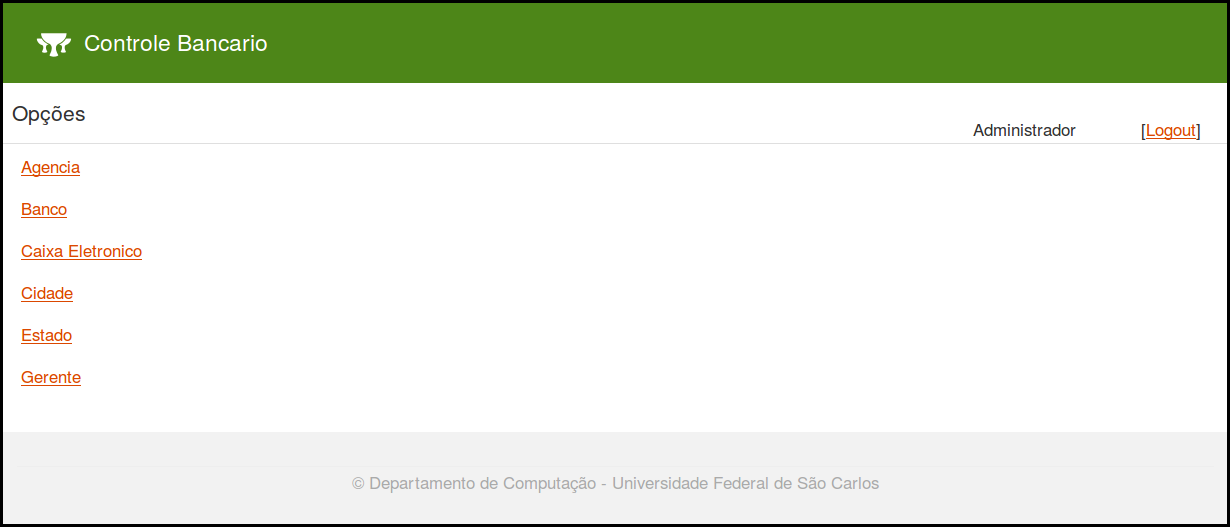
\includegraphics[width=7cm]{VisaoAdmin}}
\qquad
\subfigure[Visão: Papel Gerente]{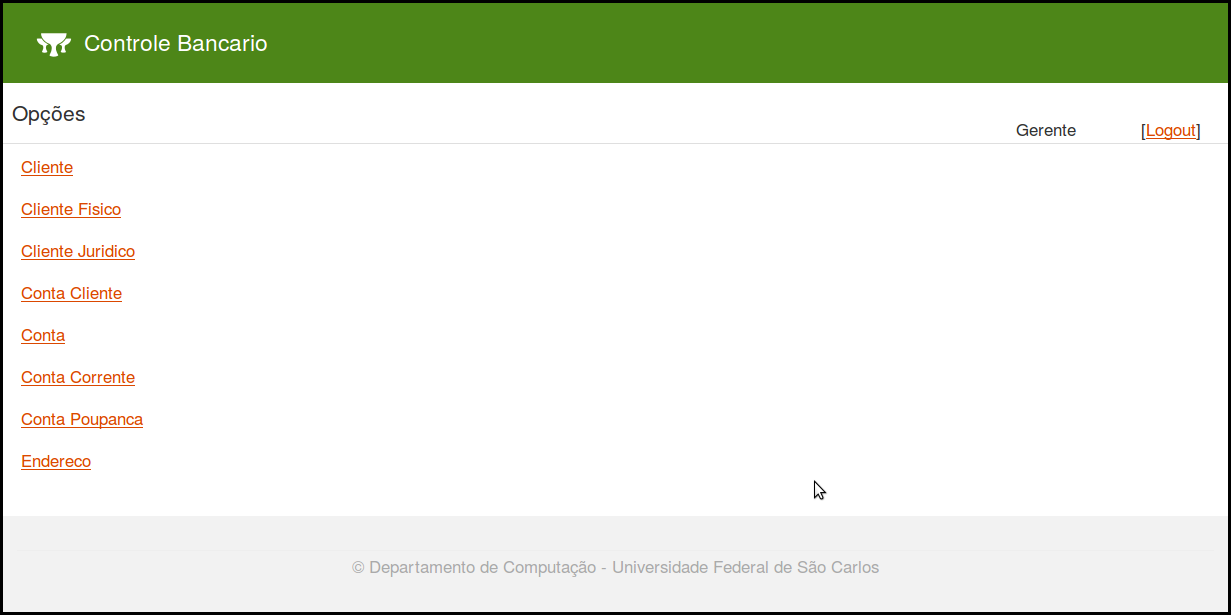
\includegraphics[width=6.5cm]{VisaoGerente}}
\caption{Visão main/index.gsp: diferentes visões}
\label{figVisao}
\end{figure}

\subsection{Controladores: últimas alterações relacionadas ao controle de acesso}

\vspace{0.3cm}

Por  fim, atualize os  controladores conforme  o Código~\ref{codControleAcesso}.
Pelo código, observa-se que: 

\vspace{0.3cm}

\begin{itemize}

\hyphenation{ContaClienteController}

\item      Os     controladores     {\bf      ClienteFisicoController},     {\bf
  ClienteJuridicoController},       {\bf      ContaClienteController},      {\bf
  ContaCorrenteController},     {\bf     ContaPoupancaController}     e     {\bf
  EnderecoController}  serão apenas  acessados  por usuários  que desempenham  o
  papel de gerente; e 

\vspace{0.3cm}

\item O controlador {\bf  TransacaoController} será apenas acessado por usuários
  que desempenham o papel de cliente.

\end{itemize}

\begin{lstlisting}[caption=Controladores  - últimas  alterações  relacionadas ao
    Controle de Acesso, frame = trBL,float=htbp, label=codControleAcesso] 
@Secured('ROLE_GERENTE')
class ClienteFisicoController {
  // Implementa^çã^o do controlador ClienteFisico
}

@Secured('ROLE_GERENTE')
class ClienteJuridicoController {
  // Implementa^çã^o do controlador ClienteJuridico
}

@Secured('ROLE_GERENTE')
class ContaClienteController {
  // Implementa^çã^o do controlador ClienteCliente
}

@Secured('ROLE_GERENTE')
class ContaCorrenteController {
  // Implementa^çã^o do controlador ContaCorrente
}

@Secured('ROLE_GERENTE')
class ContaPoupancaController {
  // Implementa^çã^o do controlador ContaPoupanca
}

@Secured('ROLE_GERENTE')
class EnderecoController {
  // Implementa^çã^o do controlador Endereco
}

@Secured('ROLE_CLIENTE')
class TransacaoController {
  // Implementa^çã^o do controlador Transacao
}
\end{lstlisting}

\newpage

\section{Melhorando o leiaute da aplicação: biblioteca de marca}

\vspace{0.3cm}

Com  o objetivo  de melhorar  o  leiaute da  aplicação, essa  seção apresenta  a
implementação de uma biblioteca de marca ({\it taglib}) que é utilizada em todas
as visões da aplicação {\bf ControleBancario}. Os passos são descritos a seguir: 

\begin{itemize}

\vspace{0.3cm}

\item Para  criar uma biblioteca  de marca, no  IDE GGTS: Selecione  {\bf Grails
  Tools} $\Longrightarrow$ {\bf Create TagLib}.   Digite {\bf Login} como o nome
  da biblioteca de  marca e clique em {\bf Finish}. Abra  a biblioteca de marcas
  {\bf     LoginTagLib}    e     implemente-o     conforme    apresentado     no
  Código~\ref{codTagLib}.  Pelo código-fonte, observa-se que essa classe imprime
  o nome do papel desempenhado pelo usuário {\it logado}.  

\begin{lstlisting}[caption=Biblioteca  de marca  {\bf  LoginTagLib}, frame=trBL,
    float=htbp, label=codTagLib] 
class LoginTagLib {
    def springSecurityService
    def loginControl = {
        if (springSecurityService.isLoggedIn()) {
            def usuario = springSecurityService.getCurrentUser()
            def authority = usuario.getAuthorities()[0].getAuthority()
            def papel
            if (authority.equals('ROLE_ADMIN')) {
                papel = "Administrador"
            } else if (authority.equals('ROLE_CLIENTE')) {
                papel = "Cliente"
            } else {
                papel = "Gerente"
            }
            out << "<span style=\"padding-right:50px\">" << papel << "</span>"
            out << "<span style=\"padding-right:25px\">"
            out << """ [${link(controller: "logout"){"Logout"}}]"""
            out << "</span>"
        }
    }
}
\end{lstlisting}

\item Inclua o  {\it template} \_footer (grails-app/views/layouts/\_footer.gsp)
  com o  conteúdo apresentado  na Listagem~\ref{footerLst}. Esse  {\it template}
  será o rodapé presente em todas as visões da aplicação.

\lstset{language=XML}
\begin{lstlisting}[caption={\it   Template}   {\bf  \_footer.gsp},   frame=trBL,
    float=htbp, label=footerLst] 
<div id="footer">
 <hr/> &copy; DC - UFSCar
</div>
\end{lstlisting}

\item Incluir o  {\it template} \_header (grails-app/views/layouts/\_header.gsp)
  com o  conteúdo apresentado  na Listagem~\ref{headerLst}. Esse  {\it template}
  será o cabeçalho presente em todas as visões da aplicação. Observa-se que esse
  {\it  template} utiliza  a  biblioteca de  marcas  {\bf LoginTagLib}  definida
  anteriormente. 

\lstset{language=XML}
\begin{lstlisting}[caption={\it   Template}   {\bf  \_header.gsp},   frame=trBL,
    float=htbp, label=headerLst]
<div id="header">
    <div id = "loginHeader">
        </br>
        <g:loginControl/>
    </div>
</div>
\end{lstlisting}

\newpage

\item    No     leaiute    padrão,    utilizado    por     todas    as    visões
  (arquivo  grails-app/views/layouts/main.gsp), realize  as  alterações conforme
  apresentadas pelo Código~\ref{codMain}.  Pelo código-fonte, observa-se que:

\begin{itemize}

\vspace{0.3cm}

\item O nome da aplicação ({\bf ControleBancario}) é inserido (linha 29);

\vspace{0.3cm}

\item O {\it template} {\bf  header}, definido anteriormente, é utilizado (linha
  40); e 

\vspace{0.3cm}

\item O {\it template} {\bf  footer}, definido anteriormente, é utilizado (linha
  42). 

\end{itemize}

\lstset{language=XML}
\begin{lstlisting}[numbers=left,        caption=Leiaute        padrão       {\bf
      grails-app/views/layouts/main.gsp}, frame=trBL,float=htbp, label=codMain] 
<!doctype html>
<html lang="en" class="no-js">
<head>
    <meta http-equiv="Content-Type" content="text/html; charset=UTF-8"/>
    <meta http-equiv="X-UA-Compatible" content="IE=edge"/>
    <title>
        <g:layoutTitle default="Grails"/>
    </title>
    <meta name="viewport" content="width=device-width, initial-scale=1"/>
    <asset:stylesheet src="application.css"/>
    <g:layoutHead/>
</head>
<body>
    <div class="navbar navbar-default navbar-static-top" role="navigation">
        <div class="container">
            <div class="navbar-header">
                <button type="button" class="navbar-toggle" data-toggle="collapse" data-target=".navbar-collapse">
                    <span class="sr-only">Toggle navigation</span>
                    <span class="icon-bar"></span>
                    <span class="icon-bar"></span>
                    <span class="icon-bar"></span>
                </button>
                <a class="navbar-brand" href="/#">
                    <i class="fa grails-icon">
                        <asset:image src="grails-cupsonly-logo-white.svg"/>
                    </i>Controle Bancario
                </a>
            </div>
            <div class="navbar-collapse collapse" aria-expanded="false" style="height: 0.8px;">
                <ul class="nav navbar-nav navbar-right">
                    <g:pageProperty name="page.nav" />
                </ul>
            </div>
        </div>
    </div>
    <g:render template="/layouts/header" />
    <g:layoutBody/>
    <g:render template="/layouts/footer" />
    <div class="footer" role="contentinfo"></div>
    <div id="spinner" class="spinner" style="display:none;">
        <g:message code="spinner.alt" default="Loading&hellip;"/>
    </div>
    <asset:javascript src="application.js"/>
</body>
</html>
\end{lstlisting}

\item     Por     fim,     adicione     as    linhas     no     arquivo     {\bf
  grails-app/assets/stylesheets/main.css}      conforme      apresentado      no
  Código~\ref{mainCSSLst}.  

\lstset{language=XML}
\begin{lstlisting}[caption=Arquivo   {\bf  main.css},   frame=trBL,  float=htbp,
    label=mainCSSLst] 
#footer {
    font-size: 0.75em;
    font-style: italic;
    padding: 2em 1em 2em 1em;
    margin-bottom: 1em;
    margin-top: 1em;
    clear: both;
}

#loginHeader {
    float: right;
}
\end{lstlisting}

\end{itemize}

\section{Executando a aplicação}\label{secBootstrap2}

\vspace{0.3cm}

Conforme discutido anteriormente, antes  de executar a aplicação, instâncias das
entidades serão criadas.  No caso,  serão criados instâncias das entidades ({\bf
  Estado}, {\bf  Cidade}, {\bf Endereco}, etc) na  classe {\bf BootStrap.groovy}
que  encontra-se no  diretório {\bf  grails-app/init}. Essa  classe  é executada
durante  o  {\it boot}  da  aplicação e  serve,  entre  outros propósitos,  para
inicializar a aplicação por exemplo, criando algumas instâncias de objetos. 

\vspace{0.2cm}

A   implementação   da  classe   {\bf   BootStrap.groovy}   é  apresentado   nos
Códigos~\ref{codBootStrap21}~a~\ref{codBootStrap25}.   O  trecho apresentado  no
Código~\ref{codBootStrap21},  popula  instâncias   das  classes  {\bf  Usuario},
{\bf Estado}  e {\bf  Cidade}. Observa-se  que o usuário  criado é  associado ao
papel  {\bf  ROLE\_ADMIN}. Ou  seja,  o usuário  criado  desempenha  o papel  de
administrador da aplicação {\bf ControleBancario}.  

\begin{lstlisting}[caption={\bf BootStrap.groovy (1)}, frame = trBL, float=htbp,
    label=codBootStrap21]

import br.ufscar.dc.dsw.Agencia
import br.ufscar.dc.dsw.Banco
import br.ufscar.dc.dsw.CaixaEletronico
import br.ufscar.dc.dsw.Cidade
import br.ufscar.dc.dsw.Cliente
import br.ufscar.dc.dsw.ClienteFisico
import br.ufscar.dc.dsw.ClienteJuridico
import br.ufscar.dc.dsw.ContaCliente
import br.ufscar.dc.dsw.ContaCorrente
import br.ufscar.dc.dsw.ContaPoupanca
import br.ufscar.dc.dsw.Endereco
import br.ufscar.dc.dsw.Estado
import br.ufscar.dc.dsw.Gerente
import br.ufscar.dc.dsw.Papel
import br.ufscar.dc.dsw.Transacao
import br.ufscar.dc.dsw.Usuario
import br.ufscar.dc.dsw.UsuarioPapel

class BootStrap {

    def init = { servletContext ->
       
        def adminPapel = Papel.findByAuthority("ROLE_ADMIN") ?:
        new Papel(authority: "ROLE_ADMIN").save()
                
        def admin = new Usuario(
            username: "admin",
            password: "admin",
            nome: "Administrador",
            enabled : true
        )
        
        admin.save()
        if (admin.hasErrors()) {
            println admin.errors
        }
        UsuarioPapel.create(admin,adminPapel)
       
        println 'populando usu^á^rio admin - ok'
        
        def sp = new Estado(sigla: 'SP', nome: 'S^ã^o Paulo')
        
        sp.save()
        if (sp.hasErrors()) {
            println sp.errors
        }
        
        println 'populando estados - ok'
        
        def sanca = new Cidade(nome: 'S^ã^o Carlos', estado: sp)
        
        sanca.save()
        if (sanca.hasErrors()) {
            println sanca.errors
        }
        
        def sampa = new Cidade(nome: 'S^ã^o Paulo', estado: sp)
        
        sampa.save()
        if (sampa.hasErrors()) {
            println sampa.errors
        }
        
        println 'populando cidades - ok'
\end{lstlisting}

\newpage

O  trecho  apresentado  no  Código~\ref{codBootStrap22}, popula  instâncias  das
classes {\bf Endereco}, {\bf Banco} e {\bf Agencia}.  

\begin{lstlisting}[caption={\bf BootStrap.groovy (2)}, frame = trBL, float=htbp,
    label=codBootStrap22]
        def end1 = new Endereco(logradouro: 'R. Conde do Pinhal', numero: 1909, 
            bairro: 'Centro', CEP: '13560-648', cidade: sanca)
        end1.save()
        if (end1.hasErrors()) {
            println end1.errors
        }
        
        def end2 = new Endereco(logradouro: 'R. Treze de Maio', numero: 1930, 
            bairro: 'Centro', CEP: '13560-647', cidade: sanca)
        end2.save()
        if (end2.hasErrors()) {
            println end2.errors
        }
        
        def end3 = new Endereco(logradouro: 'R. Nilton Coelho de Andrade',
            numero: 772, bairro: 'Vila Maria', CEP:'03092-324', cidade: sampa)
        end3.save()
        if (end3.hasErrors()) {
            println end3.errors
        }
        
        def end4 = new Endereco(logradouro: 'R. Humberto Manelli', numero: 50, 
            complemento: 'Apto 31', bairro: 'Jardim Gibertoni', 
            CEP:'13562-420', cidade: sanca)
        end4.save()
        if (end4.hasErrors()) {
            println end4.errors
        }
        
        println 'populando endere^ç^os - ok'
        
        def bb = new Banco(numero: 1, nome: 'Banco do Brasil', 
            CNPJ: '00.000.000/0001-91')
        bb.save()
        if (bb.hasErrors()) {
            println bb.errors
        }
        
        def santander = new Banco(numero: 33, nome: 'Santander', 
            CNPJ: '90.400.888/0001-42')
        santander.save()
        if (santander.hasErrors()) {
            println santander.errors
        }

        println 'populando bancos - ok'
        
        def agencia1 = new Agencia(numero: 1888, nome: 'Conde do Pinhal', 
            endereco: end1, banco: bb)    
        agencia1.save()
        if (agencia1.hasErrors()) {
            println agencia1.errors
        }
    
        def agencia2 = new Agencia(numero: 24, nome: 'Treze de Maio', 
            endereco: end2, banco: santander)
        agencia2.save()
        if (agencia2.hasErrors()) {
            println agencia2.errors
        }
        
        println 'populando ag^ê^ncias - ok'
\end{lstlisting}

\newpage

O  trecho  apresentado  no  Código~\ref{codBootStrap23}, popula  instâncias  das
classes {\bf  Gerente}, {\bf ClienteFisico} e  {\bf ClienteJuridico}. Observa-se
que os clientes criados são  associados ao papel {\bf ROLE\_CLIENTE} enquanto os
gerentes criados são associados ao papel {\bf ROLE\_GERENTE}. 

\begin{lstlisting}[caption={\bf BootStrap.groovy (3)}, frame = trBL, float=htbp,
    label=codBootStrap23]
        def gerentePapel = Papel.findByAuthority("ROLE_GERENTE")?:
        new Papel(authority: "ROLE_GERENTE").save()
        
        def gerente1 = new Gerente(username: 'carlos', password: 'carlos',
            enabled: true, nome: 'Carlos da Silva', rg: '1234 SSP/SP',
            CPF: '129.304.458-07', agencia: agencia1
        )
        gerente1.save()
        if (gerente1.hasErrors()) {
            println gerente1.errors
        }
        
        UsuarioPapel.create(gerente1, gerentePapel)
        
        def gerente2 = new Gerente(username: "joao", password: "joao",
            enabled: true, nome: 'Jo^ã^o Maria', rg: '3467 SSP/RJ',            
            CPF: '018.990.444-50', agencia: agencia2
        )
        gerente2.save()
        if (gerente2.hasErrors()) {
            println gerente2.errors
        }
       
        UsuarioPapel.create(gerente2, gerentePapel)
        
        println 'populando gerentes - ok'

        def clientePapel = Papel.findByAuthority("ROLE_CLIENTE")?:
        new Papel(authority: "ROLE_CLIENTE").save()
        
        def cliFisico = new ClienteFisico(username: 'maria', password: 'maria',
            enabled: true, nome: 'Maria da Silva', 
            rg: '13567 SSP/SP', CPF: '018.990.444-50', endereco: end4,
            dtMoradia: new Date(), status: Cliente.ATIVO) 
        cliFisico.save()
        if (cliFisico.hasErrors()) {
            println cliFisico.errors
        }
        
        UsuarioPapel.create(cliFisico, clientePapel)
        
        def cliFisico2 = new ClienteFisico(username: 'pedro', password: 'pedro',
            enabled: false, nome: 'Pedro Soares', 
            rg: '13567 SSP/SP', CPF: '784.232.889-78', endereco: end4,
            dtMoradia: new Date(), status: Cliente.ATIVO) 
        cliFisico2.save()
        if (cliFisico2.hasErrors()) {
            println cliFisico2.errors
        }
        
        UsuarioPapel.create(cliFisico2, clientePapel)
        
        println 'populando clientes f^í^sicos - ok'
                
        def cliJuridico = new ClienteJuridico(username: 'cometa', 
            password: 'cometa', enabled: true, nome: 'Via^çã^o Cometa S/A', 
            CNPJ: '61.084.018/0001-03', endereco: end3,
            dtMoradia: new Date(), status: Cliente.ATIVO) 
        cliJuridico.save()
        if (cliJuridico.hasErrors()) {
            println cliJuridico.errors
        }
        
        UsuarioPapel.create(cliJuridico, clientePapel)
        
        println 'populando clientes jur^í^dicos - ok'
\end{lstlisting}

\newpage

\hyphenation{ContaCorrente}

O  trecho  apresentado  no  Código~\ref{codBootStrap24},  popula  instâncias  das
classes {\bf CaixaEletronico}, {\bf ContaCorrente} e {\bf ContaPoupanca}. 

\begin{lstlisting}[caption={\bf BootStrap.groovy (4)}, frame = trBL, float=htbp,
    label=codBootStrap24]
        def caixa1 = new CaixaEletronico(banco: bb, endereco: end1)
        caixa1.save()
        if (caixa1.hasErrors()) {
            println agencia1.errors
        }
        
        def caixa2 = new CaixaEletronico(banco: santander, endereco: end2)
        caixa2.save()
        if (caixa2.hasErrors()) {
            println agencia1.errors
        }
        
        println 'populando caixas eletr^ô^nicos - ok'

        def corrente = new ContaCorrente(agencia: agencia1, 
            numero: '010414688', saldo: 1000.56d, limite: 500.00d,
            abertura: new Date()
        )
    
        corrente.save()
        if (corrente.hasErrors()) {
            println corrente.errors
        }
        
        println 'populando contas correntes - ok'
                
        def poupanca = new ContaPoupanca(agencia: agencia2, 
            numero: '261327', saldo: 10000.56d, juros: 0.50d,
            correcao: 1.20d, dia: 23, abertura: new Date()
        )
    
        poupanca.save()
        if (poupanca.hasErrors()) {
            println poupanca.errors
        }
        
        println 'populando contas poupan^ç^as - ok'
        
        def contaCli1 = new ContaCliente(conta: corrente, 
            cliente: cliJuridico, titular: true
        )
    
        contaCli1.save()
        if (contaCli1.hasErrors()) {
            println contaCli1.errors
        }
    
        def contaCli2 = new ContaCliente(conta: poupanca, 
            cliente: cliFisico, titular: true
        )
    
        contaCli2.save()
        if (contaCli2.hasErrors()) {
            println contaCli2.errors
        }
        
        println 'relacionando contas x clientes - ok'
\end{lstlisting}

\newpage

E por fim, o trecho apresentado no Código~\ref{codBootStrap25}, popula instâncias
da classe {\bf Transacao}: depósitos, saques e transferências.

\begin{lstlisting}[caption={\bf BootStrap.groovy (5)}, frame = trBL, float=htbp,
    label=codBootStrap25]
def deposito = new Transacao(contaCliente: contaCli2, caixaEletronico: caixa2,
            valor: 50d, data: new Date(), quem: 'Pr^ó^prio', motivo: 'Dep^ó^sito',
            tipo: Transacao.CR^É^DITO
        )
        
        deposito.save()
        if (deposito.hasErrors()) {
            println deposito.errors
        }
        
        println 'populando dep^ó^sitos - ok'
        
        def saque = new Transacao(contaCliente: contaCli1, caixaEletronico: caixa1, 
            valor: 100d, data: new Date(), quem: 'Pr^ó^prio', motivo: 'Saque', 
            tipo: Transacao.D^É^BITO)
        
        saque.save()
        if (saque.hasErrors()) {
            println saque.errors
        }
        
        println 'populando saques - ok'
        
        def transf1 = new Transacao(contaCliente: contaCli1, 
            caixaEletronico: caixa2, valor: 25d, data: new Date(),
            quem: 'Pr^ó^prio', motivo: 'Transfer^ê^ncia', tipo: Transacao.D^É^BITO)
        
        def transf2 = new Transacao(contaCliente: contaCli2, 
            caixaEletronico: caixa2, valor: 25d, data: new Date(),
            quem: 'Fulano de Tal', motivo: 'Transfer^ê^ncia', 
            tipo: Transacao.CR^É^DITO)
        
        transf1.save()
        if (transf1.hasErrors()) {
            println transf1.errors
        }
        
        transf2.save()
        if (transf2.hasErrors()) {
            println transf2.errors
        }
        
        println 'populando transfer^ê^ncias - ok'
    }

    def destroy = {
    }
} 
\end{lstlisting}

Para executar a  aplicação, clique no botão direito do mouse  no ícone {\bf Run:
  Grails}.   A aplicação  é  implantada no  servidor  {\it Web},  como pode  ser
observado na janela {\bf Run} do IDE IntelliJ. 
\index{Comandos!grails run-app}

\vspace{0.2cm}

\begin{itemize}

\item     A     aplicação    pode     ser     acessada     através    da     URL
  {\footnotesize\url{http://localhost:8080}}.    Se   o   navegador  não   abrir
  automaticamente, cole  a URL em um  navegador e a aplicação  será acessada.  A
  página de {\it Login} será apresentada (Figura~\ref{figExecutar}).

\vspace{0.3cm}

\item  Conforme discutido, três  papéis são  definidos: {\bf  ROLE\_ADMIN}, {\bf
  ROLE\_CLIENTE}  e  {\bf  ROLE\_GERENTE}.   Dessa  forma,  a  página  principal
  ({\bf main/index.gsp}) da aplicação {\bf ControleBancario} torna-se diferente.  

\vspace{0.3cm}

\item  Figura~\ref{figVisao}(a) apresenta a  página principal  conforme acessada
  por um usuário que desempenha o papel {\bf ROLE\_ADMIN} (por exemplo, usuário:
  ``admin'',  senha: ``admin'')  enquanto  Figura~\ref{figVisao}(b) apresenta  a
  página principal  conforme acessada  por usuário que  desempenha o  papel {\bf
    ROLE\_GERENTE}      (por     exemplo,     usuário:      ``joão'',     senha:
  ``joão'').  Salienta-se  que  esses  usuários  foram criados  durante  o  {\it
    Bootstrap} da aplicação.

\end{itemize}

\vspace{0.2cm}

\begin{figure}[htbp]
\centering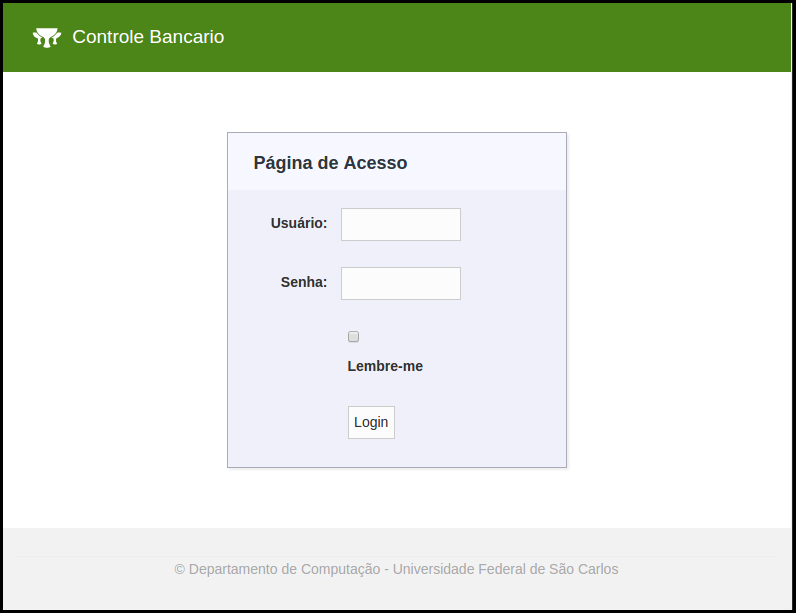
\includegraphics[width=14cm]{Login}
\caption{{\bf ControleBancario}: Página de {\it Login}}
\label{figExecutar}
\end{figure}

\section{Considerações finais}

\vspace{0.3cm}

Esse capítulo apresentou a segunda versão da implementação da aplicação {\bf
  ControleBancario}.         O        código-fonte        dessa        aplicação
({\footnotesize\texttt{ControleBancarioV2}})   encontra-se   disponível  em   um
repositório                      {\it                      GitHub}\footnote{URL:
  {\url{https://github.com/delanobeder/FG}}}.  

\vspace{0.2cm}

Dando continuidade ao desenvolvimento em  Grails, o próximo capítulo apresenta a
implementação   de  novas   funcionalidades  no   contexto  da   aplicação  {\bf
  ControleBancario}. 


%-------------------------------------------------------------------------------
%	CAPÍTULO 4
%-------------------------------------------------------------------------------

\chapter{Controle Bancário: Versão 3}\label{autorizacao}

Neste  capítulo,   dando  continuidade   ao  desenvolvimento  em   Grails,  será
apresentado o processo  de desenvolvimento da terceira versão  da aplicação {\bf
  ControleBancario}. Nessa versão são incorporadas as seguintes funcionalidades:

\begin{itemize}

\vspace{0.5cm}

\item Sintonia fina no controle de acesso:

\vspace{0.5cm}

\begin{itemize}

\vspace{0.5cm}

\item Atribuição de  papéis na criação das instâncias da  classe de domínio {\bf
  Gerente} e das instâncias das subclasses da classe {\bf Cliente}; 

\vspace{0.5cm}

\item Na segunda versão da  aplicação {\bf ControleBancario}, um cliente (físico
  ou jurídico)  pode acessar todas as  transações feitas em  contas (corrente ou
  poupança).  Na versão, discutida  nesse capítulo, clientes apenas terão acesso
  às transações realizadas nas contas (corrente ou poupança) a eles associadas;

\vspace{0.5cm}

\item  Se um  cliente possui  mais  de uma  conta (corrente  ou poupança),  será
  solicitado  que ele  escolha a  conta (corrente  ou poupança)  que  ele deseja
  acessar; 

\vspace{0.5cm}

\item Analogamente,  na segunda versão  da aplicação {\bf  ControleBancario}, um
  gerente  pode  acessar qualquer  conta  (corrente  ou  poupança).  Na  versão,
  discutida nesse capítulo, gerentes  apenas terão acesso às contas pertencentes
  à agência em que ele trabalha.

\end{itemize}

\vspace{0.5cm}

\item     Alteração     do    controlador     {\bf     Main},    definido     no
  Capítulo~\ref{autorizacao}, para refletir as mudanças relacionadas ao controle 
  de acesso;

\vspace{0.5cm}

\item  Alteração da  biblioteca  de marcas  {\it  LoginTagLibrary}, definida  no
  Capítulo~\ref{autorizacao}, para refletir as mudanças relacionadas ao controle
  de acesso; 

\vspace{0.5cm}

\item Acesso a um serviço {\it web}  que, dado um CEP como parâmetro, retorna as
  demais  informações de um  endereço (logradouro,  bairro, cidade,  etc). Essas
  informações  serão utilizadas  no  preenchimento automático  dos atributos  da
  classe de domínio {\bf Endereco}. 

\end{itemize}

\section{Configuração da aplicação} 

\vspace{0.5cm}

\noindent{\bf   Instalação   de    {\it   plugins}.}    Na   implementação   das
funcionalidades da aplicação  {\bf ControleBancario}, discutidas nesse capítulo,
será utilizado um  {\it plugin} Grails que adiciona  funcionalidades de clientes
REST. Ou seja,  ao utilizarmos esse {\it plugin}  será possível acessar serviços
web REST.\index{Plugins!rest} 

\vspace{0.2cm}

Conforme mencionado, desde  a versão 3 do Grails, a  inserção de dependências de
{\it  plugins} é  realizada no  arquivo  {\bf build.gradle}.   O conteúdo  desse
arquivo,  relacionado  à  configuração  de  dependências  de  {\it  plugins},  é
apresentado no Código~\ref{codBuildGradle3}.  

\vspace{0.2cm}

Dessa forma, para instalar  o plugin {\bf grails-datastore-rest-client} adicione
o comando \texttt{ compile "org.grails:grails-datastore-rest-client:5.0.0.RC2"},
descrevendo a  dependência, no arquivo {\bf  build.graddle} conforme apresentado
na linha 15 do Código~\ref{codBuildGradle3}. 

\begin{lstlisting}[numbers=left,  caption={\bf  build.gradle}, frame=trBL,
    float=htbp, label=codBuildGradle3, basicstyle =\footnotesize]
repositories {
    mavenLocal()
    maven { url "https://repo.grails.org/grails/core" }
}

dependencyManagement {
    imports {
        mavenBom "org.grails:grails-bom:$grailsVersion"
    }
    applyMavenExclusions false
}

dependencies {
    compile "org.springframework.boot:spring-boot-starter-logging"
    compile "org.springframework.boot:spring-boot-autoconfigure"
    compile "org.grails:grails-core"
    compile "org.springframework.boot:spring-boot-starter-actuator"
    compile "org.springframework.boot:spring-boot-starter-tomcat"
    compile "org.grails:grails-dependencies"
    compile "org.grails:grails-web-boot"
    compile "org.grails.plugins:cache"
    compile "org.grails.plugins:scaffolding"
    compile "org.grails.plugins:hibernate4"
    compile "org.hibernate:hibernate-ehcache"
    compile "org.grails.plugins:br-validation:0.3"
    compile "org.grails.plugins:spring-security-core:3.0.4"
    compile "org.grails:grails-datastore-rest-client:5.0.0.RC2"
    compile "org.grails.plugins:ajax-tags:1.0.0"
    console "org.grails:grails-console"
    profile "org.grails.profiles:web:3.1.4"
    runtime "org.grails.plugins:asset-pipeline"
    runtime "com.h2database:h2"
    runtime "org.postgresql:postgresql:9.3-1101-jdbc41"
    testCompile "org.grails:grails-plugin-testing"
    testCompile "org.grails.plugins:geb"
    testRuntime "org.seleniumhq.selenium:selenium-htmlunit-driver:2.47.1"
    testRuntime "net.sourceforge.htmlunit:htmlunit:2.18"
}
\end{lstlisting}

\section{Atribuição de papéis}

\vspace{0.5cm}

Na   segunda  versão   da   aplicação  {\bf   ControleBancario},  discutida   no
Capítulo~\ref{autenticacao}, os papéis são  atribuídos durante o {\it Bootstrap}
da aplicação  (Código~\ref{codBootStrap23}). Nessa terceira  versão da aplicação
{\bf ControleBancario}, a atribuição de papéis seguirá a abordagem discutida nas
próximas seções. 

\subsection{Classe de domínio Gerente X Papel {\bf ROLE\_GERENTE}}

\vspace{0.5cm}

Na  terceira   versão  da  aplicação   {\bf  ControleBancario},  o   papel  {\bf
  ROLE\_GERENTE} será atribuído automaticamente às todas instâncias da classe de
domínio {\bf Gerente}.  

\vspace{0.2cm}

Código~\ref{codSaveGerente}  mostra a  reimplementação da  ação {\bf  save()} do
controlador {\bf GerenteController} com o objetivo de atribuir automaticamente o 
papel  {\bf ROLE\_GERENTE}  a  todas as  instâncias  da classe  de domínio  {\bf
  Gerente}. Conforme  pode-se observar,  logo após a  operação de {\bf  save} na
instância  da classe  de  domínio  {\bf Gerente}  (linha~29),  essa instância  é
associada ao papel {\bf ROLE\_GERENTE} (linhas~31-33). 

\begin{lstlisting}[numbers=left,  caption=Controlador {\bf  Gerente}  (ação {\bf
      save()}), frame=trBL, float=htbp, label=codSaveGerente] 
package br.ufscar.dc.dsw

import static org.springframework.http.HttpStatus.*
import grails.transaction.Transactional
import org.springframework.security.access.annotation.Secured

@Secured('ROLE_ADMIN')
@Transactional(readOnly = true)
class GerenteController {

    static allowedMethods = [save: "POST", update: "PUT", delete: "DELETE"]

    // Demais a^çõ^es/m^é^todos do controlador GerenteController

    @Transactional
    def save(Gerente gerente) {
        if (gerente == null) {
            transactionStatus.setRollbackOnly()
            notFound()
            return
        }

        if (gerente.hasErrors()) {
            transactionStatus.setRollbackOnly()
            respond gerente.errors, view:'create'
            return
        }

        gerente.save flush:true

        def gerentePapel = Papel.findByAuthority("ROLE_GERENTE")
        
        UsuarioPapel.create(gerente, gerentePapel)
        
        request.withFormat {
            form {
                flash.message = message(code: 'default.created.message', 
                                        args: [message(code: 'gerente.label', 
                                        default: 'Gerente'), gerente.id])
                redirect gerente
            }
            '*' { respond gerente, [status: CREATED] }
        }
    }
}
\end{lstlisting}

\newpage

\subsection{Classe de domínio Cliente X Papel {\bf ROLE\_CLIENTE}}

\vspace{0.5cm}

Analógo  ao  discutido na  seção  anterior,  o  papel {\bf  ROLE\_CLIENTE}  será
atribuído  automaticamente  às todas  instâncias  das  subclasses  da classe  de
domínio abstrata {\bf Cliente}.

\begin{lstlisting}[caption=Controlador {\bf  ClienteFisico} (ação {\bf save()}),
    frame=trBL, float=htbp, label=codSaveFisico] 
class ClienteFisicoController {

    // Demais a^çõ^es/atributos/m^é^todos do controlador ClienteFisicoController

    @Transactional
    def save(ClienteFisico clienteFisico) {
        if (clienteFisico == null) {
            transactionStatus.setRollbackOnly()
            notFound()
            return
        }
        if (clienteFisico.hasErrors()) {
            transactionStatus.setRollbackOnly()
            respond clienteFisico.errors, view:'create'
            return
        }
        clienteFisico.enabled = false       
        clienteFisico.save flush:true
        def clientePapel = Papel.findByAuthority("ROLE_CLIENTE")
        UsuarioPapel.create(clienteFisico, clientePapel)
        request.withFormat {
            form {
                flash.message = message(code:'default.created.message', args: [message(code:'clienteFisico.label', 
                                        default: 'ClienteFisico'), clienteFisico.id])
                redirect clienteFisico
            }
            '*' { respond clienteFisico, [status: CREATED] }
        }
    }
}
\end{lstlisting}

\hyphenation{ClienteFisicoController}

Códigos~\ref{codSaveFisico}~e~\ref{codSaveJuridico} apresentam a reimplementação
da  ação {\bf  save()} dos  controladores {\bf  ClienteFisicoController}  e {\bf
  ClienteJuridicoController} com o objetivo  de atribuir automaticamente o papel
{\bf  ROLE\_CLIENTE}   a  todas  as   instâncias  da  classe  de   domínio  {\bf
  ClienteFisico} e {\bf ClienteJuridico}.  

\begin{lstlisting}[caption=Controlador   {\bf    ClienteJuridico}   (ação   {\bf
      save()}), frame=trBL, float=htbp, label=codSaveJuridico] 
class ClienteJuridicoController {

    // Demais a^çõ^es/atributos/m^é^todos do controlador ClienteJuridicoController

    @Transactional
    def save(ClienteJuridico clienteJuridico) {
        if (clienteJuridico == null) {
            transactionStatus.setRollbackOnly()
            notFound()
            return
        }
        if (clienteJuridico.hasErrors()) {
            transactionStatus.setRollbackOnly()
            respond clienteJuridico.errors, view:'create'
            return
        }
        clienteJuridico.enabled = false
        clienteJuridico.save flush:true
        def clientePapel = Papel.findByAuthority("ROLE_CLIENTE")
        UsuarioPapel.create(clienteJuridico, clientePapel)
        request.withFormat {
            form {
                flash.message = message(code:'default.created.message',args: [message(code:'clienteJuridico.label', 
                                        default: 'ClienteJuridico'), clienteJuridicoInstance.id])
                redirect clienteJuridico
            }
            '*' { respond clienteJuridico, [status: CREATED] }
        }
    }
}
\end{lstlisting}

\newpage

\section{Controle de acesso: Transações}

\vspace{0.5cm}

Conforme  discutido no  Capítulo~\ref{autenticacao},  o acesso  às transações  é
restrito aos  usuários que desempenham  o papel {\bf ROLE\_CLIENTE}.  Porém essa
abordagem  não é suficiente  pois um  cliente pode  acessar todas  as transações
realizadas em contas (corrente ou poupança) independentemente se essa conta está
associada ou não a esse cliente.

\vspace{0.2cm}

Na  versão  da  aplicação  {\bf  ControleBancario},  discutida  nesse  capítulo,
clientes  apenas  terão  acesso  às  transações  realizadas  nas  contas  a  ele
associadas.  

\subsection{Controlador: MainController}

\vspace{0.5cm}

Conforme discutido, o controlador {\bf  MainController}, em conjunto com a visão
{\bf  index}   associada,  consiste  na  página  principal   da  aplicação  {\bf
  ControleBancario}. 

\vspace{0.2cm}

Código~\ref{codMainController2}  apresenta   a  reimplementação  da   ação  {\bf
  index()} do  controlador {\bf  MainController} com o  objetivo de  refletir as
mudanças relacionadas  a nova  abordagem de controle  de acesso  discutida nesse
capítulo. 

\begin{lstlisting}[caption=Controlador    {\bf    MainController},   frame=trBL,
    float=htbp, label=codMainController2, numbers=left] 
package br.ufscar.dc.dsw

import org.springframework.security.access.annotation.Secured

@Secured(['ROLE_ADMIN', 'ROLE_CLIENTE', 'ROLE_GERENTE'])
class MainController {

    def springSecurityService

    def index() {

        def usuario = springSecurityService.getCurrentUser()
        def userName = springSecurityService.authentication.principal.getUsername()
        def authority = usuario.getAuthorities()[0].getAuthority()
        
        if (authority.equals('ROLE_GERENTE')) {
            def gerente = Gerente.findByUsername(userName)
            if (!session.agencia) {
                session.agencia = gerente.agencia
            }
        } else if (authority.equals('ROLE_CLIENTE')) {

            session.cliente = Cliente.findByUsername(userName)

            if (!session.conta) {
                if (session.cliente.contasCliente.size() == 1) {
                    def contaCliente = session.cliente.contasCliente[0]
                    session.contaCliente = contaCliente
                    session.conta = contaCliente.conta
                    session.agencia = session.conta.agencia
                } else {
                    redirect(controller:'selecionaConta')
                }
            }
        }        
    }
}
\end{lstlisting}

Quando um usuário acessa uma aplicação  {\it web}, ele estabelece uma sessão com
o servidor.  Uma variável de sessão existe  desde o instante de  sua criação até
que ela expire por inatividade, seja voluntariamente ({\it logout} da aplicação)
ou finalizado pela  aplicação.  Dessa forma, uma variável de  sessão é visível a
todos os controladores e visões enquanto não expirar por inatividade. 

\newpage

Conforme pode-se observar, quatro variáveis de sessão são utilizadas: 

\vspace{0.2cm}

\begin{itemize}

\item A  variável de sessão {\bf agencia}  armazena a agência em  que trabalha o
  usuário {\it logado}, caso este  desempenhe o papel {\bf ROLE\_GERENTE} (linha
  19); 

\vspace{0.2cm}

\item A variável  de sessão {\bf cliente} armazena o  usuário {\it logado}, caso
  este desempenhe o papel {\bf ROLE\_CLIENTE} (linha 23); 

\vspace{0.2cm}

\item  A  variável  de  sessão  {\bf  contaCliente}  armazena  a  conta  cliente
  (instância  da  classe de  domínio  {\bf  ContaCliente})  que o  usuário  {\it
  logado}, caso este  desempenhe o papel {\bf ROLE\_CLIENTE},  está acessando no
  momento.  As variáveis de sessão {\bf conta} e {\bf agencia} armazenam a conta
  (e a respectiva  agência) associada à conta cliente  armazenada na variável de
  sessão {\bf contaCliente};

\vspace{0.2cm}

\item É importante observar que se o cliente possuir apenas uma conta associada,
  este já será  armazenado na variável de sessão  {\bf contaCliente} (linha 28).
  Caso   contrário,   há   um   redirecionamento   para   o   controlador   {\bf
    SelecionaContaController} (linha 32).  

\end{itemize}

\subsection{Biblioteca de marcas: LoginTagLib}

\vspace{0.2cm}

No Código~\ref{codTagLib2}  tem-se a biblioteca de marcas  {\bf LoginTagLib} que
foi reimplementada para refletir as alterações discutidas nesse capítulo.  

\vspace{0.2cm}

Conforme pode-se observar essa classe  imprime o nome do papel desempenhado pelo
usuário {\it logado}  (linha 30).  Além disso, essa classe imprime  a conta (e a
respectiva agência) que o usuário  {\it logado} está acessando, considerando que
esse desempenhe o  papel {\bf ROLE\_CLIENTE} (variáveis de  sessão {\bf conta} e
{\bf agencia}, linhas  14--22). Por fim, essa classe imprime a  agência em que o
usuário {\it logado} trabalha, caso  esse desempenhe o papel {\bf ROLE\_GERENTE}
(variável de sessão {\bf agencia}, linhas 23--27).  

\begin{lstlisting}[caption=Biblioteca  de marca  {\bf  LoginTagLib}, frame=trBL,
    float=htbp, label=codTagLib2, numbers=left] 
class LoginTagLib {
    def springSecurityService
    def loginControl = {
        if (springSecurityService.isLoggedIn()) {
            def usuario = springSecurityService.getCurrentUser()
            def authority = usuario.getAuthorities()[0].getAuthority()
            def papel
            def span = "<span style=\"text-align:center;padding-left:25px;padding-right:25px\">"
            StringBuilder sb = new StringBuilder();
            if (authority.equals('ROLE_ADMIN')) {
                papel = "Administrador"
            } else if (authority.equals('ROLE_CLIENTE')) {
                papel = "Cliente"
                if (session.conta) {
                    sb.append("Conta: ")
                    sb.append(session.conta)
                    sb.append(" [")
                    session.agencia.attach()
                    sb.append(session.agencia)
                    sb.append("]")
                    sb.append(span)
                }
            } else {
                papel = "Gerente"
                sb.append("Ag^ê^ncia: ")
                sb.append(session.agencia)
            }
            out << span
            out << papel
            out << "</span>"
            out << span
            out << sb
            out << "</span>"
            out << "<span style=\"padding-right:25px\">"
            out << """ [${link(controller: "logout"){"Logout"}}]"""
            out << "</span>"
        }
    }
}
\end{lstlisting}

\subsection{Controlador: SelecionaContaController}\label{secSeleciona}

\vspace{0.2cm}

Caso um  cliente possua  mais de  uma conta (corrente  ou poupança),  ele deverá
escolher que  conta (corrente  ou poupança) ele  deseja acessar.   O controlador
{\bf SelecionaContaController}  é responsável  por essa nova  funcionalidade.  A
implementação      desse     controlador     encontra-se      apresentada     no
Código~\ref{codSelecionaContaController}.  

\vspace{0.2cm}

\begin{itemize}

\item  A ação  {\bf index()}  simplesmente  invoca implicitamente  a visão  {\bf
  index.gsp} que será discutida na próxima seção; e

\vspace{0.2cm}

\item A ação {\bf selected()} é  responsável por: (1) receber, como parâmetro, a
  conta escolhida pelo  usuário {\it logado} e armazenar  essa conta na variável
  de  sessão  {\bf  contaCliente}  e   (2)  redirecionar  a  requisição  para  o
  controlador {\bf MainController}. 

\end{itemize}

\begin{lstlisting}[caption=Controlador      {\bf      SelecionaContaController},
    frame=trBL, float=htbp, label=codSelecionaContaController] 
package br.ufscar.dc.dsw 
import org.springframework.security.access.annotation.Secured

@Secured('ROLE_CLIENTE')
class SelecionaContaController {

    def index() { }
    
    def selected() {
        def contaCliente = ContaCliente.get(params.conta)
        session.contaCliente = contaCliente
        session.conta = contaCliente.conta
        session.agencia = session.conta.agencia
        redirect(controller:'main')        
    }
}
\end{lstlisting}

\subsection{Visão: selecionaConta/index.gsp}

\vspace{0.5cm}

Relembrando   a   discussão  da   Seção~\ref{secEstatico},   para  cada   método
correspondente a  uma ação em um  controlador é criada  uma correspondente visão
(arquivo  com  extensão {\bf  .gsp}).   Assim, a  ação  {\bf  index()}, de  {\bf
  SelecionaContaController}, tem o correspondente {\bf index.gsp}.  

\begin{lstlisting}[caption=Visão   {\bf  selecionaConta/index.gsp},  frame=trBL,
    float=htbp, label=codSelecionaContaIndex] 
<%@ page import="br.ufscar.dc.dsw.ContaCliente" %>
<!DOCTYPE html>
<html>
    <head> 
        <meta name="layout" content="main"> 
    </head>
    <body>
        <div id="status" role="complementary">
            <h1>Selecione Conta:</h1>
            <g:form url="[action:'selected']" >
                <g:set var="contas" value="${ContaCliente.findAll("from ContaCliente as contaCliente where contaCliente.cliente = ?", [session.cliente])}" />
                <g:select name="conta" from="${contas}" 
                    optionKey="id" optionValue="conta">
                </g:select>
                </br> </br>
                <fieldset class="buttons">
                    <g:submitButton name="OK" class="save" value="OK" />
                </fieldset>
            </g:form>
        </div>
    </body>
</html>
\end{lstlisting}

A visão  {\bf index.gsp}  cria um formulário  HTML com  um campo de  seleção que
contém as contas clientes associadas ao cliente {\it logado} (variável de sessão
{\bf cliente}).  É  importante salientar que a submissão  do formulário invoca a
ação   {\bf   selected()}    do   controlador   {\bf   SelecionaContaController}
(Seção~\ref{secSeleciona}). A implementação  dessa visão encontra-se apresentada
no Código~\ref{codSelecionaContaIndex}.

\subsection{Classe de Domínio: Transacao}

\vspace{0.2cm}

Código~\ref{codTransacao2} mostra  a reimplementação  da classe de  domínio {\bf
  Transacao} com o  objetivo de refletir as mudanças  discutidas nesse capítulo.
Por questão de brevidade, apenas serão apresentadas as mudanças realizadas nessa
classe  de domínio.  Conforme  pode-se observar,  foram definidos  dois métodos:
{\bf  getValorReal()}  e  {\bf  getValorAnterior()}. Esses  dois  métodos  serão
utilizados  pelas  ações  {\bf  save()},  {\bf update()}  e  {\bf  delete()}  do
controlador {\bf TransacaoController}.  

\begin{lstlisting}[caption=Classe  de  domínio {\bf  Transacao},  frame =  trBL,
    float=htbp, label=codTransacao2] 
class Transacao {
    
    // Demais atributos/m^é^todos da classe de dom^í^nio Transacao
    static transients = ['valorAnterior', 'valorReal']
    
    double getValorReal() { // Retorna valor negativo caso transa^çã^o seja um d^é^bito
        return (tipo == D^É^BITO) ? -valor : valor;
    }
    
    double getValorAnterior() {
        def ant = this.getPersistentValue('valor') // Retorna o valor do atributo 'valor' antes de ser persistido
        def tipo = this.getPersistentValue('tipo') // Retorna o valor do atributo 'tipo' antes de ser persistido
        if (tipo == Transacao.D^É^BITO) {
            ant = -ant // Retorna valor negativo caso transa^çã^o seja um d^é^bito
        }
        return ant
    } 
}
\end{lstlisting}

\subsection{Controlador: TransacaoController}\label{secTransacaoController2}

\vspace{0.2cm}

Código~\ref{codTransacaoController3}  mostra  a  reimplementação do  controlador
{\bf TransacaoController} com o objetivo  de refletir as mudanças relacionadas a
nova abordagem de  controle de acesso discutida nesse  capítulo.  Por questão de
brevidade, apenas serão apresentadas as mudanças realizadas nesse controlador.  

Relembrando  a  discussão  da  Seção~\ref{secTransacaoController}, a  ação  {\bf
  index()} é responsável por retornar a lista de instâncias da classe de domínio
{\bf Transacao}.  No caso da implementação apresentada nesse capítulo, a lista é
composta  apenas  pelas  transações  que  foram realizadas  na  conta  escolhida
anteriormente pelo usuário {\it logado} (variável de sessão {\bf contaCliente}).  

A ação {\bf create()} é responsável por criar uma instância da classe de domínio
{\bf Transacao} que  é repassada (retornada) para a  visão {\bf create.gsp} (uma
página que contem  um formulário HTML). Quando o formulário  é submetido, a ação
{\bf save()} valida  os dados e caso, tenha sucesso, grava  a instância no banco
de dados e  redireciona para a ação  {\bf show()}.  Por outro lado,  se os dados
são inválidos, a ação {\bf  save()} renderiza a visão {\bf create.gsp} novamente
para  que o  usuário  corriga os  erros  encontrados na  validação.  No caso  da
implementação apresentada nesse capítulo, a transação criada é associada à conta
escolhida  anteriormente pelo  usuário  {\it logado}  (variável  de sessão  {\bf
  contaCliente}).  

Analogamente, a  ação {\bf edit()} é  responsável por recuperar  uma instância a
ser atualizada  posteriormente.  A instância recuperada  é repassada (retornada)
para a visão {\bf edit.gsp} (uma página que contém um formulário HTML). Quanto o
formulário é  submetido o método  {\bf update()} valida  os dados e  caso, tenha
sucesso, atualiza a  instância no banco de dados e redireciona  para a ação {\bf
  show()}.  Por  outro lado, se  os dados são  inválidos, a ação  {\bf update()}
renderiza a visão  {\bf edit.gsp} novamente para que o  usuário corriga os erros
encontrados na  validação.  É importante salientar  que as ações  {\bf save()} e
{\bf  update()}  atualizam  o  saldo   da  conta  para  refletir  as  transações
criadas e/ou atualizadas. 

\begin{lstlisting}[caption=Controlador  {\bf  TransacaoController},  frame=trBL,
    float=htbp, label=codTransacaoController3] 
class TransacaoController {

    // Demais a^çõ^es/atributos/m^é^todos do controlador TransacaoController

    def index(Integer max) {
        params.max = Math.min(max ?: 10, 100)
        def results = Transacao.findAllByContaCliente(session.contaCliente, params)
        respond results, model:[transacaoCount: Transacao.count()]
    }

    @Transactional
    def save(Transacao transacao) {
        if (transacao == null) {
            transactionStatus.setRollbackOnly()
            notFound()
            return
        }
        if (transacao.hasErrors()) {
            transactionStatus.setRollbackOnly()
            respond transacao.errors, view:'create'
            return
        }
        def conta = transacao.contaCliente.conta
        conta.saldo += transacao.getValorReal()
        transacao.save flush:true
        conta.save flush: true
        request.withFormat {
            form multipartForm {
                flash.message = message(code: 'default.created.message', args:[message(code: 'transacao.label', 
                                        default: 'Transacao'), transacao.id])
                redirect transacao
            }
            '*' { respond transacao, [status: CREATED] }
        }
    }

    def edit(Transacao transacao) {
        if (transacao != null && transacao.contaCliente.id != session.contaCliente.id) {
            flash.message = message(code: 'springSecurity.denied.message', args: [message(code: 'transacao.label', 
                                    default: 'Transacao'), transacao.id])
            redirect action: "index"
        }
        respond transacaoInstance
    }

    @Transactional
    def update(Transacao transacao) {
        if (transacao == null) {
            transactionStatus.setRollbackOnly()
            notFound()
            return
        }
        if (transacao.hasErrors()) {
            transactionStatus.setRollbackOnly()
            respond transacao.errors, view:'edit'
            return
        }
        def conta = transacao.contaCliente.conta
        conta.saldo += (transacao.getValorReal() - transacao.getValorAnterior())
        transacao.save flush:true
        conta.save flush: true
        request.withFormat {
            form multipartForm {
                flash.message = message(code: 'default.updated.message', args: [message(code: 'transacao.label', 
                                        default: 'Transacao'), transacao.id])
                redirect transacao
            }
            '*'{ respond transacao, [status: OK] }
        }
    }
    
    @Transactional
    def delete(Transacao transacao) {
        if (transacao.contaCliente.id != session.contaCliente.id) {
            flash.message = message(code: 'springSecurity.denied.message', args: [message(code: 'transacao.label', 
                                    default: 'Transacao'), transacao.id])
            redirect action: "index", method: "GET"
            return
        }
        if (transacao == null) {
            transactionStatus.setRollbackOnly()
            notFound()
            return
        }
        def conta = transacao.contaCliente.conta;
        conta.saldo -= transacao.getValorReal()
        transacao.delete flush:true
        conta.save flush:true
        request.withFormat {
            form multipartForm {
                flash.message = message(code: 'default.deleted.message', args: [message(code: 'transacao.label', 
                                        default: 'Transacao'), transacao.id])
                redirect action:"index", method:"GET"
            }
            '*'{ render status: NO_CONTENT }
        }
    }
}
\end{lstlisting}

\newpage

Relembrando  a discussão da  Seção~\ref{secURL}, Grails  usa uma  convenção para
automaticamente configurar o caminho para uma ação em particular. Por exemplo, a
URL \url{http://localhost:8080/transacao/edit/1} executaria  a ação {\bf edit()}
na instância da classe de domínio {\bf Transacao} cujo {\bf id} é igual a 1. 

\vspace{0.2cm}

Dessa forma, através da digitação de  uma URL no navegador {\it web}, um cliente
{\it logado} pode editar ou remover indevidamente (maliciosamente) uma transação
não associada a nenhuma de suas  contas. Nesse contexto, as ações {\bf edit()} e
{\bf delete()}  foram alteradas  com o objetivo  de prevenir  essas atualizações
indevidas.  Por  fim, a  ação {\bf  delete()} também atualiza  o saldo  da conta
associada (crédito ou débito) para refletir a operação de remoção da transação.

\subsection{Template transacao/\_fields.gsp}

\vspace{0.5cm}

Essa   seção   apresenta   o   {\it   template}   {\bf   transacao/\_fields.gsp}
(Código~\ref{codTransacaoFields})   que   será   utilizado  pela   visões   {\bf
  create.gsp}  e {\bf  edit.gsp} e  que  contém personalizações  na entrada  dos
atributos {\bf contaCliente}  e {\bf caixaEletronico} da classe  de domínio {\bf
  Transacao}.  Essas  personalizações  tem   como  objetivo  refletir  as  novas
funcionalidades discutidas nesse capítulo.  

\begin{lstlisting}[caption={\it     Template}     {\bf    transacao/\_fields.gsp},
    frame=trBL, float=htbp, label=codTransacaoFields, numbers=left]
<%@ page import="br.ufscar.dc.dsw.CaixaEletronico" %>
<%@ page import="br.ufscar.dc.dsw.Transacao" %>

<div class="fieldcontain ${hasErrors(bean: transacaoInstance, field: 'contaCliente', 'error')} required">
    <label for="contaCliente">
        <g:message code="transacao.contaCliente.label" default="Conta Cliente"/>
        <span class="required-indicator">*</span>
    </label>
    <g:select id="contaCliente" name="contaCliente.id" from="${session.contaCliente}" optionKey="id"
              value="${transacaoInstance?.contaCliente?.id}" class="many-to-one"/>
</div>

<div class="fieldcontain ${hasErrors(bean: transacaoInstance, field: 'caixaEletronico', 'error')} ">
    <label for="caixaEletronico">
        <g:message code="transacao.caixaEletronico.label" default="Caixa Eletronico"/>
        <span class="required-indicator">*</span>
    </label>
    <g:set var="caixas"
           value="${CaixaEletronico.findAll("from CaixaEletronico as caixa where caixa.banco = ?", 
                                             [session.agencia.banco])}"/>
    <g:select id="caixaEletronico" name="caixaEletronico.id" from="${caixas}" optionKey="id"
              value="${transacaoInstance?.caixaEletronico?.id}" class="many-to-one"/>
</div>
\end{lstlisting}

Conforme pode-se  observar, a transação  criada/editada sempre será  associada à
conta   escolhida    anteriormente   pelo   usuário    (variável   sessão   {\bf
  contaCliente}). Ou seja, o atributo {\bf from} (linha 9) do campo de seleção é
limitado ao valor armazenado na variável de sessão {\bf contaCliente}. 

\vspace{0.2cm}

De  maneira  análoga,  o  segundo   campo  de  seleção  (linhas  21--22)  apenas
possibilita que o usuário selecione caixas eletrônicos pertencentes ao banco que
mantém  a  conta (variável  de  sessão  {\bf  contaCliente}) sendo  acessada  no
momento.   É importante  salientar  que o  atributo  {\bf from}  desse campo  de
seleção é a variável {\bf caixas} que armazena uma lista de instâncias da classe
de domínio {\bf CaixaEletronico} obtida através da execução de uma consulta {\bf
  findAll()} (linhas 19--20) parametrizada. O parâmetro dessa consulta é o banco 
que mantém a conta sendo acessada no momento. 

\vspace{0.2cm}

Código~\ref{codTransacaoCreate}   mostra  a   reimplementação   da  visão   {\bf
  transacao/create.gsp}. Por questão de  brevidade, apenas serão apresentadas as
mudanças realizadas  nessa visão.   Pode-se observar que  o {\it  template} {\bf
  \_fields.gsp} é renderizado (linha 17) no contexto do formulário HTML definido 
pela {\it  tag} {\bf  g:form} (linhas 15--25).   Dessa forma, os  atributos {\bf
  contaCliente} e  {\bf caixaEletronico} são incluídos no  formulário através da
renderização  do  {\it  template}  {\bf  \_fields.gsp} enquanto  os  demais  são
incluídos através da {\it tag} {\bf f:all} (linha 19).  

\begin{lstlisting}[caption={\bf    transacao/create.gsp},
    frame=trBL, float=htbp, label=codTransacaoCreate, numbers=left]
<div id="create-transacao" class="content scaffold-create" role="main">
    <h1><g:message code="default.create.label" args="[entityName]"/></h1>
    <g:if test="${flash.message}">
        <div class="message" role="status">${flash.message}</div>
    </g:if>
    <g:hasErrors bean="${this.transacao}">
        <ul class="errors" role="alert">
            <g:eachError bean="${this.transacao}" var="error">
                <li <g:if test="${error in org.springframework.validation.FieldError}">
                                 data-field-id="${error.field}"</g:if>><g:message
                        error="${error}"/></li>
            </g:eachError>
        </ul>
    </g:hasErrors>
    <g:form action="save">
        <fieldset class="form">
            <g:render template="fields"/>

            <f:all bean="transacao" except="contaCliente, caixaEletronico"/>
        </fieldset>
        <fieldset class="buttons">
            <g:submitButton name="create" class="save"
                            value="${message(code: 'default.button.create.label', default: 'Create')}"/>
        </fieldset>
    </g:form>
</div>
\end{lstlisting}

\begin{remark}
Análogo  à visão  {\bf transacao/create.gsp},  a visão  {\bf transacao/edit.gsp}
também   necessita  ser   alterada   para  utilizar   o   {\it  template}   {\bf
  \_fields.gsp}. Fica como exercício para o leitor realizar tal alteração.
\end{remark}

\subsection{Executando a aplicação}

\vspace{0.5cm}

Após realizar  as alterações discutidas  nessa seção, sugere-se que  a aplicação
{\bf ControleBancario} seja executada. 

\vspace{0.2cm}

Figura~\ref{figPageCliente} apresenta  a página principal  conforme acessada por
um usuário {\it logado} que desempenha o papel {\bf ROLE\_CLIENTE}. 

\begin{figure}[htbp]
\centering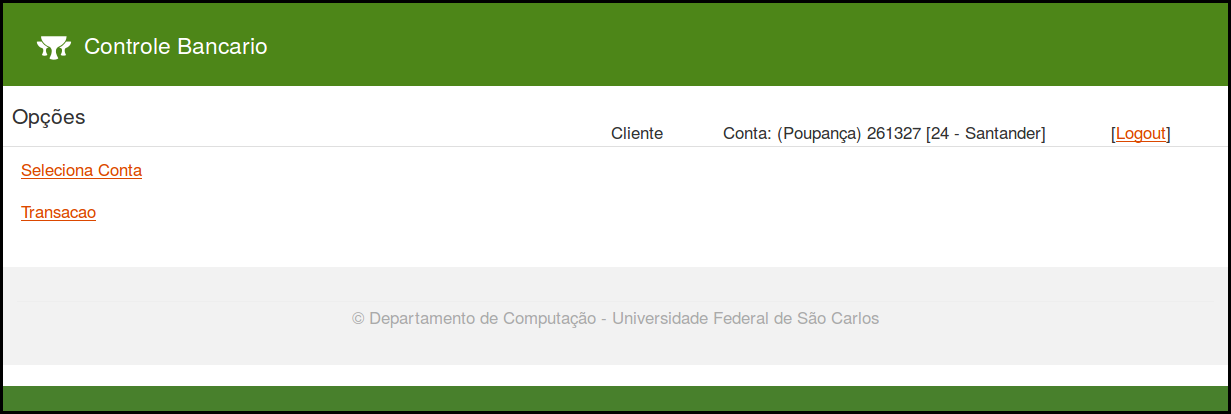
\includegraphics[width=14cm]{pageCliente}
\caption{Visão {\bf main/index.gsp}: {\bf ROLE\_CLIENTE}}
\label{figPageCliente}
\end{figure}

Conforme pode-se  observar o  usuário {\it logado}  tem duas  opções disponíveis
(dois controladores da aplicação {\bf ControleBancario}):

\vspace{0.3cm}

\begin{itemize}

\item {\bf SelecionaConta} caso deseje escolher que conta (corrente ou poupança)
  ele deseja acessar;

\vspace{0.3cm}

\item  {\bf  Transacao} caso  deseje  acessar/atualizar  a  lista de  transações
  realizadas    na    conta    que    está   sendo    acessada    no    momento.
  Figura~\ref{indexTransacaoFig}  apresenta a lista  de transações  associadas a
  uma conta do usuário {\it logado}.  

\end{itemize}

\begin{figure}[htbp]
\centering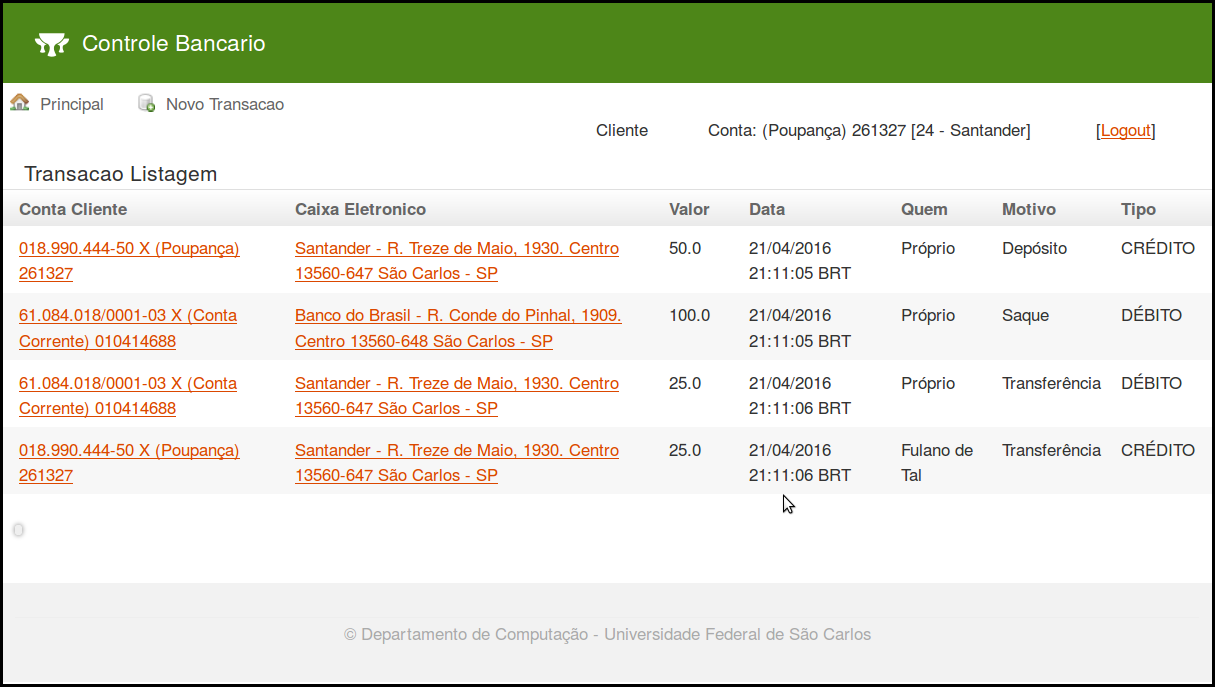
\includegraphics[width=14cm]{indexTransacao}
\caption{Lista de transações de uma conta do usuário {\it logado}}
\label{indexTransacaoFig}
\end{figure}

\section{Controle de acesso: Contas}

\vspace{0.5cm}

Conforme discutido no Capítulo~\ref{autenticacao}, o acesso às contas é restrito
aos usuários que desempenham o  papel {\bf ROLE\_GERENTE}.  Porém essa abordagem
não  é suficiente  pois um  gerente pode  acessar todas  as contas  (corrente ou
poupança) independentemente se essa conta pertence ou não a sua agência.

\vspace{0.2cm}

Na  versão  da  aplicação  {\bf  ControleBancario},  discutida  nesse  capítulo,
gerentes  apenas  terão acesso  às  contas pertencentes  à  agência  em que  ele
trabalha. 

\subsection{Controlador: ContaCorrenteController}

\vspace{0.5cm}

Código~\ref{codContaCorrenteController}    apresenta   a    reimplementação   do
controlador {\bf ContaCorrenteController} com o objetivo de refletir as mudanças
relacionadas a nova abordagem de controle de acesso discutida nesse capítulo.  

\vspace{0.2cm}

Relembrando  a  discussão  da  Seção~\ref{secTransacaoController}, a  ação  {\bf
  index()} é responsável por retornar a lista de instâncias da classe de domínio
{\bf  ContaCorrente}.  No caso  da implementação  apresentada nesse  capítulo, a
lista é composta apenas pelas contas  correntes que pertencem à agência em que o
usuário {\it logado} trabalha (variável de sessão {\bf agencia}). 

\vspace{0.2cm}

Por  fim,  relembrando  a  discussão da  Seção~\ref{secTransacaoController2},  é
possível que  gerentes {\it logados}  acessem de forma indevida  (maliciosa) uma
conta não  associada à agência  em que trabalha.  Nesse contexto, as  ações {\bf
  edit()}  e {\bf delete()}  foram alteradas  com o  objetivo de  prevenir essas
atualizações indevidas.

\vspace{0.5cm}

\begin{remark}
Análogo    ao     controlador    {\bf    ContaCorrenteController},     o    {\bf
  ContaPoupancaController}  também  necessita  ser  alterado  para  refletir  as
mudanças relacionadas  a nova  abordagem de controle  de acesso  discutida nesse
capítulo. Fica como exercício para o leitor realizar tal alteração. 
\end{remark}

\newpage

\begin{lstlisting}[caption=Controlador       {\bf      ContaCorrenteController},
    frame=trBL, float=htbp, label=codContaCorrenteController] 
class ContaCorrenteController {

    // Demais a^çõ^es/atributos/m^é^todos do controlador ContaCorrenteController

    def index(Integer max) {
        params.max = Math.min(max ?: 10, 100)        

        def results = ContaCorrente.findAllByAgencia(session.agencia, params)

        respond results, model:[contaCorrenteCount: ContaCorrente.count()]
    }

    def edit(ContaCorrente contaCorrente) {
        
        if (contaCorrente != null && contaCorrente.agencia.id != session.agencia.id) {
            flash.message = message(code: 'springSecurity.denied.message', args: [message(code: 
                                    'contaCorrente.label', default: 'ContaCorrente'), contaCorrente.id])
            redirect action: "index"
        }

        respond contaCorrente
    }

    @Transactional
    def delete(ContaCorrente contaCorrente) {
        
        if (contaCorrente.agencia.id != session.agencia.id) {
            flash.message = message(code: 'springSecurity.denied.message', args: [message(code: 
                                    'contaCorrente.label', default: 'ContaCorrente'), contaCorrente.id])
            redirect action: "index"
            return
        }

        if (contaCorrente == null) {
            notFound()
            transactionStatus.setRollbackOnly()
            return
        }

        contaCorrente.delete flush:true

        request.withFormat {
            form {
                flash.message = message(code: 'default.deleted.message', args: [message(code: 
                                        'contaCorrente.label', default: 'ContaCorrente'), contaCorrente.id])
                redirect action:"index", method:"GET"
            }
            '*'{ render status: NO_CONTENT }
        }
    }
}
\end{lstlisting}

\subsection{Template contaCorrente/\_fields.gsp}

\vspace{0.5cm}

Essa   seção  apresenta  o   {\it  template}   {\bf  contaCorrente/\_fields.gsp}
(Código~\ref{codContaCorrenteFields})  que  será   utilizado  pela  visões  {\bf
  create.gsp}  e {\bf  edit.gsp} e  que contém  a personalização  na  entrada do
atributo {\bf agencia} da classe de domínio {\bf ContaCorrente}.  

\vspace{0.2cm}

Conforme pode-se observar, a conta corrente criada/editada sempre será associada
à agência  (variável de  sessão {\bf  agencia}) em que  trabalha o  usuário {\it
  logado}.

\vspace{0.5cm}

\begin{lstlisting}[caption={\it     Template}     {\bf    contaCorrente/\_fields.gsp},
    frame=trBL, float=htbp, label=codContaCorrenteFields]
<div class="fieldcontain ${hasErrors(bean: contaCorrente, field: 'agencia', 'error')} required">
    <label for="agencia">
        <g:message code="contaCorrente.agencia.label" default="Agencia"/>
        <span class="required-indicator">*</span>
    </label>
    <g:select id="agencia" name="agencia.id" from="${session.agencia}" optionKey="id" required=""
              value="${contaCorrente?.agencia?.id}" class="many-to-one"/>
</div>
\end{lstlisting}

\newpage

Código~\ref{codContaCorrenteCreate}  mostra  a  reimplementação  da  visão  {\bf
  contaCorrente/create.gsp}. Por questão de brevidade, apenas serão apresentadas
as mudanças realizadas nessa visão.  Pode-se observar que  o {\it  template} {\bf
  \_fields.gsp} é renderizado (linha 17) no contexto do formulário HTML definido 
pela  {\it tag}  {\bf g:form}  (linhas 15--25).   Dessa forma,  o  atributo {\bf
  agencia} é  incluído no formulário  através da renderização do  {\it template}
{\bf \_fields.gsp}  enquanto os demais são  incluídos através da  {\it tag} {\bf
  f:all} (linha 19).  

\begin{lstlisting}[caption={\bf    contaCorrente/create.gsp},
    frame=trBL, float=htbp, label=codContaCorrenteCreate, numbers=left]
<div id="create-contaCorrente" class="content scaffold-create" role="main">
    <h1><g:message code="default.create.label" args="[entityName]"/></h1>
    <g:if test="${flash.message}">
        <div class="message" role="status">${flash.message}</div>
    </g:if>
    <g:hasErrors bean="${this.contaCorrente}">
        <ul class="errors" role="alert">
            <g:eachError bean="${this.contaCorrente}" var="error">
                <li <g:if test="${error in org.springframework.validation.FieldError}">
                                 data-field-id="${error.field}"</g:if>><g:message
                        error="${error}"/></li>
            </g:eachError>
        </ul>
    </g:hasErrors>
    <g:form action="save">
        <fieldset class="form">
            <g:render template="fields"/>

            <f:all bean="contaCorrente" except="agencia"/>
        </fieldset>
        <fieldset class="buttons">
            <g:submitButton name="create" class="save"
                            value="${message(code: 'default.button.create.label', default: 'Create')}"/>
        </fieldset>
    </g:form>
</div>
\end{lstlisting}

\begin{remark}
Análogo    à    visão    {\bf    contaCorrente/create.gsp},   a    visão    {\bf
  contaCorrente/edit.gsp}  também necessita  ser alterada  para utilizar  o {\it
  template} {\bf \_fields.gsp}.  

Análogo  ao {\it  template} {\bf  contaCorrente/\_fields.gsp}, o  {\it template}
{\bf   contaPoupanca/\_fields.gsp}   (e    consequentemente   as   visões   {\bf
  contaPoupanca/create.gsp} e  {\bf contaPoupanca/edit.gsp}) também  precisa ser
definido com  o intuito de personalizar  a entrada do atributo  {\bf agencia} da
classe  de  domínio {\bf  ContaPoupanca}.  Fica  como  exercício para  o  leitor
realizar tais alterações.  
\end{remark}

\subsection{Controlador: ContaClienteController}

\vspace{0.2cm}

Código~\ref{codContaClienteController2}    apresenta   a    reimplementação   do
controlador {\bf ContaClienteController} com o objetivo de refletir as mudanças
relacionadas a nova abordagem de controle de acesso discutida nesse capítulo.  

\vspace{0.1cm}

\hyphenation{ContaCliente}

A ação {\bf index()} é responsável  por retornar a lista de instâncias da classe
de   domínio  {\bf   ContaCliente}   que  materializa   o  relacionamento   {\em
  muitos-para-muitos}  entre   as  classes  de   domínio  {\bf  Conta}   e  {\bf
  Cliente}. No caso da implementação apresentada nessa seção, a lista é composta
apenas pelas instâncias que estão associadas a contas que pertencem à agência em
que o usuário {\it logado} trabalha (variável de sessão {\bf agencia}).  

\vspace{0.1cm}

A ação {\bf save()} valida os dados  e caso, tenha sucesso, grava a instância no
banco de  dados. No caso da  implementação apresentada nessa seção,  a ação {\bf
  save()}  também habilita  o cliente  (torna-se um  usuário da  aplicação) caso
esteja desabilitado. No contexto da aplicação {\bf ControleBancario}, um cliente
apenas  torna-se  um  usuário (pode  realizar  a  operação  de {\it  login})  da
aplicação  caso  tenha  uma  conta  associada. Além  disso,  conforme  discutido
anteriormente, é possível  que gerentes {\it logados} acessem  de forma indevida
(maliciosa) instâncias dessa  classe de domínio.  Nesse contexto,  as ações {\bf
  edit()}  e {\bf delete()}  foram alteradas  com o  objetivo de  prevenir essas
atualizações indevidas.  

\begin{lstlisting}[caption=Controlador {\bf ContaClienteController}, frame=trBL,
    float=htbp, label=codContaClienteController2] 
class ContaClienteController {

    // Demais a^çõ^es/atributos/m^é^todos do controlador ContaClienteController

    def index(Integer max) {
        params.max = Math.min(max ?: 10, 100)
		
        def results = ContaCliente.findAll("from ContaCliente as cc where cc.conta.agencia = :agencia",
            [agencia: session.agencia])
		
        respond results, model:[contaClienteCount: ContaCliente.count()]
    }

    @Transactional
    def save(ContaCliente contaCliente) {
        if (contaCliente == null) {
            transactionStatus.setRollbackOnly()
            notFound()
            return
        }

        if (contaCliente.hasErrors()) {
            transactionStatus.setRollbackOnly()
            respond contaCliente.errors, view:'create'
            return
        }

        contaCliente.save flush:true
        def cliente = contaCliente.cliente
        if (!cliente.enabled) {
            cliente.enabled = true
            cliente.save flush:true
        }

        request.withFormat {
            form multipartForm {
                flash.message = message(code: 'default.created.message', args: [message(code: 'contaCliente.label', 
                                        default: 'ContaCliente'), contaCliente.id])
                redirect contaCliente
            }
            '*' { respond contaCliente, [status: CREATED] }
        }
    }

    def edit(ContaCliente contaCliente) {
        if (contaCliente != null && contaCliente.conta.agencia.id != session.agencia.id) {
            flash.message = message(code: 'springSecurity.denied.message', args: [message(code:
                    'contaCliente.label', default: 'ContaCliente'), contaCliente.id])
            redirect action: "index"
        }
        respond contaCliente
    }

    @Transactional
    def delete(ContaCliente contaCliente) {
        if (contaCliente != null && contaCliente.conta.agencia.id != session.agencia.id) {
            flash.message = message(code: 'springSecurity.denied.message', args: [message(code:
                    'contaCliente.label', default: 'ContaCliente'), contaCliente.id])
            redirect action: "index"
        }

        if (contaCliente == null) {
            transactionStatus.setRollbackOnly()
            notFound()
            return
        }
        contaCliente.delete flush: true

        request.withFormat {
            form multipartForm {
                flash.message = message(code: 'default.deleted.message', args: [message(code: 'contaCliente.label', default: 'ContaCliente'), contaCliente.id])
                redirect action: "index", method: "GET"
            }
            '*' { render status: NO_CONTENT }
        }
    }

}
\end{lstlisting}

\newpage

\subsection{Template contaCliente/\_fields.gsp}

\vspace{0.5cm}

Essa   seção  apresenta   o  {\it   template}   {\bf  contaCliente/\_fields.gsp}
(Código~\ref{codContaClienteFields})  que   será  utilizado  pela   visões  {\bf
  create.gsp}  e {\bf  edit.gsp} e  que  contém personalizações  na entrada  dos
atributos {\bf cliente} e {\bf conta} da classe de domínio {\bf ContaCliente}.  

\begin{lstlisting}[caption={\it   Template}   {\bf   contaCliente/\_fields.gsp},
    frame=trBL, float=htbp, label=codContaClienteFields, numbers=left] 
<%@ page import="br.ufscar.dc.dsw.Conta" %>
<%@ page import="br.ufscar.dc.dsw.ContaCliente" %>

<div class="fieldcontain ${hasErrors(bean: contaClienteInstance, field: 'cliente', 'error')} required">
    <label for="cliente">
        <g:message code="contaCliente.cliente.label" default="Cliente"/>
        <span class="required-indicator">*</span>
    </label>
    <g:select id="cliente" name="cliente.id" from="${br.ufscar.dc.dsw.Cliente.list()}" optionKey="id"
              required="" value="${contaClienteInstance?.cliente?.id}"
              disabled="${contaClienteInstance?.cliente?.id != null}" class="many-to-one"/>
</div>

<div class="fieldcontain ${hasErrors(bean: contaClienteInstance, field: 'conta', 'error')} required">
    <label for="conta">
        <g:message code="contaCliente.conta.label" default="Conta"/>
        <span class="required-indicator">*</span>
    </label>
    <g:set var="contas"
           value="${Conta.findAll("from Conta as conta where conta.agencia = ?", [session.agencia])}"/>
    <g:select id="conta" name="conta.id" from="${contas}" optionKey="id" required=""
              value="${contaClienteInstance?.conta?.id}"
              disabled="${contaClienteInstance?.conta?.id != null}" class="many-to-one"/>
</div>
\end{lstlisting}

Conforme pode-se  observar, os campos de  seleção dos atributos  {\bf cliente} e
{\bf conta} são desabilitados nas operações de edição (linhas 11 e 23) -- quando
o  relacionamento {\em  muitos-para-muitos}  entre as  classes  de domínio  {\bf
  Conta} e  {\bf Cliente}  já foi  estabelecido.  Ou seja,  na edição  apenas os
demais atributos podem  ser atualizados. Além disso, o  segundo campo de seleção
(linha 21) apenas possibilita que o usuário {\it logado} apenas possa selecionar
contas (corrente ou  poupança) pertencentes à agência em  que trabalha (variável
de sessão {\bf agencia}).  

\vspace{0.2cm}

Código~\ref{codContaClienteCreate}  mostra  a   reimplementação  da  visão  {\bf
  contaCliente/create.gsp}. Por questão  de brevidade, apenas serão apresentadas
as mudanças realizadas nessa visão.   Pode-se observar que o {\it template} {\bf
  \_fields.gsp} é renderizado (linha 3)  no contexto do formulário HTML definido
pela {\it  tag} {\bf g:form}.   Dessa forma, os  atributos {\bf cliente}  e {\bf
  conta} são incluídos  no formulário através da renderização  do {\it template}
{\bf \_fields.gsp}  enquanto os demais são  incluídos através da  {\it tag} {\bf
  f:all} (linha 5).  

\begin{lstlisting}[caption={\bf    contaCliente/create.gsp},
    frame=trBL, float=htbp, label=codContaClienteCreate, numbers=left]
<g:form action="save">
    <fieldset class="form">
        <g:render template="fields"/>

        <f:all bean="contaCliente" except="cliente, conta"/>
    </fieldset>

    <fieldset class="buttons">
        <g:submitButton name="create" class="save"
                        value="${message(code: 'default.button.create.label', default: 'Create')}"/>
    </fieldset>
</g:form>
\end{lstlisting}

\begin{remark}
Análogo    à    visão    {\bf    contaCliente/create.gsp},    a    visão    {\bf
  contaCliente/edit.gsp}  também necessita  ser  alterada para  utilizar o  {\it
  template} {\bf \_fields.gsp}.  Fica como exercício para o  leitor realizar tal
alteração. 
\end{remark}

\subsection{Controlador: ContaController}

\vspace{0.5cm}

Código~\ref{codContaController2} apresenta a reimplementação do controlador {\bf
  ContaController} com  o objetivo de  refletir as mudanças relacionadas  a nova
abordagem de controle de acesso discutida nesse capítulo.  

\vspace{0.2cm}

Relembrando  a  discussão  da  Seção~\ref{secTransacaoController}, a  ação  {\bf
  index()} é responsável por retornar a lista de instâncias da classe de domínio
{\bf Conta}.   No caso  da implementação apresentada  nesse capítulo, a  lista é
composta  apenas pelas  contas que  pertencem à  agência em  que o  usuário {\it
  logado} trabalha (variável de sessão {\bf agencia}).

\begin{lstlisting}[caption=Controlador    {\bf   ContaController},   frame=trBL,
    float=htbp, label=codContaController2] 
class ContaController {

    // Demais a^çõ^es/atributos/m^é^todos do controlador ContaController
    
    def index(Integer max) {
        params.max = Math.min(max ?: 10, 100)
        
        def results = Conta.findAllByAgencia(session.agencia, params)
                
        respond results, model:[list: results, contaInstanceCount: Conta.count()]
    }
    
    @Secured(['ROLE_ADMIN', 'ROLE_CLIENTE', 'ROLE_GERENTE'])
    def show() {
        Conta conta = Conta.get(params.id)
        if (conta.instanceOf(ContaCorrente)) {
            forward controller: 'contaCorrente', action: "show"
        } else {
            forward controller: 'contaPoupanca', action: "show"
        }
    }
}

\end{lstlisting}

\subsection{Executando a aplicação}

\vspace{0.5cm}

Figura~\ref{figPageGerente} apresenta  a página principal  conforme acessada por
um usuário {\it logado} que desempenha o papel {\bf ROLE\_GERENTE}. 

\vspace{0.2cm}

\begin{figure}[htbp]
\centering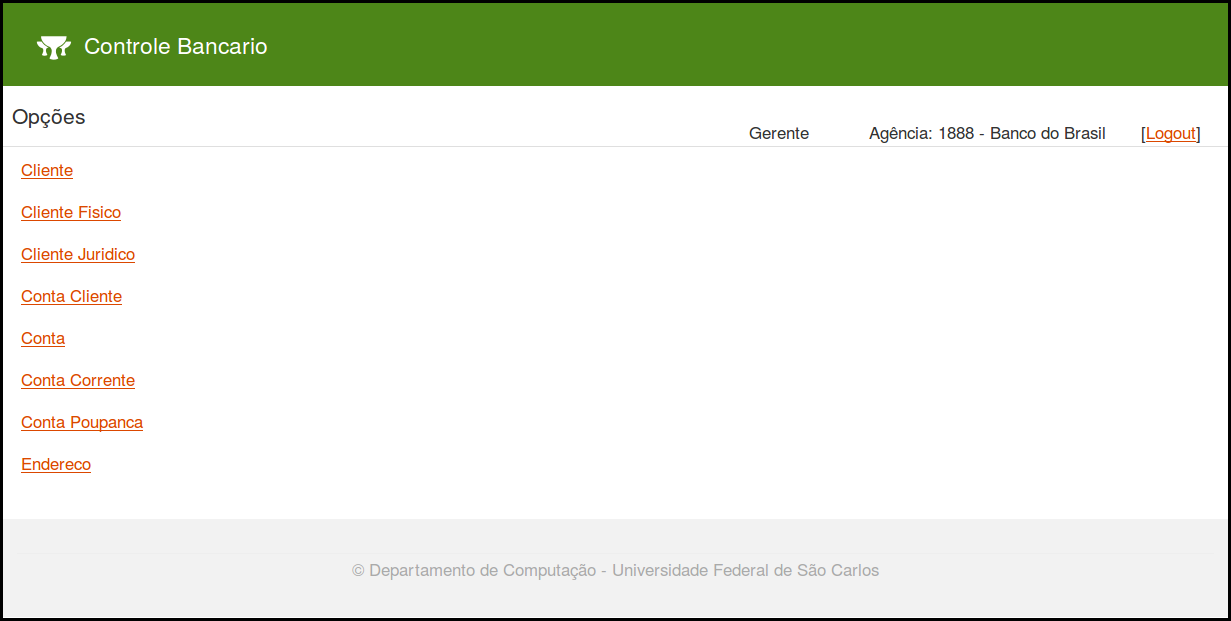
\includegraphics[width=14cm]{pageGerente}
\caption{Visão {\bf main/index.gsp}: {\bf ROLE\_GERENTE}}
\label{figPageGerente}
\end{figure}

Conforme pode-se  observar o  usuário {\it logado}  tem oito  opções disponíveis
(controladores da aplicação {\bf ControleBancario}): 

\vspace{0.4cm}

\begin{itemize}

\item  {\bf Cliente}, {\bf  ClienteFisico} e  {\bf ClienteJuridico}  caso deseje
  acessar/atualizar a lista  de clientes. Figura~\ref{indexClienteFig} apresenta
  a lista de clientes cadastrados na aplicação {\bf ControleBancario}.

\end{itemize}

\vspace{0.4cm}

\begin{figure}[htbp]
\centering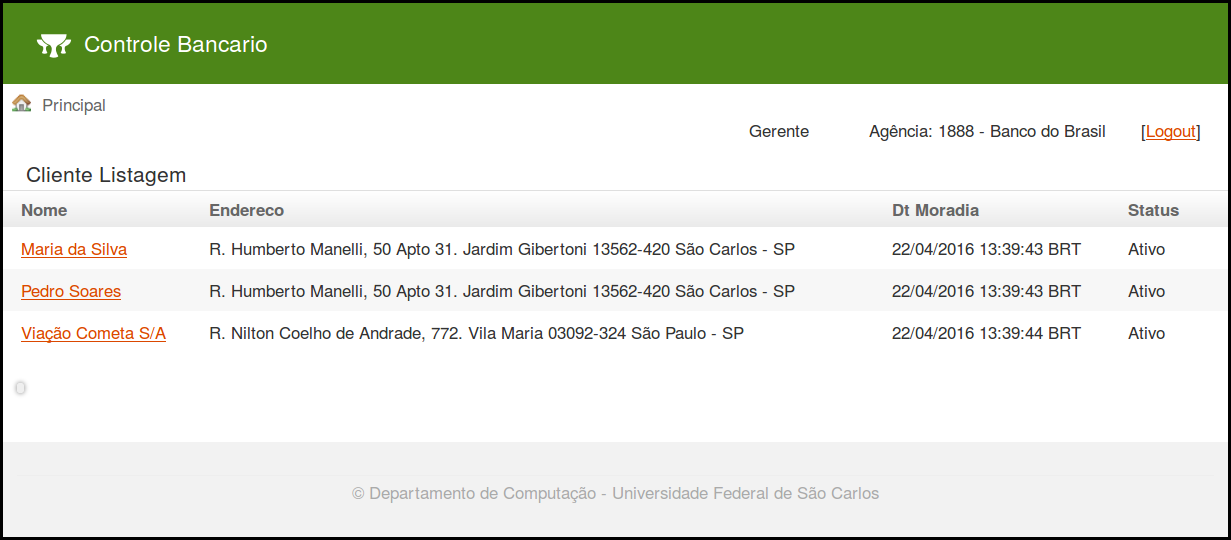
\includegraphics[width=14cm]{indexCliente}
\caption{Lista de clientes}
\label{indexClienteFig}
\end{figure}

\vspace{0.4cm}

\begin{itemize}

\item   {\bf   ContaCliente}   caso   deseje  acessar/atualizar   a   lista   de
  relacionamentos entre clientes e contas da agência do usuário {\it logado};

\vspace{0.4cm}

\item  {\bf  Conta},  {\bf  ContaCorrente}  e {\bf  ContaPoupança}  caso  deseje
  acessar/atualizar  a lista  de  contas  da agência  do  usuário {\it  logado}.
  Figura~\ref{indexContaFig} apresenta  a lista de contas da  agência do usuário
  {\it logado}.  

\end{itemize}

\vspace{0.4cm}

\begin{itemize}

\begin{figure}[htbp]
\centering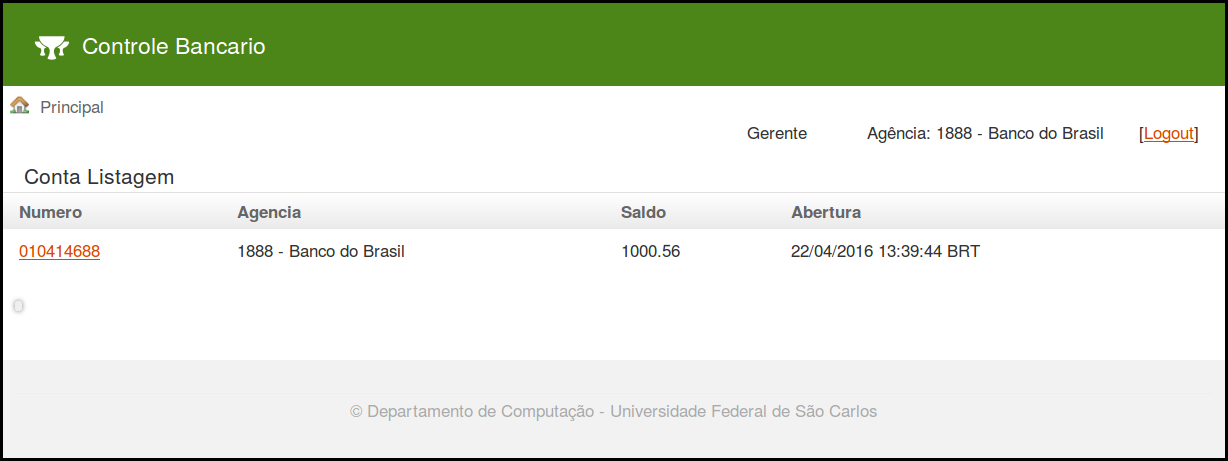
\includegraphics[width=14cm]{indexConta}
\caption{Lista de contas da agência do usuário {\it logado}}
\label{indexContaFig}
\end{figure}

\vspace{0.4cm}

\item  {\bf  Endereco}  caso  deseje  acessar/atualizar  a  lista  de  endereços
  cadastrados.
 
\end{itemize}

\newpage

\section{Preenchimento automático de endereços}\label{secAutoFill}

\vspace{0.5cm}

Essa seção  tem como objetivo  incorporar, na aplicação  {\bf ControleBancario},
algumas funcionalidades AJAX  relacionadas ao acesso a um  serviço {\it web}. Em
especial,   essa  seção   apresenta   a  implementação   da  funcionalidade   de
preenchimento automático dos atributos da classe de domínio {\bf Endereco}. 

\vspace{0.2cm}

Ou seja, dado o atributo CEP,  os demais atributos desse classe de domínio serão
preenchidos automaticamente.  Para prover  essa funcionalidade, será acessado um
serviço {\it web} que, dado um CEP como parâmetro, retorna as demais informações
de um endereço (logradouro, bairro, cidade, etc).  

\subsection{Template endereco/\_address.gsp}

\vspace{0.5cm}

O primeiro passo na  implementação da funcionalidade de preenchimento automático
de endereços  consiste em definir o {\it  template} {\bf endereco/\_address.gsp}
conforme  apresentado no  Código~\ref{codTemplateAddress}.  Esse {\it  template}
será utilizado pelas visões {\bf create.gsp}  e {\bf edit.gsp} e contém todos os
campos (exceto  o campo  CEP discutido a  seguir nessa seção)  responsáveis pela
entrada dos valores dos atributos da classe de domínio {\bf Endereco}.  

\begin{lstlisting}[caption={\it Template} {\bf endereco/\_address.gsp}, frame=trBL,
    float=htbp, label=codTemplateAddress] 
<%@ page import="br.ufscar.dc.dsw.Endereco" %>

<div class="fieldcontain ${hasErrors(bean: endereco, field: 'logradouro', 'error')}">
    <label for="logradouro">
        <g:message code="endereco.logradouro.label" default="Logradouro" />
    </label>
    <g:textField name="logradouro" maxlength="30" value="${endereco?.logradouro}"/>
</div>

<div class="fieldcontain ${hasErrors(bean: endereco, field: 'numero', 'error')}">
    <label for="numero">
        <g:message code="endereco.numero.label" default="Numero" />
    </label>
    <g:field name="numero" type="number" min="0" value="${endereco.numero}"/>
</div>

<div class="fieldcontain ${hasErrors(bean: endereco, field: 'complemento', 'error')} ">
    <label for="complemento">
        <g:message code="endereco.complemento.label" default="Complemento" />

    </label>
    <g:textField name="complemento" maxlength="20" value="${endereco?.complemento}"/>
</div>

<div class="fieldcontain ${hasErrors(bean: endereco, field: 'bairro', 'error')} ">
    <label for="bairro">
        <g:message code="endereco.bairro.label" default="Bairro" />
    </label>
    <g:textField name="bairro" maxlength="20" value="${endereco?.bairro}"/>
</div>

<div class="fieldcontain ${hasErrors(bean: endereco, field: 'cidade', 'error')} ">
    <label for="cidade">
        <g:message code="endereco.cidade.label" default="Cidade" />
    </label>
    <g:select id="cidade" name="cidade.id" from="${br.ufscar.dc.dsw.Cidade.list()}" optionKey="id" 
                          value="${endereco?.cidade?.id}" class="many-to-one"/>
</div>
\end{lstlisting}

Código~\ref{codEnderecoCreate}   mostra   a   reimplementação  da   visão   {\bf
  endereco/create.gsp}. Por  questão de brevidade, apenas  serão apresentadas as
mudanças realizadas  nessa visão.   Pode-se observar que  o {\it  template} {\bf
  \_address.gsp}  é  renderizado  (linha  15)  no contexto  do  formulário  HTML
definido pela {\it tag} {\bf g:form}. 

\newpage

No contexto  do formulário  foi definido  também, o campo  de texto  CEP (linhas
22-24)   de   tal  forma   que   o   tratamento   ao  evento   Javascript   {\it
  onblur}\footnote{O evento {\it onblur} ocorre  quando um objeto perde o foco.}
consiste em invocar, passando como parâmetro o conteúdo do campo de texto CEP, a
ação    {\bf   addressByCEP()}    do   controlador    {\bf   EnderecoController}
(Seção~\ref{secEnderecoController}).  

\begin{lstlisting}[caption={\bf endereco/create.gsp},
    frame=trBL, float=htbp, label=codEnderecoCreate, numbers=left]
<div id="create-endereco" class="content scaffold-create" role="main">
    <h1><g:message code="default.create.label" args="[entityName]" /></h1>
    <g:if test="${flash.message}">
       <div class="message" role="status">${flash.message}</div>
    </g:if>
    <g:hasErrors bean="${this.endereco}">
        <ul class="errors" role="alert">
            <g:eachError bean="${this.endereco}" var="error">
                <li <g:if test="${error in org.springframework.validation.FieldError}">
                                  data-field-id="${error.field}"</g:if>><g:message error="${error}"/></li>
            </g:eachError>
        </ul>
    </g:hasErrors>
    <g:form action="save">
       <fieldset class="form">

          <div class="fieldcontain ${hasErrors(bean: endereco, field: 'CEP', 'error')} required">
                <label for="CEP">
                    <g:message code="endereco.CEP.label" default="CEP" />
                    <span class="required-indicator">*</span>
                 </label>
                 <g:textField name="CEP" maxlength="9" required="" value="${endereco?.CEP}"
                           onblur="${remoteFunction(action: 'addressByCEP', update: [success: 'addressContainer'],
                                   params: '\'cep=\' + this.value', asynchronous: false)}"/>
           </div>

           <div id="addressContainer">
                <g:render template="address" bean="${endereco}"/>
           </div>

        </fieldset>
        <fieldset class="buttons">
             <g:submitButton name="create" class="save" 
                             value="${message(code: 'default.button.create.label', default: 'Create')}" />
        </fieldset>
    </g:form>
</div>
\end{lstlisting}

O  {\it template} {\bf  endereco/\_address.gsp} será  atualizado em  resposta ao
retorno  da   invocação  da  ação  {\bf  addressByCEP()}   do  controlador  {\bf
  EnderecoController}.   Ou  seja,  as  informações retornadas  pela  ação  {\bf
  addressByCEP()}  serão utilizados  para o  prenchimento automático  dos demais
atributos da classe de domínio {\bf Endereco}.  

\vspace{0.2cm}

É importante salientar que  o {\it template} {\bf endereco/\_address.gsp} apenas
será atualizado pois encontra-se no escopo  de uma {\it tag} {\bf div} cujo {\bf
  id} ({\it addressContainer}) é igual ao valor do atributo {\bf update/success}
de {\bf remoteFunction} (Código~\ref{codEnderecoCreate}, linhas 23 e 27). 

\vspace{0.2cm}

\begin{remark}
Análogo  à  visão {\bf  endereco/create.gsp},  a  visão {\bf  endereco/edit.gsp}
também   necessita  ser   alterada   para  utilizar   o   {\it  template}   {\bf
  \_address.gsp}.  Fica como exercício para o leitor realizar tal alteração. 
\end{remark}

\newpage

\subsection{Controlador: EnderecoController}
\index{Serviços {\it web} REST!Cliente}
\label{secEnderecoController}

\vspace{0.5cm}

O segundo  passo na implementação da funcionalidade  de preenchimento automático
de endereços consiste  em implementar a ação {\bf  addressByCEP()} que, conforme
discutido    anteriormente,    é    invocado    pelo   {\it    template}    {\bf
  endereco/\_address.gsp} (Código~\ref{codEnderecoController}). 

\vspace{0.2cm}

\hyphenation{addressByCEP}

Essa  ação   utiliza  as  funcionalidades   providas  pelo  {\it   plugin}  {\bf
  grails-datastore-rest-client} que  possibilita o  acesso a serviços  {\it web}
REST.  Ou seja, conforme pode-se observar, a ação {\bf addressByCEP~()} invoca um
serviço  {\it web}  REST que,  dado  um CEP  como parâmetro,  retorna as  demais
informações de um endereço (logradouro, bairro, cidade, etc).  

\vspace{0.2cm}

O  serviço {\it  web} REST  retorna  o endereço  em formato  JSON\footnote{JSON,
  acrônimo  para  {\it JavaScript  Object  Notation},  é  um formato  leve  para
  intercâmbio de dados computacionais.} com as seguintes informações: 

\vspace{0.3cm}

\begin{itemize}

\item {\bf uf} que armazena a sigla da unidade federativa/estado;

\vspace{0.3cm}

\item {\bf cidade} que armazena o nome da cidade;

\vspace{0.3cm}

\item {\bf bairro} que armazena o nome do bairro;

\vspace{0.3cm}

\item {\bf  tipo\_logradouro} que armazena  o tipo do logradouro  (rua, avenida,
  etc); e

\vspace{0.3cm}

\item {\bf logradouro} que armazena o nome do logradouro.

\end{itemize}

\begin{lstlisting}[caption=Controlador  {\bf EnderecoController}, frame  = trBL,
    float=htbp, label=codEnderecoController] 
class EnderecoController {

    // Demais a^çõ^es/atributos/m^é^todos do controlador EnderecoController

    def addressByCEP() {

        String restUrl="http://cep.republicavirtual.com.br/web_cep.php?cep="+params.cep+"&formato=json"

        RestBuilder rBuilder = new RestBuilder()
        RestResponse rResponse = rBuilder.get(restUrl)

        def html = rResponse?.json
        params.estado = Estado.findBySigla(html.uf)
        params.cidade = Cidade.findByNomeAndEstado(html.cidade, params.estado)
        params.bairro = html.bairro
        params.logradouro = html.tipo_logradouro + " " + html.logradouro

        render template: 'address', model: [endereco: new Endereco(params)]
    }
}
\end{lstlisting}

\vspace{0.3cm}

Tomando como base as informações retornadas  pelo serviço {\it web} REST, a ação
{\bf addressByCEP()}  cria uma instância da  classe de domínio  {\bf Endereco} e
retorna  essa   instância  para  ser   renderizada  pelo  {\it   template}  {\bf
  endereco/\_address.gsp}. 

\vspace{0.2cm}

Figura~\ref{figEnderecoCEP} apresenta a página de cadastro de um endereço (visão
{\bf endereco/create.gsp}) em que os  atributos {\bf logradouro}, {\bf bairro} e
{\bf cidade} foram preenchidos automaticamente pelas informações retornadas pela
ação {\bf addressByCEP()}.  

\vspace{0.3cm}

\begin{figure}[htbp]
\centering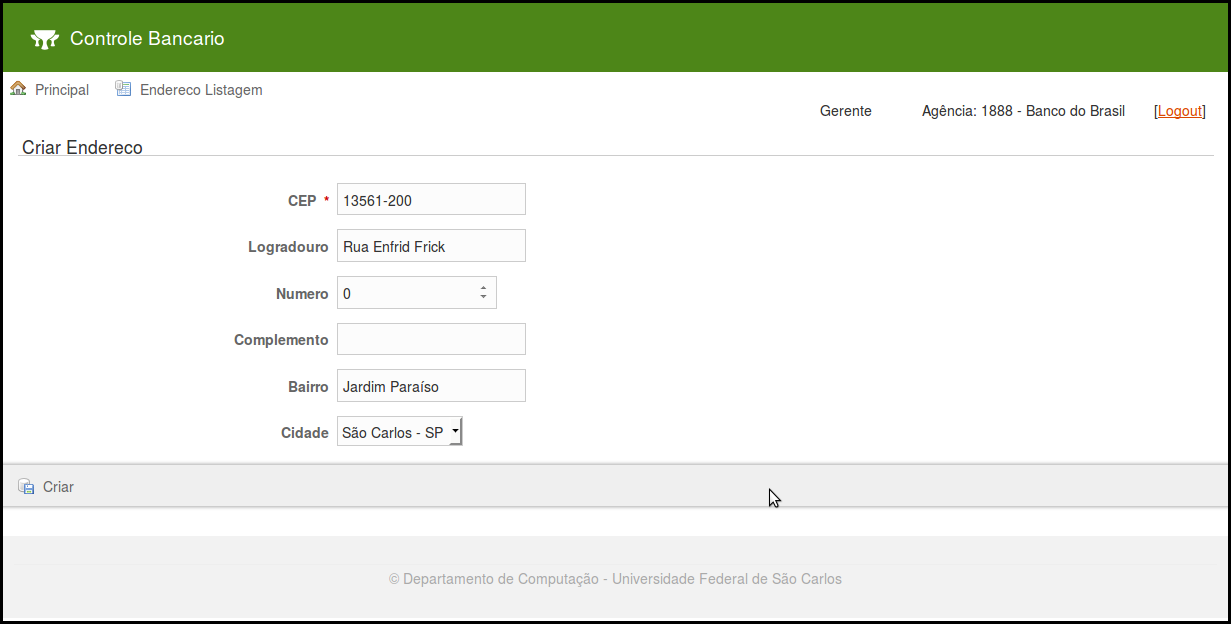
\includegraphics[width=14.5cm]{enderecoCEP}
\caption{Visão {\bf endereco/create.gsp}: Preenchimento automático de atributos}
\label{figEnderecoCEP}
\end{figure}

\newpage

\section{Considerações finais}

\vspace{0.3cm}

Esse capítulo  apresentou a terceira  versão da implementação da  aplicação {\bf
  ControleBancario}.         O        código-fonte        dessa        aplicação
({\footnotesize\texttt{ControleBancarioV3}})   encontra-se   disponível  em   um
repositório {\it GitHub}\footnote{URL: {\url{https://github.com/delanobeder/FG}}}.  

\vspace{0.2cm}

Dando  continuidade, o  próximo  capítulo  apresenta o  {\it  overview} de  mais
algumas  funcionalidades  presentes  em  Grails  que  não  foram  abordadas  nos
capítulos anteriores.  



%-------------------------------------------------------------------------------
%	CAPÍTULO 5
%-------------------------------------------------------------------------------

%\chapter{Controle Bancário: Versão 4}\label{interface}

Neste  capítulo,   dando  continuidade   ao  desenvolvimento  em   Grails,  será
apresentado o  processo de  desenvolvimento da quarta  versão da  aplicação {\bf
  ControleBancario}. Nessa versão são incorporadas as seguintes funcionalidades:

\begin{itemize}

\vspace{0.5cm}

\item Implementação  da funcionalidade de  visualização e impressão  de extratos
  bancários associados às  contas bancárias. Para tal, serão  utilizados os {\it
    plugins} {\bf wkhtmltopdf} e {\bf google-visualization};

\vspace{0.5cm}

\item  Implementação de  um serviço  {\it web}  REST que  retorna uma  lista (em
  formato JSON ou XML) de agências de um determinado banco; 

\end{itemize}

\section{Configuração da aplicação} 

\vspace{0.5cm}

\noindent{\bf   Instalação   de    {\it   plugins}.}    Na   implementação   das
funcionalidades da aplicação  {\bf ControleBancario}, discutidas nesse capítulo,
serão  utilizados os  {\it plugins}  Grails {\bf  richui}, {\bf  pure-css}, {\bf
  wkhtmltopdf} e  {\bf google-visualization}. Conforme  discutido anteriormente,
para  instalar   esses  {\it  plugins},  adicione  as   linhas,  descrevendo  as
dependências,  no  arquivo  {\bf  BuildConfig.groovy} conforme  apresentado  nas
linhas 54-57 do Código~\ref{codBuildConfig4}.  
\index{Plugins!richui}
\index{Plugins!pure-css}
\index{Plugins!wkhtmltopdf}
\index{Plugins!google-visualization}

\newpage

\begin{lstlisting}[numbers=left,  caption={\bf  BuildConfig.groovy}, frame=trBL,
    float=htbp, label=codBuildConfig4]
grails.project.dependency.resolution = {
    // inherit Grails' default dependencies
    inherits("global") {
        // specify dependency exclusions here; for example, uncomment this to disable ehcache:
        // excludes 'ehcache'
    }
    log "error" // log level of Ivy resolver, either 'error', 'warn', 'info', 'debug' or 'verbose'
    checksums true // Whether to verify checksums on resolve
    legacyResolve false // whether to do a secondary resolve on plugin installation, not advised and 
                        // here for backwards compatibility

    repositories {
        inherits true // Whether to inherit repository definitions from plugins

        grailsPlugins()
        grailsHome()
        mavenLocal()
        grailsCentral()
        mavenCentral()
        // uncomment these (or add new ones) to enable remote dependency resolution from public Maven repositories
        mavenRepo "http://repository.codehaus.org"
        //mavenRepo "http://download.java.net/maven/2/"
        //mavenRepo "http://repository.jboss.com/maven2/"
        mavenRepo "http://repo.spring.io/milestone/"
    }

    dependencies {
        // specify dependencies here under either 'build', 'compile', 'runtime', 'test' or 'provided' scopes e.g.
        // runtime 'mysql:mysql-connector-java:5.1.27'
        runtime 'org.postgresql:postgresql:9.3-1100-jdbc41'
    }

    plugins {
        // plugins for the build system only
        build ":tomcat:7.0.50"

        // plugins for the compile step
        compile ":scaffolding:2.0.1"
        compile ':cache:1.1.1'

        // plugins needed at runtime but not for compilation
        runtime ":hibernate:3.6.10.7" // or ":hibernate4:4.1.11.6"
        runtime ":database-migration:1.3.8"
        runtime ":jquery:1.10.2.2"
        runtime ":resources:1.2.1"
        // Uncomment these (or add new ones) to enable additional resources capabilities
        //runtime ":zipped-resources:1.0.1"
        //runtime ":cached-resources:1.1"
        //runtime ":yui-minify-resources:0.1.5"
        
        compile ":br-validation:0.3"
        compile ":spring-security-core:2.0-RC2"
        compile ":rest:0.8"
        compile ":richui:0.8"
        compile ":pure-css:0.4.2"
        compile ":wkhtmltopdf:0.1.7"
        compile ":google-visualization:0.7"
    }
}
\end{lstlisting}

\noindent{\bf Instalação  do wkhtmltopdf.} Na versão,  discutida nesse capítulo,
extratos bancários, associados às contas bancárias, poderão ser convertidos para
o formato pdf.  Para tal, será necessária a instalação do {\bf wkhtmltopdf}, que
consiste em uma ferramenta {\it open-source} que converte arquivos {\bf html} em
arquivos {\bf pdf}. 

A instalação no  sistema operacional linux Ubuntu pode  ser realizada através do
comando  {\bf sudo  apt-get  install wkhtmltopdf  -q},  conforme apresentada  na
Figura~\ref{figWkhtmltopdf}.  

\vspace{0.5cm}

\begin{remark}
Para  os demais  sistemas operacionais,  sugere-se  ao leitor  que verifique  as
instruções           de           instalação           disponíveis           em:
{\footnotesize\url{http://wkhtmltopdf.org}}.  
\end{remark}

\begin{figure}[htbp]
\centering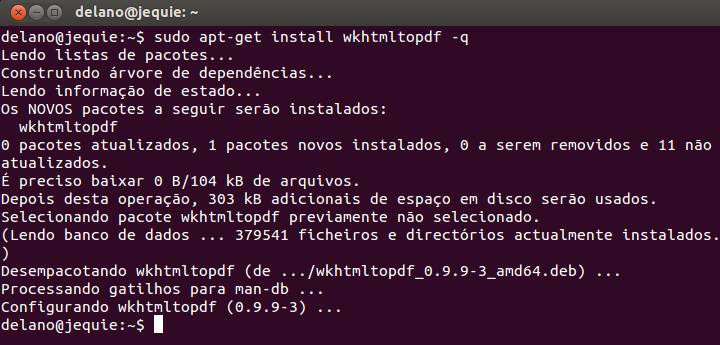
\includegraphics[width=12cm]{wkhtmltopdf}
\caption{Instalação do {\bf wkhtmltopdf}}
\label{figWkhtmltopdf}
\end{figure}

\newpage

\noindent{\bf  Configuração  de {\it  plugins}.}   Após  a  instalação dos  {\it
  plugins}  é   necessário  incluir   algumas  configurações  no   arquivo  {\bf
  conf/Config.groovy} (Código~\ref{codConfig}). Por questão de brevidade, apenas
serão apresentadas as mudanças realizadas nesse arquivo.  

\begin{itemize}

\vspace{0.3cm}

\item O primeiro bloco adiciona o  formato {\bf pdf} na lista de {\it MimeTypes}
  manipulados pela aplicação;

\vspace{0.3cm}

\item O segundo bloco configura a maneira em que os {\it scriptlets} (trechos de
  código)  são tratadas  nas  visões. Essa  alteração  é necessária  para o  bom
  funcionamento da geração de arquivos {\bf pdf};

\vspace{0.3cm}

\item Por fim,  o terceiro bloco indica onde  encontra-se instalada a ferramenta
  {\bf wkhtmltopdf}. 

\end{itemize}

\begin{lstlisting}[caption={\bf    Config.groovy},    frame=trBL,    float=htbp,
    label=codConfig]

grails.mime.types = [ // the first one is the default format
    all:           '*/*', // 'all' maps to '*' or the first available format in withFormat
    atom:          'application/atom+xml',
    css:           'text/css',
    csv:           'text/csv',
    pdf:           'application/x-pdf',
    form:          'application/x-www-form-urlencoded',
    html:          ['text/html','application/xhtml+xml'],
    js:            'text/javascript',
    json:          ['application/json', 'text/json'],
    multipartForm: 'multipart/form-data',
    rss:           'application/rss+xml',
    text:          'text/plain',
    hal:           ['application/hal+json','application/hal+xml'],
    xml:           ['text/xml', 'application/xml']
]

grails {
    views {
        gsp {
            encoding = 'UTF-8'
            htmlcodec = 'xml' // use xml escaping instead of HTML4 escaping
            codecs {
                expression = 'html' // escapes values inside ${}
                scriptlet = 'none' // escapes output from scriptlets in GSPs
                taglib = 'none' // escapes output from taglibs
                staticparts = 'none' // escapes output from static template parts
            }
        }
        // escapes all not-encoded output at final stage of outputting
        filteringCodecForContentType {
            //'text/html' = 'html'
        }
    }
}
 
grails.plugin.wkhtmltox.binary = "/usr/bin/wkhtmltopdf"
\end{lstlisting}

\section{Extratos Bancários}

\vspace{0.5cm}

O  controlador  {\bf ExtratoController}  é  responsávela  pela implementação  da
funcionalidade de  visualização e impressão de extratos  bancários associados às
contas bancárias.  A implementação desse controlador  encontra-se apresentada no
Código~\ref{codExtratoController}. 

\begin{lstlisting}[caption=  Controlador  {\bf  ExtratoController},  frame=trBL,
    float=htbp, label=codExtratoController, numbers=left] 
package br.ufscar.dc.dsw
import java.text.SimpleDateFormat
import org.springframework.security.access.annotation.Secured

@Secured('ROLE_CLIENTE')
class ExtratoController { 

    def index() {
        def linhas = getLinhas()
        if(params?.format && params.format == "pdf"){
            render( filename:"extrato.pdf",
                view:"/extrato/_pdf",
                model:[lines: linhas, contaCliente:session.contaCliente],
                marginLeft:20,
                marginTop:35,
                marginBottom:20,
                marginRight:20,
                headerSpacing:10,
            )   
        }
        model:[lines: linhas]
    }
    
    def chart = {
        def columns = [['date', 'Dia'], ['number', 'Saldo (R$)']]
        def lines = []
        def linhas = getLinhas()
        def anterior = null
        SimpleDateFormat formato = new SimpleDateFormat("dd/MM/yyyy")

        linhas.reverse().each {
            def atual = formato.format(it.data)
            if (!atual.equals(anterior)) {
                lines.add([it.data, it.saldo])                
            }
            anterior = it.data
        }
          
        ["columns": columns, "lines": lines]
    }

    private List<Line> getLinhas() {
        def conta = Conta.get(session.contaCliente.conta.id)
        def saldo = conta.saldo
        def results = Transacao.findAllByContaCliente(session.contaCliente, [sort:"data"])
        results.each {
            saldo -= it.getValorReal()
        }

        List<Line> linhas = new ArrayList<Line>();
        Line linha = new Line(session.contaCliente.conta.abertura, "ABERTURA", saldo)
        linhas.add(linha)       

        results.each {
            saldo += it.getValorReal()
            linha = new Line(it.data, it.tipo, saldo, it.valor, it.motivo)
            linhas.add(linha)
        }

        linha = new Line(new Date(), "SALDO ATUAL", saldo)
        linhas.add(linha)
        return linhas
    }
}
\end{lstlisting} 

\vspace{0.5cm}

\begin{itemize}

\item A  ação {\bf index()}  (linhas 7-21) simplesmente invoca  implicitamente a
  visão {\bf  index.gsp} (Código~\ref{codExtratoIndex}) que  representa extratos
  bancários em formato HTML.   Adicionalmente, essa ação renderiza, utilizando o
  {\it plugin}  {\bf wkhtmltopdf}, o  arquivo {\bf extrato.pdf} baseado  no {\it
    template}  {\bf extrato/\_pdf.gsp} (Código~\ref{codPdfTemplate}).   Ou seja,
  essa ação é também responsável  por gerar os arquivos que representam extratos
  bancários em formato PDF; 

\vspace{0.5cm}

\item A ação  {\bf chart()} (linhas 23-38) simplesmente  invoca implicitamente a
  visão   {\bf  chart.gsp}   (Código~\ref{codChart})  que   será   discutida  na
  Seção~\ref{secExtratoVisoes};

\vspace{0.5cm} 

\item  É importante salientar  que as  ações (e  respectivas visões)  utilizam o
  método  privado  {\bf  getLinhas()}   (linhas  40-58)  retorna  uma  lista  de
  instâncias  da classe  {\bf  Line}.   Conforme pode-se  observar,  a lista  de
  instâncias da classe  {\bf Line} é construída através da  iteração da lista de
  transações (ordenadas pela data) associadas às contas bancárias; 

\vspace{0.5cm}

\item      A     classe      Java     {\bf      Line}\footnote{Arquivo:     {\bf
    src/br/ufscar/dc/dsw/Line.java}}    (Código~\ref{codLine})    armazena    as
  informações (atributos:  {\bf data}, {\bf  tipo}, {\bf motivo}, {\bf  valor} e
  {\bf saldo})  relacionadas às  transações e representa  cada linha  do extrato
  bancário a ser visualizado e/ou impresso.  

\end{itemize}

\vspace{0.5cm}

\begin{lstlisting}[caption=Classe  Java   {\bf  Line},  frame=trBL,  float=htbp,
    label=codLine] 
package br.ufscar.dc.dsw;

import java.util.Date;

public class Line implements Comparable<Line>{
    
    private final Date data;
    
    private final String tipo;
    
    private final String motivo;
    
    private final Double valor;
    
    private final Double saldo;

    public Line(Date data, String tipo, Double saldo, Double valor, String motivo) {
        this.data = data;
        this.tipo = tipo;
        this.saldo = saldo;
        this.valor = valor;
        this.motivo = motivo;
    }
    
    public Line(Date data, String tipo, double saldo) {
        this(data, tipo, saldo, null, null);
    }
    

    public Date getData() {
        return data;
    }

    public String getTipo() {
        return tipo;
    }

    public String getMotivo() {
        return motivo;
    }

    public Double getValor() {
        return valor;
    }

    public Double getSaldo() {
        return saldo;
    }    

    
    @Override
    public int compareTo(Line o) {
        return this.data.compareTo(o.data);
    }

    @Override
    public String toString() {
        return data.toString() + " - " + valor + " - " + saldo;
    }
    
}
\end{lstlisting}

\newpage

\subsection{Visões}\label{secExtratoVisoes}

\vspace{0.5cm}

Relembrando   a   discussão  da   Seção~\ref{secEstatico},   para  cada   método
correspondente a  uma ação em um  controlador é criada  uma correspondente visão
(arquivo  com  extensão {\bf  .gsp}).   Assim, a  ação  {\bf  index()}, de  {\bf
  ExtratoController},  tem  o  correspondente  {\bf  index.gsp}  que  representa
extratos  bancários em  formato HTML.  A implementação  dessa  visão encontra-se
apresentada no Código~\ref{codExtratoIndex}.

\vspace{0.3cm}

\noindent  Figura~\ref{figExtratoHTML}  apresenta   um  exemplo  de  um  extrato
bancário representado pela visão {\bf extrato/index.gsp}. É importante salientar
que essa visão  já apresenta um leiaute mais  responsivo: menu horizontal (linha
14) e tabela (linha 26). 

\vspace{0.2cm}

\begin{lstlisting}[caption=Visão {\bf extrato/index.gsp}, frame=trBL, float=htbp,
    label=codExtratoIndex, numbers=left]
<%@ page import="org.grails.plugins.google.visualization.data.Cell; 
                 org.grails.plugins.google.visualization.util.DateUtil" %>
<%@ page import="br.ufscar.dc.dsw.Transacao" %>
<!DOCTYPE html>
<html>
  <head>
    <meta name="layout" content="main">
    <title><g:message code="extrato.statement"/></title>
    <r:require module="pure-all" />
  </head>
  <body>
    <a href="#list-transacao" class="skip" tabindex="-1">
    <g:message code="default.link.skip.label" default="Skip to content&hellip;"/></a>
    <div class="pure-menu pure-menu-open pure-menu-horizontal">
      <ul>
        <li><a class="home" href="${createLink(uri: '/')}"><g:message code="default.home.label"/></a></li>
        <li><g:link action="chart"><g:message code="extrato.chart" default="Chart" /></g:link></li>
        <li><g:link controller="logout">Logout</g:link></li>
      </ul>
    </div>
    <div id="list-transacao" class="content scaffold-list" role="main">
      <h1><g:message code="extrato.statement"/></h1>
      <g:if test="${flash.message}">
        <div class="message" role="status">${flash.message}</div>
      </g:if>
      <table class="pure-table pure-table-bordered">
        <thead>
          <tr>
            <th><g:message code="transacao.data"/></th>
            <th><g:message code="transacao.tipo"/></th>
            <th><g:message code="transacao.motivo"/></th>
            <th><g:message code="extrato.valor"/></th>
            <th><g:message code="extrato.saldo"/></th>
          </tr>
        </thead>
        <tbody>
          <g:each in="${lines}" status="i" var="linha">
            <tr class="${(i % 2) == 0 ? 'even' : 'odd'}">
             <td><g:formatDate date="${linha.data}" type="date" style="SHORT"/></td>
             <td>${fieldValue(bean: linha, field: "tipo")}</td>
             <td>${fieldValue(bean: linha, field: "motivo")}</td>
             <td><g:formatNumber number="${linha.valor}" type="currency" /></td>
             <td><g:formatNumber number="${linha.saldo}" type="currency" /></td>
            </tr>
          </g:each>
        </tbody>
      </table>
      <center>
        <h4>
          <g:message code="extrato.saveaspdf"/>
          <g:link action="index.pdf">
            <img src="${resource(dir: 'images', file: 'pdf.jpg')}" alt="PDF" width="18px"/>
          </g:link>
        </h4>
      </center>
    </div>
  </body>
</html>
\end{lstlisting}

\vspace{0.2cm}

\noindent Em  complemento, essa visão adiciona  um {\it link}  (linha 51-53) que
possibilita salvar o extrato em  formato PDF. Conforme pode-se observar que esse
{\it  link} invoca  a ação  {\bf index}  do controlador  {\bf ExtratoController}
passando o parâmetro {\bf format} com o  valor igual a {\bf pdf}.  Nesse caso, o
controlador {\bf  ExtratoController} renderiza,  utilizando o {\it  plugin} {\bf
  wkhtmltopdf},  o arquivo  {\bf  extrato.pdf} baseado  no  {\it template}  {\bf
  extrato/\_pdf.gsp}.

\begin{figure}[htbp]
\centering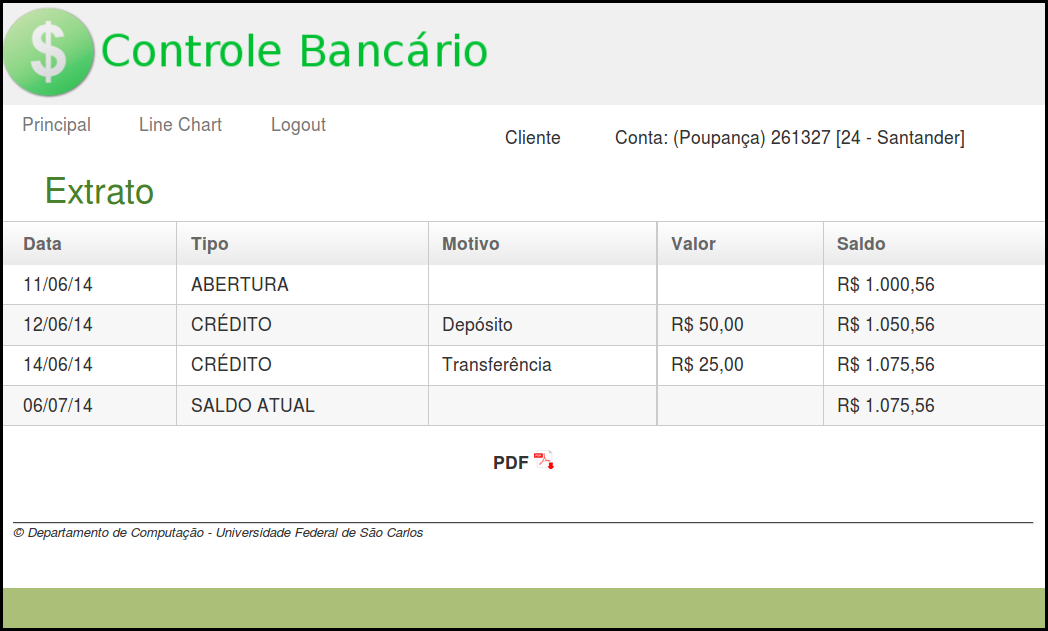
\includegraphics[width=12cm]{extrato}
\caption{Extrato Bancário em formato HTML}
\label{figExtratoHTML}
\end{figure}

Conforme   pode-se   observar,   o   {\it  template}   {\bf   extrato/\_pdf.gsp}
(Código~\ref{codPdfTemplate}) define  uma página HTML que será  convertida em um
arquivo  PDF.  Figura~\ref{figExtratoPDF}  apresenta  um exemplo  de um  extrato
bancário, em formato PDF, gerado pela ação {\bf index()}.

\begin{figure}[h]
\centering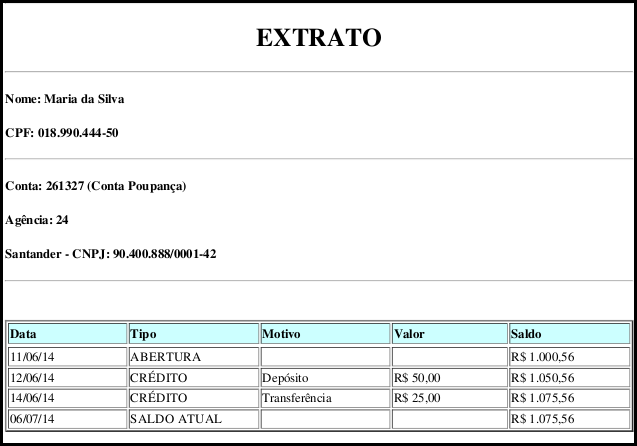
\includegraphics[width=11cm]{extratoPDF}
\caption{Extrato Bancário em formato PDF}
\label{figExtratoPDF}
\end{figure}

\newpage

\begin{lstlisting}[caption={\it Template} {\bf extrato/\_pdf.gsp}, frame=trBL,
    label=codPdfTemplate]
<%@ page import="br.ufscar.dc.dsw.ContaCorrente" %>
<%@ page import="br.ufscar.dc.dsw.ClienteFisico" %>
<hr/>
<center>
  <h1>EXTRATO</h1>
</center>
<hr/>
<h4>Nome: ${contaCliente.cliente.nome}</h4>
<h4>
  ${contaCliente.cliente instanceof ClienteFisico ? "CPF: " + contaCliente.cliente.CPF : 
                                                    "CNPJ: " + contaCliente.cliente.CNPJ}
</h4>
<hr/>
<h4>Conta: ${contaCliente.conta.numero}
  (${contaCliente.conta instanceof ContaCorrente ? "Conta Corrente" : "Conta Poupan^ç^a"})</h4>
<h4>Ag^ê^ncia: ${contaCliente.conta.agencia.numero}</h4>
<h4>${contaCliente.conta.agencia.banco} - CNPJ: ${contaCliente.conta.agencia.banco.CNPJ}</h4>
<hr/>
<br/>
<br/>
<table style="text-align: left; margin-left: auto; margin-right: auto;" class="pure-table pure-table-bordered" 
       border="2">
  <thead> 
    <tr>
      <th style="width: 200px; background-color: rgb(204, 255, 255);">Data</th>
      <th style="width: 200px; background-color: rgb(204, 255, 255);">Tipo</th>
      <th style="width: 200px; background-color: rgb(204, 255, 255);">Motivo</th>
      <th style="width: 200px; background-color: rgb(204, 255, 255);">Valor</th>
      <th style="width: 200px; background-color: rgb(204, 255, 255);">Saldo</th>
    </tr>
   </thead> 
   <tbody>
     <g:each in="${lines}" status="i" var="linha"> 
       <tr class="${(i % 2) == 0 ? 'even' : 'odd'}">
         <td><g:formatDate date="${linha.data}" type="date"/></td>
         <td>${fieldValue(bean: linha, field: "tipo")}</td>
         <td>${fieldValue(bean: linha, field: "motivo")}</td>
         <td><g:formatNumber number="${linha.valor}" type="currency"/></td>
         <td><g:formatNumber number="${linha.saldo}" type="currency"/></td>
       </tr>
     </g:each>
   </tbody>
</table>
<br/>
<br/>
<hr/>
<center>
  <h6>&copy; Departamento de Computa^çã^o - Universidade Federal de S^ã^o Carlos</h6>
  <h6><g:formatDate date="${new Date()}" type="datetime" style="LONG"/></h6>
</center>
\end{lstlisting}

A  visão  {\bf extrato/chart.gsp}  renderiza,  utilizando  o  {\it plugin}  {\bf
  google-visualization},  um gráfico  de  linhas que  representa a  movimentação
financeira  das  contas  bancárias.  A  implementação  dessa  visão  encontra-se
apresentada no Código~\ref{codChart}.  

\vspace{0.3cm}

\noindent  Conforme  pode-se  observar  essa  visão utiliza  a  {\it  tag}  {\bf
  <gvisualization:lineCoreChart>} para gerar um gráfico de linhas com os valores
({\bf columns} e {\bf lines}) retornados pela ação {\bf chart()}.  

\vspace{0.4cm}

\begin{lstlisting}[caption=Visão {\bf extrato/chart.gsp}, frame=trBL,
    label=codChart]
<%@ page import="org.grails.plugins.google.visualization.data.Cell; 
                 org.grails.plugins.google.visualization.util.DateUtil" %>
<html>
  <head>
    <title>Movimenta^çã^o Financeira</title>
    <meta name="layout" content="main" />
    <gvisualization:apiImport/>
    <r:require module="pure-all" />
  </head>
  <body>
    <div class="pure-menu pure-menu-open pure-menu-horizontal">
      <ul>
        <li><a class="home" href="${createLink(uri: '/')}"><g:message code="default.home.label"/></a></li>
        <li><g:link controller="extrato"><g:message code="extrato.statement"/></g:link></li>
        <li><g:link controller="logout">Logout</g:link></li>
      </ul>
    </div>
    <div id="list-transacao" class="content scaffold-list" role="main">
       <div id="linechart"></div>
       <gvisualization:lineCoreChart elementId="linechart" width="${800}" height="${300}" 
                      title="Movimenta^çã^o Financeira" columns="${columns}" data="${lines}" />
    </div>
  </body>
</html>
\end{lstlisting}

\newpage

\noindent   Figura~\ref{figLineChart}  apresenta  um   exemplo  de   um  gráfico
renderizado  pela ação  {\bf chart.gsp}.   Esse gráfico  ilustra  a movimentação
financeira (créditos e débitos) de uma conta bancária.

\vspace{0.3cm}

\begin{figure}[h]
\centering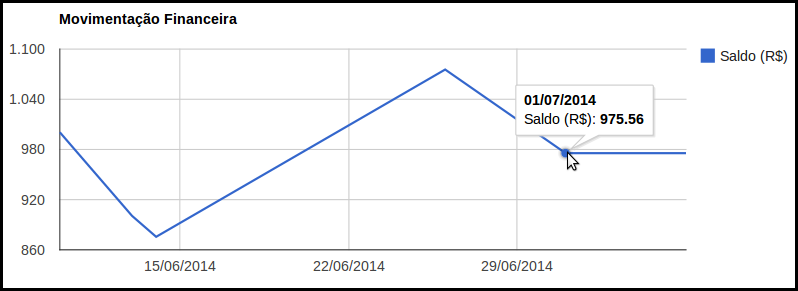
\includegraphics[width=14cm]{lineChart}
\caption{Movimentação financeira das contas bancárias}
\label{figLineChart}
\end{figure}

\section{Internacionalização - Mensagens I18n}
\index{Internacionalização~-~I18n}

\vspace{0.5cm}

Conforme pode-se observar pelas visões apresentadas/discutidas nesse capítulo, a
{\it tag} {\bf <g:message>} é utilizada para inserir rótulos internacionalizados
nessas  visões.  Dessa  forma, é  necessário adicionar  uma tradução,  para cada
idioma desejado, desses rótulos nos arquivos presentes no diretório {\bf i18n}. 

\vspace{0.2cm}

\noindent  Figura~\ref{figI18n} apresenta  a tradução  desses rótulos  que foram
inseridos  no arquivo  {\bf messages\_pt\_BR.properties}  ({\it  Message Bundle}
para o Português do Brasil).  

\vspace{0.3cm}

\begin{figure}[htbp]
\begin{mdframed}
\begin{footnotesize}
\begin{verbatim}
# Visão cliente/index.gsp
search.label=Busca de Cliente

# Visão main/index.gsp
main.options = Opções

# Visões - Controlador Transacao
transacao.main  = Conta Cliente & Caixa Eletrônico
transacao.value = Valor
transacao.data = Data
transacao.quem = Quem
transacao.motivo = Motivo
transacao.tipo = Tipo

# Visões - Controlador Extrato
extrato.statement = Extrato
extrato.chart = Line Chart
extrato.valor = Valor
extrato.saldo = Saldo
extrato.saveaspdf = PDF
\end{verbatim}
\end{footnotesize}
\end{mdframed}
\caption{Mensagens internacionalizadas}
\label{figI18n}
\end{figure}

\newpage

\section{Serviço {\it web} REST}\label{secWebREST}
\index{Serviços {\it web} REST}

\vspace{0.5cm}

REST  não é  uma tecnologia  em si,  pode ser  considerada mais  como  um padrão
arquitetural. O padrão arquitetural REST é  muito simples e envolve apenas o uso
simples de  XML ou  JSON como meio  de comunicação,  em conjunto com  padrões na
definição de  URLs que são  ``representações'' do sistema subjacente,  e métodos
HTTP, como GET, PUT,  POST e DELETE. Cada método HTTP é  mapeado para um tipo de
ação  do controlador.  Por exemplo,  o método  GET é  mapeado para  operações de
recuperação, o método  PUT é mapeado para operações de criação,  o método POST é
mapeado para operações de atualização e  assim por diante. Neste sentido REST se
encaixa muito bem com as operações CRUD. 

\vspace{0.2cm}

\noindent Essa seção  descreve a implementação de um serviço  {\it web} REST que
retorna uma lista  (em formato JSON ou XML) de agências  de um determinado banco
(parâmetro {\bf numero}). O controlador {\bf AgenciaController} é a escolha mais
óbvia para ser o responsável  por prover essa nova funcionalidade.  Dessa forma,
Código~\ref{codAgenciaController2}  apresenta  a   implementação  da  ação  {\bf
  list()},   do   controlador    {\bf   AgenciaController},   responsável   pela
implementação do serviço {\it web}  REST. Por questão de brevidade, apenas serão
apresentadas as mudanças realizadas nesse controlador.

\vspace{0.5cm}

\begin{lstlisting}[caption=Controlador  {\bf AgenciaController},  frame  = trBL,
    float=htbp, label=codAgenciaController2] 
import grails.converters.JSON
import grails.converters.XML

// Demais imports do controlador AgenciaController

class AgenciaController { 

    // Demais a^çõ^es/atributos/m^é^todos do controlador AgenciaController
   
    @Secured('IS_AUTHENTICATED_ANONYMOUSLY')
    def list() {
        
        def banco = Banco.findAllByNumero(params.numero)
        def agencias = Agencia.findAllByBanco(banco)
        def estado = Estado.findBySigla(params.estado)
        def cidade = Cidade.findByNomeAndEstado(params.cidade, estado)
        
        List<Info> lista = new ArrayList<Info>()
        
        agencias.each {
            
            if (!params.cidade || it.endereco.cidade == cidade) {
                Info info = new Info(it.banco.nome, it.numero, 
                    it.nome, it.endereco.toString())
            
                lista.add(info)
            }
        }
            
        withFormat {
            json { render lista as JSON }
            xml { render lista as XML }
        }
    }
}
\end{lstlisting}

\begin{itemize}

\vspace{0.5cm}

\item  A anotação  {\bf  @Secured('IS\_AUTHENTICATED\_ANONYMOUSLY')} indica  que
  esse serviço {\it web} é público e pode ser acessado por qualquer usuário e/ou
  aplicação.  

\vspace{0.5cm} 

\item  É importante  salientar que  a  ação {\bf  list()} retorna  uma lista  de
  instâncias  da classe  {\bf  Info}.   Conforme pode-se  observar,  a lista  de
  instâncias da classe  {\bf Info} é construída através da  iteração da lista de
  agências    associadas    a    um    determinado   banco    (parâmetro    {\bf
    numero}).   Opcionalmente,  a ação  {\bf  list()}  pode  filtrar essa  lista
  visando  apenas  retornar  as  agências  situadas em  uma  determinada  cidade
  (parâmetros {\bf cidade} e {\bf estado}); 

\vspace{0.5cm}

\item      A     classe      Java     {\bf      Info}\footnote{Arquivo:     {\bf
    src/br/ufscar/dc/dsw/Info.java}}    (Código~\ref{codInfo})    armazena    as
  informações  (atributos:  {\bf numero},  {\bf  nome},  {\bf  endereco} e  {\bf
    banco}) relacionadas às agências bancárias.  

\vspace{0.5cm}

\item Por  fim, a ação {\bf  list()} constrói a  saída ao renderizar a  lista de
  instâncias da classe {\bf Info} (em formato JSON ou XML).  A conversão para os
  formatos JSON ou XML é realizada  através da utilização das classes {\bf JSON}
  e {\bf XML} do pacote {\bf grails.converters}. 

\end{itemize}

\begin{lstlisting}[caption=Classe  Java   {\bf  Info},  frame=trBL,  float=htbp,
    label=codInfo] 
package br.ufscar.dc.dsw;

public class Info {
    
    private final int numero;

    private final String nome;

    private final String endereco;

    private final String banco;

    public Info(String banco, int numero, String nome, String endereco) {
        this.banco = banco;
        this.numero = numero;
        this.nome = nome;
        this.endereco = endereco;
    }

    public String getBanco() {
        return banco;
    }

    public String getEndereco() {
        return endereco;
    }

    public String getNome() {
        return nome;
    }

    public int getNumero() {
        return numero;
    }
    
    
}
\end{lstlisting}

Figura~\ref{figJSON} ilustra  o acesso  desse serviço {\it  web} através  da URL
{\footnotesize\url{http://localhost:8080/ControleBancarioV4/agencia/list.json?numero=1}}.
É importante salientar  que essa URL define a ação a  ser acessada: {\bf list()}
do controlador {\bf AgenciaController}.  Adicionalmente, essa URL define o valor
do parâmetro {\bf numero} e o formato da resposta (formato JSON).

\vspace{0.5cm}

\begin{figure}[h]
\centering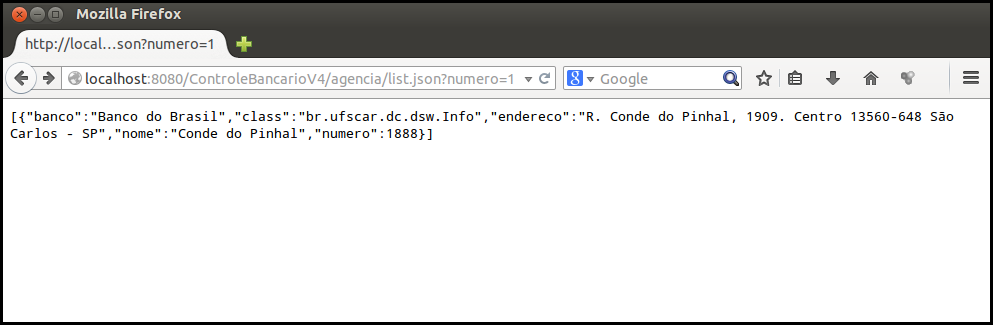
\includegraphics[width=15cm]{restJSON}
\caption{Serviço {\it web} REST: Formato JSON}
\label{figJSON}
\end{figure}

Analogamente, Figura~\ref{figXML} ilustra o acesso desse serviço {\it web} através da URL
{\footnotesize\url{http://localhost:8080/ControleBancarioV4/agencia/list.xml?numero=1}}. 
Novamente  essa URL define  a ação  a ser  acessada, o  valor do  parâmetro {\bf
  numero} e o formato da resposta (formato XML). 

\vspace{0.5cm}

\begin{figure}[h]
\centering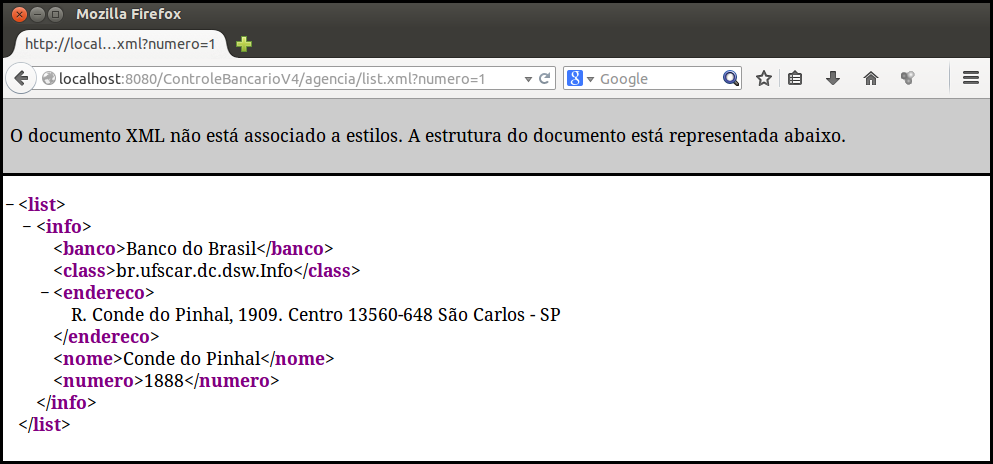
\includegraphics[width=15cm]{restXML}
\caption{Serviço {\it web} REST: Formato XML}
\label{figXML}
\end{figure}

\section{Considerações finais}

\vspace{0.3cm}


Esse  capítulo apresentou  a quarta  versão da  implementação da  aplicação {\bf
  ControleBancario}.         O        código-fonte        dessa        aplicação
({\footnotesize\texttt{ControleBancarioV4.zip}}) encontra-se  disponível no {\it
  Moodle}         do        curso,        localizado         no        endereço:
{\footnotesize\url{http://moodle.latosensu.dc.ufscar.br}}. Seguindo os passos do
tutorial   apresentado   obtem-se   esse   mesmo  código   da   aplicação   {\bf
  ControleBancario}.  




%-------------------------------------------------------------------------------
%	CAPÍTULO 5
%-------------------------------------------------------------------------------

\chapter{Considerações finais}\label{conclusoes}

Este  material  apresentou as  principais  funcionalidades  do framework  Grails
através da  descrição dos aspectos relacionados ao  desenvolvimento da aplicação
{\bf ControleBancario}.

\vspace{0.2cm}
\noindent Para finalizar esse material, esse capítulo apresenta o {\it overview}
de mais algumas funcionalidades presentes  em Grails que não foram abordadas nos
capítulos anteriores.

\section{Serviços Web}\index{Serviços Web}

\vspace{0.5cm}

Serviços web consistem  em fornecer uma API  web para a sua aplicação  web e são
geralmente implementados utilizando REST.

\subsection{REST}\index{Serviços Web!REST}

\vspace{0.5cm}

REST  não é  uma tecnologia  em si,  pode ser  considerada mais  como  um padrão
arquitetural. REST é muito simples e envolve apenas o uso simples de XML ou JSON
como meio de  comunicação, em conjunto com padrões na definição  de URLs que são
``representações'' do sistema subjacente, e  métodos HTTP, como GET, PUT, POST e
DELETE.

\vspace{0.2cm}

Cada método HTTP é  mapeado para um tipo de ação do  controlador. Por exemplo, o
método GET é mapeado para operações  de recuperação, o método PUT é mapeado para
operações de criação, o método POST é mapeado para operações de atualização e
assim por diante. Neste sentido REST  se encaixa muito bem com as operações CRUD
({\it Create}, {\it Read}, {\it Update} e {\it Delete}).

\vspace{0.2cm}

A abordagem mais fácil  para criar uma API REST em Grails  é expor uma classe de
domínio  como  um recurso  REST.   Isto  pode ser  feito  através  da adição  da
transformação   {\bf  grails.rest.Resource}   a  qualquer   classe   de  domínio
(Código~\ref{codREST}). 

\vspace{0.2cm}

Ao adicionar a transformação {\bf grails.rest.Resource} e especificar uma URI, a
classe de  domínio estará  automaticamente disponível como  um recurso  REST nos
formatos  XML ou  JSON.  Além  disso, a  transformação  registrará o  mapeamento
necessário   e    criará   um   controlador   (no   caso    do   exemplo,   {\bf
  LivroController}). Por  fim, é possível  alterar o padrão de  retorno (formato
JSON  ao  invés  do  formato  XML)  ao  definir  os  atributos  de  formatos  na
transformação {\bf grails.rest.Resource}.

\begin{lstlisting}[caption=Classe de domínio -- recurso REST, frame = trBL,
    float=htbp, label=codREST] 

import grails.rest.*

@Resource(uri='/livros', formats=['json', 'xml'])
class Livro {

    String titulo

    static constraints = {
        titulo blank:false
    }
}
\end{lstlisting}

Dessa forma, quando acessando a URL \url{http://localhost:8080/livros}, definida
no  atributo  {\bf  uri}   da  transformação  {\bf  grails.rest.Resource},  iria
renderizar uma resposta  para o acesso ao  recurso REST -- a lista  de livros no
formato JSON: 

\vspace{0.5cm}

\begin{cBox}
\begin{scriptsize}
\begin{verbatim}
[{"id":1,"titulo":"The Definitive Guide to Grails"},{"id":2,"titulo":"Grails in Action"}]
\end{verbatim}
\end{scriptsize}
\end{cBox}

\vspace{0.5cm}

Caso a  URL fosse \url{http://localhost:8080/livros.xml}, a resposta  seria -- a
lista de livros no formato XML:

\vspace{0.5cm}

\begin{cBox}
\begin{scriptsize}
\begin{verbatim}
<list>
  <livro id="1">
    <titulo>The Definitive Guide to Grails</titulo>
  </livro>
  <livro id="2">
    <titulo>Grails in Action</titulo>
  </livro>
</list>
\end{verbatim}
\end{scriptsize}
\end{cBox}

\vspace{0.5cm}

Para  maiores  informações  sobre   serviços  web  REST,  consulte  o  endereço:
{\footnotesize\url{https://grails.github.io/grails-doc/latest/guide/webServices.html}}.

\section{Automação de testes}

\vspace{0.5cm}

Essa seção apresenta algumas características de Grails que facilitam a automação
de  testes. Relembrando:  testes automatizados  te dão  segurança no  momento da
manutenção. No entanto, antes do início da discussão sobre tais características,
é fundamental relembrar  a diferença entre testes unitários  e de integração (ou
integrados). Para melhor explicar esses dois conceitos, utilizaremos a definição
presente no livro de Weissmann~\cite{wei15}: 

\vspace{0.2cm}

\begin{cBox}
{\it Grails nos  fornece por padrão dois tipos de  testes: unitário e integrado.
  O objetivo do teste unitário é  nos fornecer o ferramental necessário para que
  possamos verificar o  funcionamento de uma funcionalidade de  modo isolado, ou
  seja, sem que precisemos iniciar todo o sistema para isto.} 

\vspace{0.2cm}

{\it Isso nos  permite focar apenas na lógica  que estamos implementando naquele
  trecho do  sistema, mas por outro  lado, dado que  sempre precisamos interagir
  com outros  componentes arquiteturais, por exemplo, a  camada de persistência,
  um novo  problema surge. Como fazê-lo?  A resposta é  simples: criando versões
  falsas dos mesmos (os mocks). (...)}

\vspace{0.2cm}

{\it Testes unitários  nos fornecem, portanto, dependências do  nosso código que
  funcionam  em ``condições  ideais de  temperatura e  pressão'', ou  seja, elas
  funcionam exatamente  como gostaríamos,  o que pode  ser um problema,  mas nos
  ajuda a focar melhor naquilo que desejamos verificar.}

\vspace{0.2cm}
 
{\it Já testes integrados resolvem o problema da ``condição ideal de temperatura
  e pressão'' ao nos disponibilizar o sistema completo. Você não precisa mais de
  mocks, pois estará  usando o próprio sistema para  isso. São fundamentais para
  que vejamos  qual será  o comportamento do  sistema quando for  para produção,
  fornecendo-nos um ambiente que é o mais similar possível a este.}

\vspace{0.2cm}

\noindent ({WEISSMANN, H.~L. \emph{Falando  de Grails -- Altíssima produtividade
    no desenvolvimento web}. São Paulo: Casa do Código, 2015.)} 
\end{cBox}

\vspace{0.5cm}

Todos   os  testes   se  encontram   no  diretório   {\bf   src/test/groovy  (ou
  src/integration-test/groovy)} presente na raiz do projeto Grails. Toda vez que
é  criada  uma classe  de  domínio,  controlador  (e outros  artefatos),  testes
automaticamente são incluídos no diretório em desses diretórios.  Da mesma forma
que o  GORM é fortemente  baseado no framework  {\it hibernate}, o  arcabouço de
testes    presente     em    Grails    é    fortemente     baseado    no    {\it
  Spock}\footnote{~\url{https://code.google.com/archive/p/spock}}.  

\vspace{0.5cm}

Há três maneiras de se criar estes testes: (1) O Grails os cria automaticamente;
(2) A classe de teste é criada manualmente pelos desenvolvedores; e (3) A classe
de teste é criada usando o comando {\bf grails create-unit-test}.
\index{Comando!grails create-unit-test}

\vspace{0.5cm}

Assim  como diversos aspectos  do Grails,  aqui é  necessário ater-se  à algumas
convenções.  Toda classe de teste possui  o sufixo {\bf Spec} em seu nome. Sendo
assim, os testes unitários para a classe de domínio {\bf Usuario}}, por exemplo,
  ficariam em {\bf src/test/groovy/UsuarioSpec.groovy}. 

\vspace{0.5cm}

O comando {\bf grails  create-unit-test} ou {\bf grails create-integration-test}
deve receber  o nome do  teste unitário  ou de integração  a ser gerado.   Não é
necessário  incluir  o  {\bf  Spec}   no  final  do  arquivo,  Grails  o  inclui
automaticamente.  
\index{Comando!grails create-integration-test}

\subsection{Grails: TDD e BDD}

\vspace{0.5cm}

Grails prega a  automação dos testes unitários e  de integração, conscientizando
os desenvolvedores de  sua importância e dá suporte pleno  à adoção das técnicas
de teste de software {\it Test-Driven Development (TDD)} e {\it Behaviour-Driven
  Development (BDD)}. 

\vspace{0.2cm}

{\it   Test-Driven   Development}   faz    parte   dos   princípios   ágeis   de
desenvolvimento. Tal técnica foi criada por Kent Beck que impulsionou a ideia de
escrever testes automatizados antes da implementação do código~\cite{Beck12}.

\vspace{0.2cm}

A prática do {\it Test Driven  Development (TDD)} pode ser resumida de uma forma
bastante rudimentar  em uma frase:  escreva seus testes  antes do código.   É na
realidade  a aplicação  de um  modelo de  desenvolvimento baseado  em  rápidos e
pequenos ciclos~\cite{wei15}.  

\vspace{0.2cm}

{\it Test Driven Development (TDD)}  é um processo de desenvolvimento iterativo,
no  qual cada  iteração é  feita com  a escrita  de um  teste que  faz  parte da
especificação do  que será implementado.  Todas as  iterações são caracterizadas
por não  serem longas e propiciarem um  rápido feedback sobre o  código que esta
sendo  desenvolvido.  O  início  do   desenvolvimento  com  {\it  TDD}  é  feito
definindo-se uma  meta, ao contrário de  definir o código  que será implementado
para resolver determinado problema~\cite{joha12}. 

\vspace{0.2cm}

{\it Behaviour-Driven  Development (BDD)}  é uma técnica  ágil~\cite{North06}, e
uma evolução do  {\it Test-Driven Development (TDD)}, como  uma junção de outras
técnicas ágeis existentes que são úteis para o desenvolvimento de software, cujo
destaque para  sua utilidade se  deve à redução  dos custos com  modificações no
software  e  funções  do comportamento.   O  {\it  BDD}  como uma  técnica  ágil
incentiva  a   participação  e  a  colaboração   de  todos  os   membros  de  um
projeto~\cite{LMP10}. Ao  longo dos anos,  {\it BDD} progrediu para  um processo
que abrange análise  de requisitos e desenvolvimento do  código.  

\vspace{0.2cm}

Tal prática  de teste faz uso da  linguagem narrativa em junção  com a linguagem
ubíqua,  para  a  escrita  de  casos   de  testes  e  favorece  a  definição  do
comportamento  do sistema,  a linguagem  que  se aplica  ao BDD  é retirada  dos
cenários  criados durante  a fase  de análise  ou levantamento  de  requisitos e
permite uma comunicação entre todos os membros da equipe.


\subsection{BDD: um exemplo prático}

\vspace{0.5cm}

Nessa  seção apresentaremos  um  exemplo  simples da  utilização  do {\it  BDD},
através da ferramenta de testes {\it Spock}, na automação de testes. 

\vspace{0.2cm}

Ao adotarmos  o {\it BDD},  a nomenclatura dos  termos devem ser  enfatizados --
serão adotados os termos ``comportamento'' ({\it behaviour}) e ``especificação''
ao invés  de testes.  Para maiores  detalhes sobre o  porquê dessa nomenclatura,
consulte o artigo original sobre {\it Behaviour-Driven Development (BDD)} de Dan
North~\cite{North06}.  

\vspace{0.2cm}

Dessa forma, no jargão da ferramenta  de testes Spock, não temos testes, mas sim
comportamentos  -- sendo  um conjunto  de comportamentos,  considerado  como uma
especificação (arquivo {\bf XSpec.groovy}).  

\vspace{0.2cm}

O {\it BDD} incentiva os desenvolvedores  a escreverem testes cujo nome não seja
uma função ``usual'' tal como {\bf testCriarEndereco}, mas sim frases que possam
ser  compreendidas,  além  de  pelos  desenvolvedores,  também  pela  equipe  de
negócio.  

\vspace{0.2cm}

Figura~\ref{EndBehaFig} apresenta um dos comportamentos presente no arquivo {\bf
  EnderecoControllerSpec.groovy}.  Esse comportamento  testa a funcionalidade de
criação de instâncias da classe de domínio {\bf Endereco} -- ação {\bf create()}
do controlador {\bf EnderecoController}.  

\vspace{0.2cm}

\begin{figure}[htbp]
\begin{mdframed}
\begin{footnotesize}
\begin{verbatim}
@TestFor(EnderecoController)
@Mock(Endereco)
class AgenciaControllerSpec extends Specification {

// Demais comportamentos dessa especificação

  void "Test the create action returns the correct model"() {
      when:"The create action is executed"
           controller.create()

      then:"The model is correctly created"
           model.endereco!= null
  }
}
\end{verbatim}
\end{footnotesize}
\end{mdframed}
\caption{Especificação de testes para o controlador EnderecoController}
\label{EndBehaFig}
\end{figure}

As palavras  reservadas {\bf  when:} e {\bf  then:} demarcam blocos  de iteração
usados pela  ferramentas de  testes Spock. O  primeiro, {\bf when:}  (quando), é
usado  para  definir  as  condições  em  cima das  quais  deve-se  verificar  um
comportamento. É normalmente onde estão  definidas as variáveis que serão usadas
na verificação. Conforme  descrito na Figura~\ref{EndBehaFig}, é o  bloco em que
será checado  como o código  se comportará ao  criar uma instância da  classe de
domínio {\bf Endereco}.  

\vspace{0.2cm}

O próximo bloco, {\bf then:} , demarca aquilo que deve-se verificar. Neste caso,
deve  ser  escrita  uma  expressão  booleana  por linha.  Voltando  ao  caso  da
Figura~\ref{EndBehaFig}, deseja-se se certificar de que a instância da classe de
domínio {\bf Endereco} foi criada e não é nula.

\vspace{0.2cm}

Por fim,  é importante mencionar  que a especificação  {\bf EnderecoController},
através da anotação  {\bf @Mock}, obtém um {\it mock} da  classe de domínio {\bf
  Endereco} --  uma versão do  GORM feita especificamente para  testes unitários
que funciona inteiramente em memória.

\subsubsection{Escrevendo testes unitários para controladores}

\vspace{0.5cm}

Nessa  seção, vamos abordar  um simples  controlador hipotético  denominado {\bf
  TestController} no qual será simulado  as operações mais usuais na codificação
desse tipo de controlador.

\vspace{0.3cm}

\noindent {\bf Renderização de texto:}  Vamos começar pela situação mais simples
possível: uma ação  que renderiza um texto simples. Para  tal, imagine que nosso
controlador  possua uma  ação chamada  {\bf  index} cuja  implementação vemos  a
seguir: 

\begin{mdframed}
\begin{footnotesize}
\begin{verbatim}
def index() {
   render "Olá Mundo !"
}
\end{verbatim}
\end{footnotesize}
\end{mdframed}

\vspace{0.2cm}

Essa funcionalidade poderia ser testada pelo comportamento abaixo:

\vspace{0.2cm}

\begin{mdframed}
\begin{footnotesize}
\begin{verbatim}
void "testando a ação index"() {
    when:
      controller.index()
    then:
      response.text == "Olá Mundo !"
}
\end{verbatim}
\end{footnotesize}
\end{mdframed}

\vspace{0.3cm}

\noindent {\bf  Renderização de  GSP:} Outra  ação comum de  um controlador  é a
renderização  de  uma página  GSP.   Novamente,  algo  bastante simples  de  ser
verificado. Imagine a ação a seguir: 

\vspace{0.2cm}

\begin{mdframed}
\begin{footnotesize}
\begin{verbatim}
def renderGSP() {
   render view: 'renderGSP', model: [titulo: "Grails in Action"]
}
\end{verbatim}
\end{footnotesize}
\end{mdframed}

\vspace{0.2cm}

Essa  funcionalidade  poderia ser  testada  pelo  comportamento  abaixo. Não  se
verifica  apenas se  a página  correta foi  usada, mas  também se  o modelo  é o
esperado. 

\vspace{0.2cm}

\begin{mdframed}
\begin{footnotesize}
\begin{verbatim}
void "testando a ação renderGSP"() {
    when:
      controller.renderGSP()
    then: "o modelo deve ter a chave titulo"
      model.titulo == "Grails in Action"
      view == "/test/renderGSP"
}
\end{verbatim}
\end{footnotesize}
\end{mdframed}

\newpage

\noindent {\bf Testando redirecionamento}: Outra  ação comum de um controlador é
redirecionar  para outra  ação ou  controlador. Analogamente,  é simples  de ser
verificado.  Imagine a ação a seguir:

\vspace{0.2cm}

\begin{mdframed}
\begin{footnotesize}
\begin{verbatim}
def redirect(String papel){
   if (papel == "ROLE_ADMIN")
       redirect(controller:"admin")
   else
       redirect(controller: "cliente")
}
\end{verbatim}
\end{footnotesize}
\end{mdframed}

\vspace{0.2cm}

Essa  funcionalidade  poderia ser  testada  pelos  2  comportamentos abaixo  que
invocam a ação {\bf redirect} do controlador passando diferentes parâmetros. 

\vspace{0.2cm}

\begin{mdframed}
\begin{footnotesize}
\begin{verbatim}
void "testando a ação redirect - papel ROLE_ADMIN"() {
    when:
      controller.redirect("ROLE_ADMIN")
    then:
      response.redirectedUrl == "/admin"
}

void "testando a ação redirect - papel ROLE_CLIENTE"() {
    when:
      controller.redirect("ROLE_CLIENTE")
    then:
      response.redirectedUrl == "/cliente"
}
\end{verbatim}
\end{footnotesize}
\end{mdframed}

\section{Estudos complementares}

\vspace{0.5cm}

Para  estudos complementares  sobre o  framework Grails  que foi  abordado nesse
material, o leitor interessado pode consultar as seguintes referências:

\begin{itemize}

\vspace{0.5cm}

\item  {BROWN, J.S.; ROCHER,  G. \emph{The  Definitive Guide  to Grails  2}. New
  York, USA: Apress, 2013.} 

\vspace{0.5cm}

\item  {SMITH, G.;  LEDBROOK, P.  \emph{Grails in  Action}. Greenwich,  CT, USA:
  Manning Publications Co., 2009.} 

\vspace{0.5cm}

\item {JUDD, C.M.; NUSAIRAT, J.F.;  SHINGLER, J. \emph{Groovy and Grails -- From
    Novice to Professional}. New York, USA: Apress, 2008.}  

\vspace{0.5cm}

\item  {K{\"O}ENIG, D.  et  al.  \emph{Groovy in  Action}.  Greenwich, CT,  USA:
  Manning Publications Co., 2007.}

\vspace{0.5cm}

\item  {VISHAL, L.;  JUDD,  C.M; NUSAIRAT,  J.F.;  SHINGLER, J.  \emph{Beginning
    Groovy, Grails and Griffon}. New York, USA: Apress, 2013.}

\end{itemize}


%-------------------------------------------------------------------------------
%	EXERCÍCIO
%-------------------------------------------------------------------------------


\chapter*{Exercício proposto}

Um amigo seu que possui em casa  um grande conjunto de mídias (CDs ou DVDs) onde
estão armazenados  músicas, filmes e jogos,  cansado de nunca  encontrar os seus
CDs/DVDs, fica sabendo que você está  estudando Grails e suplica a você que crie
um sistema web para administrar as  suas mídias.  Para quebrar o galho deste seu
amigo,  neste exercício  proposto, você  implementará um  catálogo de  mídias em
Grails.

\section*{Entidades do Catálogo}

\vspace{0.3cm}

O catálogo  de mídias  será implementado através  das seguintes  entidades: {\bf
  Midia},  {\bf  CD}, {\bf  Jogo},  {\bf DVD},  {\bf  Faixa},  {\bf Ator},  {\bf
  Usuario}, {\bf Papel} e {\bf UsuarioPapel}. 

\begin{figure}[htbp]
\centering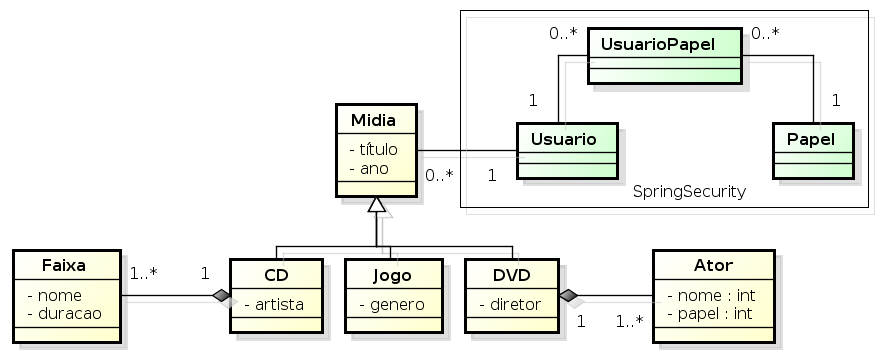
\includegraphics[width=14cm]{Midia}
\caption{Catálogo de Mídias.}
\label{MidiaFig}
\end{figure}

\subsection*{\underline{Entidade {\bf Midia}}}

A entidade  {\bf Midia} é uma  classe abstrata que deverá  conter atributos para
armazenar  os seguintes  dados  sobre as  mídias:  {\bf título}  e  {\bf ano  de
  criação}.

\subsection*{\underline{Entidade {\bf CD}}}

A entidade {\bf CD} (subclasse de {\bf Midia}) é uma classe que representa um CD
de  música e  deve  conter atributos  para  armazenar os  seguintes dados:  {\bf
  artista} (compositor/interpréte da  obra) e {\bf a lista  de faixas} (entidade
{\bf Faixa}). Vale a pena salientar que é um relacionamento {\bf 1 para N} entre
{\bf CD} e {\bf Faixa}.

\subsection*{\underline{Entidade {\bf Faixa}}}

A entidade {\bf  Faixa} é uma classe  que representa uma faixa de  música e deve
conter os seguintes  atributos: {\bf nome} da faixa e {\bf  duração} da faixa em
segundos.

\subsection*{\underline{Classe {\bf Jogo}}}

A classe {\bf  Jogo} (subclasse de {\bf Midia}) representa  um jogo eletrônico e
deve  conter o  seguinte atributo:  {\bf gênero}  do jogo  eletrônico (Esportes,
Corrida, RPG, Aventura, Tabuleiro, etc).

\subsection*{\underline{Entidade {\bf DVD}}}

A entidade {\bf  DVD} (subclasse de {\bf Midia}) é uma  classe que representa um
filme em  DVD e deve  conter atributos para  armazenar os seguintes  dados: {\bf
  diretor} do filme  e uma {\bf lista dos  principais atores/artistas} (entidade
{\bf Ator}) que atuaram no filme e  o papel desempenhado no filme.  Vale a pena
salientar que é um relacionamento {\bf 1 para N} entre {\bf DVD} e {\bf Ator}.

\subsection*{\underline{Entidade {\bf Ator}}}

A entidade  {\bf Ator} é uma classe  que representa um ator/atriz  e deve conter
atributos para armazenar os seguintes dados: o {\bf nome} do ator/atriz e o {\bf
  papel} desempenhado no filme .  

\subsection*{\underline{Entidades {\bf Usuario}, {\bf Papel} e {\bf UsuarioPapel}}}

A entidade {\bf Usuario} é uma classe que representa os usuário do sistema. Cada
usuário terá uma coleção de mídias (entidade {\bf Midia}) associadas a ele. Vale
a pena salientar  que é um relacionamento  {\bf 1 para N} entre  {\bf Usuario} e
{\bf Midia}  (As mídias  são categorizados em:  CDs de  música, filmes em  DVD e
jogos). 

\hspace{1cm}\\
\noindent A  entidade {\bf Papel} é uma  classe que representa os  papéis que os
usuários podem desempenhar.  Cada papel possui  permissões a ele associadas.  

\hspace{1cm}\\
\noindent  A  entidade  {\bf  UsuarioPapel}   é  uma  classe  que  representa  o
relacionamento muitos-para-muitos  entre usuários e papéis. Ou  seja, um usuário
pode  desempenhar vários  papeis e  um papel  pode ser  desempenhado  por vários
usuários.  

\hspace{1cm}\\
\noindent As entidades {\bf Usuario}, {\bf Papel} e {\bf UsuarioPapel} devem ser
geradas  através do  comando  {\bf  s2-quickstart} discutido  no  capítulo 3  do
material.  

\newpage

\section*{Observações importantes}

\vspace{0.3cm}

\begin{itemize}

\item É necessário a utilização do {\bf mecanismo de herança} e associações {\bf
  1 para N} para a implementação do catálogo.

\vspace{0.2cm}

\item Internacionalização (I18n)

\vspace{0.2cm}

\begin{itemize}

\item Português e uma língua estrangeira (Inglês, Francês, Alemão, Japonês, etc)

\end{itemize}

\vspace{0.2cm}

\item Autenticação

\vspace{0.2cm}

\begin{itemize}

\item  Simples: login/senha  (armazenado em  banco  de dados)  da entidade  {\bf
  Usuario}.  

\end{itemize}

\vspace{0.2cm}

\item Versão {\it grails} (mínimo): 3.1.4

\end{itemize}

% \section*{Funcionalidade: apresentar detalhes}

% \vspace{0.3cm}

% É  necessária a implementação  da funcionalidade  {\bf apresentar  detalhes} das mídias levando em consideração o tipo da mídia. Essa funcionalidade precisa está associada a  funcionalidade de  listagem das mídias.  Ou seja, quando  o usuário selecionar uma mídia, os seus detalhes precisam ser apresentados. 

% \begin{enumerate}

% \vspace{0.2cm}

% \item Detalhes de um CD de música

% \hspace{1cm}\\
% \begin{tabular}{|l|}
% \hline Título: Bachianas Brasileiras No.2 \\

% Ano: 2004 \\

% Tipo: CD de música \\

% Artista: Orquestra de Câmara da Universidade de São Paulo \\

% Faixa 1: (Prelúdio) O Canto do Capadócio, duracão: 8:32 \\

% Faixa 2: (Ária) O Canto da Nossa Terra, duracao: 6:29 \\

% Faixa 3: (Dança) Lembranca do Sertão, duracão: 5:24 \\

% Faixa 4: (Tocata) O Trenzinho do Caipira, duracão: 4:44 \\

% \hline
% \end{tabular}
% \newline

% \vspace{0.2cm}
% \item Detalhes de um filme em DVD

% \hspace{1cm}\\
% \begin{tabular}{|l|}
% \hline Título: O Senhor dos Anéis - A Sociedade dos Anéis \\

% Ano: 2001 \\

% Tipo: Filme em DVD \\

% Diretor: Peter Jackson \\

% Artista 1: Elijah Wood, papel: Frodo Baggins \\

% Artista 2: Viggo Mortensen, papel: Aragorn \\

% Artista 3: Orlando Bloom, papel: Legolas Greenleaf \\

% Artista 4: Christopher Lee, papel: Saruman \\

% Artista 5: Ian McKellen, papel: Gandalf \\

% \hline
% \end{tabular}
% \newline

% \vspace{0.2cm}
% \item Detalhes de um jogo

% \hspace{1cm}\\
% \begin{tabular}{|l|}
% \hline Título: {\it Need For Speed - Underground II} \\

% Ano: 2005 \\

% Tipo: Jogo Eletrônico \\

% Gênero: Corrida \\ \hline
% \end{tabular}

% \end{enumerate}

% \newpage

\section*{Funcionalidade: redirecionamento}

\vspace{0.3cm}

Implemente  uma página  de {\it  login} que  autentica os  usuários e  realiza o
direcionamento dependente do papel do usuário: 

\vspace{0.3cm}

\begin{itemize}

\item  Se papel  do usuário  é  {\bf Administrador},  direcione para  a lista  de
  usuários.

\vspace{0.3cm}

\item Se papel do usuário é {\bf Comum}, direcione para a lista de CDs do usuário
  logado.

\end{itemize}

% \section*{Funcionalidade: lista de CDs (apenas para RAs pares)}

% \vspace{0.3cm}

% \begin{itemize}

% \item Implemente a funcionalidade (página {\it  web}) de busca de CDs: com ajuda no preenchimento (autocomplete em AJAX) do nome do CD.  
 
% \vspace{0.3cm}

% \item Implemente um serviço web que retorna a lista de CDs de um dado artista: o parâmetro de entrada do serviço web é o nome do artista.

% \end{itemize}

% \section*{Funcionalidade: lista de DVDs (apenas para RAs ímpares)}

% \vspace{0.3cm}

% \begin{itemize}

% \item Implemente a funcionalidade (página {\it web}) de busca de DVDs: com ajuda no preenchimento (autocomplete em AJAX) do nome do DVD.  
 
% \vspace{0.3cm}

% \item Implemente um serviço web que retorna  a lista de DVDs de um dado diretor: o parâmetro de entrada do serviço web é o nome do diretor.

% \end{itemize}

% \vspace{0.3cm}








%-------------------------------------------------------------------------------
%	BIBLIOGRAPHY
%-------------------------------------------------------------------------------

%\chapter*{Bibliography}
\bibliographystyle{plain}
\bibliography{bib/EngWeb}

%-------------------------------------------------------------------------------
%	INDEX
%-------------------------------------------------------------------------------

\cleardoublepage
\setlength{\columnsep}{0.75cm}
\addcontentsline{toc}{chapter}{\textcolor{ocre}{Índice Remissivo}}
\printindex

%-------------------------------------------------------------------------------

\end{document}
